\expandafter\ifx\csname MasterFile\endcsname\relax
	\def\SubFile{hoge}
	\documentclass[a4j,12pt,twoside,openany]{jreport}
%\nofiles %tocファイルを更新させない
%\documentclass[12pt,a4j,twoside,openany]{jsbook}
\usepackage[dvipdfmx]{graphicx}
\usepackage{../dspc} % ベースラインスキップの指定
\usepackage{../slashbox} % 表に斜線を入れる
%\usepackage{../mediabb}
\usepackage{fancyvrb} % Verbatim環境
\usepackage{fancyhdr} % Headerの下線付き章見出し
\usepackage{here} % float[H]
\usepackage{multirow}
\usepackage{hhline} % 表の罫線の角を美しくする
\usepackage{amsmath} %コレがないとcasesが動かない
\usepackage{amsfonts} % 数学用フォント
\usepackage{bm} % 数式環境での bold
\usepackage{algorithm}
\usepackage{algorithmicx}
\usepackage[noend]{algpseudocode}%\procedureはここに含まれる
\usepackage[flushleft]{threeparttable} % 脚注付きテーブル
\usepackage{enumitem}
\usepackage{comment}
\usepackage{fancybox}
%\usepackage{csvsimple,booktabs,siunitx}
%\usepackage{filecontents}
\usepackage{ulinej}


\setlength{\evensidemargin}{5pt}
\setlength{\oddsidemargin}{40pt}
%\setlength{\headheight}{16.5pt}
%%\setlength{\headheight}{30pt}
\setcounter{secnumdepth}{3}
\setlist[description]{leftmargin=2\parindent,labelindent=\parindent}

\makeatletter
\def\@makechapterhead#1{%
	\vspace*{50\p@}%
	{
		\parindent \z@ \raggedright \normalfont
		\ifnum \c@secnumdepth >\m@ne
		% \if@mainmatter
			\huge\bfseries\@chapapp\thechapter\@chappos
			\par\nobreak
			\vskip 20\p@
		% \fi
		\fi
		\interlinepenalty\@M
		\Huge\bfseries #1\par\nobreak
		\vskip 40\p@
	}
}

%新しいコマンド定義
\newcounter{linenumber}
\newenvironment{listing}{%
  \begin{list}{%
    \small\arabic{linenumber}:}{%
      \usecounter{linenumber}%
      \setlength{\baselineskip}{18pt}%
      \setlength{\itemsep}{0pt}%
      \setlength{\parsep}{0pt}}}%
 {\end{list}}
\newcommand{\figcaption}[1]{\def\@captype{figure}\caption{#1}}
\newcommand{\tblcaption}[1]{\def\@captype{table}\caption{#1}}
\newcommand{\norm}[1]{\left\| #1 \right\|}
\newcommand{\cc}[1]{\multicolumn{1}{|c|}{#1}}
\newcommand{\circled}[1]{\raisebox{.5pt}{\textcircled{\raisebox{-.9pt} {#1}}}}
\newcommand{\specialcell}[2][c]{%
  \begin{tabular}[#1]{@{}c@{}}#2\end{tabular}}
\makeatother
%===============================================================================
\expandafter\ifx\csname SubFile\endcsname\relax
\begin{document}
\def\MasterFile{hoge}
%-------------------------------------------------------------------------------
%\maketitle
\thispagestyle{empty}
\documentclass[a4j,12pt]{jarticle}
% 外表紙

% 題名
\def\title{降水量予測のための\\Sequence-to-Sequenceモデルに基づく\\マルチモーダル学習}
% 著者
\def\author{林 政行}
% 入学年度(平成)
\def\year{24}
% 学籍番号
\def\number{24115113}
% 指導教官
\def\kyoukan{伊藤孝行}
% 指導教官役職
\def\kyoukanrank{教授}
% 提出日
\def\teisyutubi{平成28年2月8日}

\begin{document}
\pagestyle{empty}
\baselineskip=18pt

\begin{center}

\vspace*{2cm}

{\huge \textbf{卒業論文}}

\vspace*{3cm}

%\vrule width 10cm height 1pt depth 0pt



%(題目)
%\vspace{5pt}
%\hrule height 3pt
%\vspace{1zh}

\vrule width 6.25cm height 6pt depth -2pt
\makebox[1.5cm]{(題目)}
\vrule width 6.25cm height 6pt depth -2pt

{\LARGE {\title}}

\vspace{1zh}
%{\large {\subtitle}}
%\hrule height 3pt
\vrule width 14cm height 4pt depth 0pt

\vspace*{1cm}

指導教員 {\large {\kyoukan}} {\kyoukanrank}

%\vspace*{5cm}
\vfill

{\large 名古屋工業大学 情報工学科}

{\large 平成{\year}年度 入学 ({\number})}

\vspace*{1cm}

%{\huge\mc {\author}}

\underline{(氏名)\hspace{3zw}{\huge\mc {\author}}\hspace{3zw}}

\vspace*{1cm}

({\teisyutubi}提出)

\vspace{2cm}
\end{center}

\end{document}
\begin{titlepage}

% 題名
\def\title{分散表現を用いた\\話題変化判定}
% 補助題名
\def\subtitle{卒業論文}
% 著者
\def\author{芳野 魁}
% 入学年度(平成)
\def\year{29}
% 学籍番号
\def\number{26115162}
% 指導教官
\def\kyoukan{伊藤 孝行}
% 指導教官役職
\def\kyoukanrank{教授}
% 提出日
\def\teisyutubi{平成29年9月19日}

\pagestyle{empty}

\begin{center}

\vspace*{20mm}
{\Large\mc 平成29年度 \hspace{7mm} 卒 業 論 文}
\vspace{15mm}

%\setlength{\unitlength}{1mm}
\begin{picture}(100,60)
  \put(0,0){\makebox(100,60){\huge\bf\shortstack{\title}}}
\end{picture}
\\
%\begin{picture}(100,5)
%  \put(0,0){\makebox(100,5){\Large\bf\shortstack{\subtitle}}}
%\end{picture}
\end{center}
\vspace{10mm}
\begin{flushright}
\begin{tabular}{ll}
{\large 提出日} & {\large {\teisyutubi}} \\
{\large 所属}  & {\large 名古屋工業大学 情報工学科} \\
{\large 指導教員} & {\large {\kyoukan} {\kyoukanrank}} \\
 & \\
{\large 入学年度} & {\large 平成{\year}年度入学}\\
{\large 学籍番号} &{\large {\number}} \\
 & \\
%{\large 氏名} & {\huge {\author}}
{\large 氏名} & {\huge\mc {\author}}
\end{tabular}
\end{flushright}

\end{titlepage}

%\addcontentsline{toc}{chapter}{表紙}
\thispagestyle{empty}
\mbox{}\newpage
%===============================================================================
%\frontmatter
%===============================================================================
%\mainmatter
%-------------------------------------------------------------------------------
\pagenumbering{arabic}
\cleardoublepage
\expandafter\ifx\csname MasterFile\endcsname\relax
\def\SubFile{hoge}
\documentclass[a4j,12pt,twoside,openany]{jreport}
%\nofiles %tocファイルを更新させない
%\documentclass[12pt,a4j,twoside,openany]{jsbook}
\usepackage[dvipdfmx]{graphicx}
\usepackage{../dspc} % ベースラインスキップの指定
\usepackage{../slashbox} % 表に斜線を入れる
%\usepackage{../mediabb}
\usepackage{fancyvrb} % Verbatim環境
\usepackage{fancyhdr} % Headerの下線付き章見出し
\usepackage{here} % float[H]
\usepackage{multirow}
\usepackage{hhline} % 表の罫線の角を美しくする
\usepackage{amsmath} %コレがないとcasesが動かない
\usepackage{amsfonts} % 数学用フォント
\usepackage{bm} % 数式環境での bold
\usepackage{algorithm}
\usepackage{algorithmicx}
\usepackage[noend]{algpseudocode}%\procedureはここに含まれる
\usepackage[flushleft]{threeparttable} % 脚注付きテーブル
\usepackage{enumitem}
\usepackage{comment}
\usepackage{fancybox}
%\usepackage{csvsimple,booktabs,siunitx}
%\usepackage{filecontents}
\usepackage{ulinej}


\setlength{\evensidemargin}{5pt}
\setlength{\oddsidemargin}{40pt}
%\setlength{\headheight}{16.5pt}
%%\setlength{\headheight}{30pt}
\setcounter{secnumdepth}{3}
\setlist[description]{leftmargin=2\parindent,labelindent=\parindent}

\makeatletter
\def\@makechapterhead#1{%
	\vspace*{50\p@}%
	{
		\parindent \z@ \raggedright \normalfont
		\ifnum \c@secnumdepth >\m@ne
		% \if@mainmatter
			\huge\bfseries\@chapapp\thechapter\@chappos
			\par\nobreak
			\vskip 20\p@
		% \fi
		\fi
		\interlinepenalty\@M
		\Huge\bfseries #1\par\nobreak
		\vskip 40\p@
	}
}

%新しいコマンド定義
\newcounter{linenumber}
\newenvironment{listing}{%
  \begin{list}{%
    \small\arabic{linenumber}:}{%
      \usecounter{linenumber}%
      \setlength{\baselineskip}{18pt}%
      \setlength{\itemsep}{0pt}%
      \setlength{\parsep}{0pt}}}%
 {\end{list}}
\newcommand{\figcaption}[1]{\def\@captype{figure}\caption{#1}}
\newcommand{\tblcaption}[1]{\def\@captype{table}\caption{#1}}
\newcommand{\norm}[1]{\left\| #1 \right\|}
\newcommand{\cc}[1]{\multicolumn{1}{|c|}{#1}}
\newcommand{\circled}[1]{\raisebox{.5pt}{\textcircled{\raisebox{-.9pt} {#1}}}}
\newcommand{\specialcell}[2][c]{%
  \begin{tabular}[#1]{@{}c@{}}#2\end{tabular}}
\makeatother
%===============================================================================
\expandafter\ifx\csname SubFile\endcsname\relax
\begin{document}
\def\MasterFile{hoge}
%-------------------------------------------------------------------------------
%\maketitle
\thispagestyle{empty}
\input{../hyoushi/hyoushi}
\input{../hyoushi/title}
%\addcontentsline{toc}{chapter}{表紙}
\thispagestyle{empty}
\mbox{}\newpage
%===============================================================================
%\frontmatter
%===============================================================================
%\mainmatter
%-------------------------------------------------------------------------------
\pagenumbering{arabic}
\cleardoublepage
\input{../0.Abstract/chapter}
%-------------------------------------------------------------------------------
\clearpage
\addcontentsline{toc}{chapter}{目次}
\tableofcontents

\clearpage
\addcontentsline{toc}{chapter}{図目次}
\listoffigures

\clearpage
\addcontentsline{toc}{chapter}{表目次}
\listoftables

%-------------------------------------------------------------------------------

%=====================
\pagestyle{fancy} % Headerをつける
\renewcommand{\sectionmark}[1]{\markright{\thesection\ \ \ #1}}
\renewcommand{\chaptermark}[1]{\markboth{#1}{}}
\lhead{}
\chead{}
\lfoot{}
\rfoot{}%-------------------------------------------------------------------------------
\input{../1.Introduction/chapter}
%-------------------------------------------------------------------------------
\input{../2.Related_Work/chapter}
%-------------------------------------------------------------------------------
\input{../3.The_Model/chapter}
%-------------------------------------------------------------------------------
\input{../4.Implementation/chapter}
%-------------------------------------------------------------------------------
\input{../5.Experiments/chapter}
%-------------------------------------------------------------------------------
\input{../6.Conclusion/chapter}

%===============================================================================
\pagestyle{plain}
%-------------------------------------------------------------------------------
\input{../7.Acknowledgement/chapter} %謝辞
%-------------------------------------------------------------------------------
\def\BibFile{../Bibliograhoy/database2}
\input{../Bibliography/chapter} %参考文献
% %===============================================================================
\appendix
\input{../A.Mypaper/chapter} % 投稿論文リスト
\input{../B.SIG-CCI2/chapter} %
\input{../C.IPSJ80/chapter} %
\input{../D.TopicGraph/chapter} %
%===============================================================================
\end{document}\input{../../../../../../../Downloads/2章.docx}

\fi

\begin{document}
\fi
%-------------------------------------------------------------------------------
\cleardoublepage
\chapter*{論文要旨}\addcontentsline{toc}{chapter}{論文要旨}
近年,Web上での大規模な議論活動が活発になっているが,現在一般的に使われている "2ちゃんねる" や "Twitter" といったシステムでは整理や収束を行うことが困難である.困難である原因として,議論の管理を行う者がいないことが挙げられる.
議論を収束させるには議論のマネジメントを行う人物が必要である.
%
大規模意見集約システムCOLLAGREEではファシリテーターと呼ばれる人物が議論のマネジメントを行っている.
しかし,ファシリテーターは人間であり,長時間に渡って大人数での議論の動向をマネジメントし続けるのは困難である.
%
COLLAGREEで大規模な議論を収束させるためには,ファシリテーターが必要な時にだけ画面を見るようにして画面に向き合う時間を減らす工夫があることが望ましい.ファシリテーターが画面を見るべきタイミングは議論の話題が変化したときである.以前の議論の内容から外れた発言がされた時,ファシリテーターが適切に発言することで,脱線や炎上を避けて議論を収束させることができる.
すなわち,ファシリテーターの代わりに自動的に議論中の話題の変化を事前に判定することが求められている.
%
現在,COLLAGREE上で使用されている議論支援システムは投稿支援システムと議論可視化システムの2つに大別できる.
投稿支援システムはポイント機能やファシリテーションフレーズ簡易投稿機能のように,ユーザーが投稿をする際に何らかの補助やリアクションを行う.現行の機能では選択肢の提示に留まっており,作業量を減らすことには繋がりにくい。
一方,議論可視化システムは議論ツリーやキーワード抽出のように,ユーザーにスレッドとは異なる議論の見方を提供する.現行の機能では議論を見やすくすることに重点が置かれており,議論の把握の助けにはなるが画面に向き合う時間を減らすことにはなりにくい.むしろ,作業量を増やすことになり得る機能もある.
\begin{comment}
ポイント機能(ユーザの議論行動を活性化)-1
ファシリテーションフレーズ簡易投稿機能-1
議論ツリー-2
1文の要約,スレッドの要約,クラスタリング,返信意見の極性判定-2
ファシリテーションスタンプ-1
キーワード抽出-2
いいね機能-1
いいねランキング-2
投票機能-1
議論フェーズ機能-2
1-意見を出す、投稿をする際に補助や選択肢、リアクションを与える
2-議論の別の見方を提供する
\end{comment}
%
近年,自然言語処理の分野において分散表現が多くの研究で使われており,機械翻訳を始めとする単語の意味が重要となる分野で精度の向上が確認されている.分散表現を用いることで,人間に近い精度で話題の変化を観測することが可能となる.
%
以上のような背景を踏まえて,分散表現を用いて,話題の変化を観測し,話題の変化が確認された時にファシリテーターに伝えることが望ましい.
話題の変化の観測は,発言中に現れる単語の関連度合いの計算と見なすことができる.
分散表現を用いることで単語間の類似度を求めることができる,値が大きいほど単語がそれぞれ類似した実数ベクトルであることを表す.単語Aと単語Bの実数ベクトルが類似しているとは,単語Aと共に使われることの多い単語と単語Bと共に使われることの多い単語が多く共通していることを示す.故に,分散表現を使って単語の関連度を計算することができる.
%
発言文から単語を選ぶ際には自動要約を用いる.発言文から重要でない単語を取り除くことで関連度の計算の精度を高めることが可能となる.
%
本論文では,分散表現を用いて議論中での発言に含まれる単語の関連度を計算し,話題の変化を観測する手法を提案する.
%
提案手法は,既存の抽出的要約手法を用いて選ばれた単語の関連度を計算する手法,Seq2Seqによる生成的要約を用いて生成された単語の関連度を計算する手法,オントロジーを用いて求められた単語の関連度を計算する手法の3つである.
提案した3つの手法により,議論中の話題の変化の観測の評価実験を行い,各手法の評価を行う.
評価実験によって,提案手法を用いることで人間の代わりに自動的に話題の変化を観測できることを確認する.
%
 \begin{comment}
大規模な議論では意見を共有することは可能であるが,議論を整理させることや収束させることは難しい.以上から大規模意見集約システムCOLLAGREEが開発された.本システムではWeb上で適切に大規模な議論を行うことができるように議論をマネジメントするファシリテーターを導入した.
過去の実験ではファシリテーターの存在が議論の集約に大きな役割を果たしていることが認識されており,大規模な議論のためにファシリテータは必要である.しかし,議論の規模に伴って議論時間が長くなる傾向があり,同時にファシリテーターは常に議論の動向を見続ける必要がある.故に,議論の規模が大きくなればなるほどファシリテーターは長時間かつ大規模な議論の動向の監視によって大きな負担がかかる.大規模な議論が増加する傾向を踏まえるとファシリテーターにかかる負担を軽減する支援が必要となることは明白である.
また,近年自然言語処理の分野において分散表現が多くの研究で使われており,機械翻訳を始めとする複数の分野で精度の向上が確認されている.まだ適応されていない分野でも結果の向上が期待できる.
従って,本研究では負担軽減の1つとして分散表現を用いて議論中での話題の変化を人間の代わりに検知することでファシリテーターの負担を軽減することを目指す.
-----------------

\end{comment}
%-------------------------------------------------------------------------------
\expandafter\ifx\csname MasterFile\endcsname\relax
\end{document}
\fi

%-------------------------------------------------------------------------------
\clearpage
\addcontentsline{toc}{chapter}{目次}
\tableofcontents

\clearpage
\addcontentsline{toc}{chapter}{図目次}
\listoffigures

\clearpage
\addcontentsline{toc}{chapter}{表目次}
\listoftables

%-------------------------------------------------------------------------------

%=====================
\pagestyle{fancy} % Headerをつける
\renewcommand{\sectionmark}[1]{\markright{\thesection\ \ \ #1}}
\renewcommand{\chaptermark}[1]{\markboth{#1}{}}
\lhead{}
\chead{}
\lfoot{}
\rfoot{}%-------------------------------------------------------------------------------
\expandafter\ifx\csname MasterFile\endcsname\relax
\def\SubFile{hoge}
\documentclass[a4j,12pt,twoside,openany]{jreport}
%\nofiles %tocファイルを更新させない
%\documentclass[12pt,a4j,twoside,openany]{jsbook}
\usepackage[dvipdfmx]{graphicx}
\usepackage{../dspc} % ベースラインスキップの指定
\usepackage{../slashbox} % 表に斜線を入れる
%\usepackage{../mediabb}
\usepackage{fancyvrb} % Verbatim環境
\usepackage{fancyhdr} % Headerの下線付き章見出し
\usepackage{here} % float[H]
\usepackage{multirow}
\usepackage{hhline} % 表の罫線の角を美しくする
\usepackage{amsmath} %コレがないとcasesが動かない
\usepackage{amsfonts} % 数学用フォント
\usepackage{bm} % 数式環境での bold
\usepackage{algorithm}
\usepackage{algorithmicx}
\usepackage[noend]{algpseudocode}%\procedureはここに含まれる
\usepackage[flushleft]{threeparttable} % 脚注付きテーブル
\usepackage{enumitem}
\usepackage{comment}
\usepackage{fancybox}
%\usepackage{csvsimple,booktabs,siunitx}
%\usepackage{filecontents}
\usepackage{ulinej}


\setlength{\evensidemargin}{5pt}
\setlength{\oddsidemargin}{40pt}
%\setlength{\headheight}{16.5pt}
%%\setlength{\headheight}{30pt}
\setcounter{secnumdepth}{3}
\setlist[description]{leftmargin=2\parindent,labelindent=\parindent}

\makeatletter
\def\@makechapterhead#1{%
	\vspace*{50\p@}%
	{
		\parindent \z@ \raggedright \normalfont
		\ifnum \c@secnumdepth >\m@ne
		% \if@mainmatter
			\huge\bfseries\@chapapp\thechapter\@chappos
			\par\nobreak
			\vskip 20\p@
		% \fi
		\fi
		\interlinepenalty\@M
		\Huge\bfseries #1\par\nobreak
		\vskip 40\p@
	}
}

%新しいコマンド定義
\newcounter{linenumber}
\newenvironment{listing}{%
  \begin{list}{%
    \small\arabic{linenumber}:}{%
      \usecounter{linenumber}%
      \setlength{\baselineskip}{18pt}%
      \setlength{\itemsep}{0pt}%
      \setlength{\parsep}{0pt}}}%
 {\end{list}}
\newcommand{\figcaption}[1]{\def\@captype{figure}\caption{#1}}
\newcommand{\tblcaption}[1]{\def\@captype{table}\caption{#1}}
\newcommand{\norm}[1]{\left\| #1 \right\|}
\newcommand{\cc}[1]{\multicolumn{1}{|c|}{#1}}
\newcommand{\circled}[1]{\raisebox{.5pt}{\textcircled{\raisebox{-.9pt} {#1}}}}
\newcommand{\specialcell}[2][c]{%
  \begin{tabular}[#1]{@{}c@{}}#2\end{tabular}}
\makeatother
%===============================================================================
\expandafter\ifx\csname SubFile\endcsname\relax
\begin{document}
\def\MasterFile{hoge}
%-------------------------------------------------------------------------------
%\maketitle
\thispagestyle{empty}
\input{../hyoushi/hyoushi}
\input{../hyoushi/title}
%\addcontentsline{toc}{chapter}{表紙}
\thispagestyle{empty}
\mbox{}\newpage
%===============================================================================
%\frontmatter
%===============================================================================
%\mainmatter
%-------------------------------------------------------------------------------
\pagenumbering{arabic}
\cleardoublepage
\input{../0.Abstract/chapter}
%-------------------------------------------------------------------------------
\clearpage
\addcontentsline{toc}{chapter}{目次}
\tableofcontents

\clearpage
\addcontentsline{toc}{chapter}{図目次}
\listoffigures

\clearpage
\addcontentsline{toc}{chapter}{表目次}
\listoftables

%-------------------------------------------------------------------------------

%=====================
\pagestyle{fancy} % Headerをつける
\renewcommand{\sectionmark}[1]{\markright{\thesection\ \ \ #1}}
\renewcommand{\chaptermark}[1]{\markboth{#1}{}}
\lhead{}
\chead{}
\lfoot{}
\rfoot{}%-------------------------------------------------------------------------------
\input{../1.Introduction/chapter}
%-------------------------------------------------------------------------------
\input{../2.Related_Work/chapter}
%-------------------------------------------------------------------------------
\input{../3.The_Model/chapter}
%-------------------------------------------------------------------------------
\input{../4.Implementation/chapter}
%-------------------------------------------------------------------------------
\input{../5.Experiments/chapter}
%-------------------------------------------------------------------------------
\input{../6.Conclusion/chapter}

%===============================================================================
\pagestyle{plain}
%-------------------------------------------------------------------------------
\input{../7.Acknowledgement/chapter} %謝辞
%-------------------------------------------------------------------------------
\def\BibFile{../Bibliograhoy/database2}
\input{../Bibliography/chapter} %参考文献
% %===============================================================================
\appendix
\input{../A.Mypaper/chapter} % 投稿論文リスト
\input{../B.SIG-CCI2/chapter} %
\input{../C.IPSJ80/chapter} %
\input{../D.TopicGraph/chapter} %
%===============================================================================
\end{document}\input{../../../../../../../Downloads/2章.docx}

\fi

\begin{document}
\fi
%-------------------------------------------------------------------------------
\cleardoublepage
\chapter*{論文要旨}\addcontentsline{toc}{chapter}{論文要旨}
近年,Web上での大規模な議論活動が活発になっているが,現在一般的に使われている "2ちゃんねる" や "Twitter" といったシステムでは整理や収束を行うことが困難である.困難である原因として,議論の管理を行う者がいないことが挙げられる.
議論を収束させるには議論のマネジメントを行う人物が必要である.
%
大規模意見集約システムCOLLAGREEではファシリテーターと呼ばれる人物が議論のマネジメントを行っている.
しかし,ファシリテーターは人間であり,長時間に渡って大人数での議論の動向をマネジメントし続けるのは困難である.
%
COLLAGREEで大規模な議論を収束させるためには,ファシリテーターが必要な時にだけ画面を見るようにして画面に向き合う時間を減らす工夫があることが望ましい.ファシリテーターが画面を見るべきタイミングは議論の話題が変化したときである.以前の議論の内容から外れた発言がされた時,ファシリテーターが適切に発言することで,脱線や炎上を避けて議論を収束させることができる.
すなわち,ファシリテーターの代わりに自動的に議論中の話題の変化を事前に判定することが求められている.
%
現在,COLLAGREE上で使用されている議論支援システムは投稿支援システムと議論可視化システムの2つに大別できる.
投稿支援システムはポイント機能やファシリテーションフレーズ簡易投稿機能のように,ユーザーが投稿をする際に何らかの補助やリアクションを行う.現行の機能では選択肢の提示に留まっており,作業量を減らすことには繋がりにくい。
一方,議論可視化システムは議論ツリーやキーワード抽出のように,ユーザーにスレッドとは異なる議論の見方を提供する.現行の機能では議論を見やすくすることに重点が置かれており,議論の把握の助けにはなるが画面に向き合う時間を減らすことにはなりにくい.むしろ,作業量を増やすことになり得る機能もある.
\begin{comment}
ポイント機能(ユーザの議論行動を活性化)-1
ファシリテーションフレーズ簡易投稿機能-1
議論ツリー-2
1文の要約,スレッドの要約,クラスタリング,返信意見の極性判定-2
ファシリテーションスタンプ-1
キーワード抽出-2
いいね機能-1
いいねランキング-2
投票機能-1
議論フェーズ機能-2
1-意見を出す、投稿をする際に補助や選択肢、リアクションを与える
2-議論の別の見方を提供する
\end{comment}
%
近年,自然言語処理の分野において分散表現が多くの研究で使われており,機械翻訳を始めとする単語の意味が重要となる分野で精度の向上が確認されている.分散表現を用いることで,人間に近い精度で話題の変化を観測することが可能となる.
%
以上のような背景を踏まえて,分散表現を用いて,話題の変化を観測し,話題の変化が確認された時にファシリテーターに伝えることが望ましい.
話題の変化の観測は,発言中に現れる単語の関連度合いの計算と見なすことができる.
分散表現を用いることで単語間の類似度を求めることができる,値が大きいほど単語がそれぞれ類似した実数ベクトルであることを表す.単語Aと単語Bの実数ベクトルが類似しているとは,単語Aと共に使われることの多い単語と単語Bと共に使われることの多い単語が多く共通していることを示す.故に,分散表現を使って単語の関連度を計算することができる.
%
発言文から単語を選ぶ際には自動要約を用いる.発言文から重要でない単語を取り除くことで関連度の計算の精度を高めることが可能となる.
%
本論文では,分散表現を用いて議論中での発言に含まれる単語の関連度を計算し,話題の変化を観測する手法を提案する.
%
提案手法は,既存の抽出的要約手法を用いて選ばれた単語の関連度を計算する手法,Seq2Seqによる生成的要約を用いて生成された単語の関連度を計算する手法,オントロジーを用いて求められた単語の関連度を計算する手法の3つである.
提案した3つの手法により,議論中の話題の変化の観測の評価実験を行い,各手法の評価を行う.
評価実験によって,提案手法を用いることで人間の代わりに自動的に話題の変化を観測できることを確認する.
%
 \begin{comment}
大規模な議論では意見を共有することは可能であるが,議論を整理させることや収束させることは難しい.以上から大規模意見集約システムCOLLAGREEが開発された.本システムではWeb上で適切に大規模な議論を行うことができるように議論をマネジメントするファシリテーターを導入した.
過去の実験ではファシリテーターの存在が議論の集約に大きな役割を果たしていることが認識されており,大規模な議論のためにファシリテータは必要である.しかし,議論の規模に伴って議論時間が長くなる傾向があり,同時にファシリテーターは常に議論の動向を見続ける必要がある.故に,議論の規模が大きくなればなるほどファシリテーターは長時間かつ大規模な議論の動向の監視によって大きな負担がかかる.大規模な議論が増加する傾向を踏まえるとファシリテーターにかかる負担を軽減する支援が必要となることは明白である.
また,近年自然言語処理の分野において分散表現が多くの研究で使われており,機械翻訳を始めとする複数の分野で精度の向上が確認されている.まだ適応されていない分野でも結果の向上が期待できる.
従って,本研究では負担軽減の1つとして分散表現を用いて議論中での話題の変化を人間の代わりに検知することでファシリテーターの負担を軽減することを目指す.
-----------------

\end{comment}
%-------------------------------------------------------------------------------
\expandafter\ifx\csname MasterFile\endcsname\relax
\end{document}
\fi

%-------------------------------------------------------------------------------
\expandafter\ifx\csname MasterFile\endcsname\relax
\def\SubFile{hoge}
\documentclass[a4j,12pt,twoside,openany]{jreport}
%\nofiles %tocファイルを更新させない
%\documentclass[12pt,a4j,twoside,openany]{jsbook}
\usepackage[dvipdfmx]{graphicx}
\usepackage{../dspc} % ベースラインスキップの指定
\usepackage{../slashbox} % 表に斜線を入れる
%\usepackage{../mediabb}
\usepackage{fancyvrb} % Verbatim環境
\usepackage{fancyhdr} % Headerの下線付き章見出し
\usepackage{here} % float[H]
\usepackage{multirow}
\usepackage{hhline} % 表の罫線の角を美しくする
\usepackage{amsmath} %コレがないとcasesが動かない
\usepackage{amsfonts} % 数学用フォント
\usepackage{bm} % 数式環境での bold
\usepackage{algorithm}
\usepackage{algorithmicx}
\usepackage[noend]{algpseudocode}%\procedureはここに含まれる
\usepackage[flushleft]{threeparttable} % 脚注付きテーブル
\usepackage{enumitem}
\usepackage{comment}
\usepackage{fancybox}
%\usepackage{csvsimple,booktabs,siunitx}
%\usepackage{filecontents}
\usepackage{ulinej}


\setlength{\evensidemargin}{5pt}
\setlength{\oddsidemargin}{40pt}
%\setlength{\headheight}{16.5pt}
%%\setlength{\headheight}{30pt}
\setcounter{secnumdepth}{3}
\setlist[description]{leftmargin=2\parindent,labelindent=\parindent}

\makeatletter
\def\@makechapterhead#1{%
	\vspace*{50\p@}%
	{
		\parindent \z@ \raggedright \normalfont
		\ifnum \c@secnumdepth >\m@ne
		% \if@mainmatter
			\huge\bfseries\@chapapp\thechapter\@chappos
			\par\nobreak
			\vskip 20\p@
		% \fi
		\fi
		\interlinepenalty\@M
		\Huge\bfseries #1\par\nobreak
		\vskip 40\p@
	}
}

%新しいコマンド定義
\newcounter{linenumber}
\newenvironment{listing}{%
  \begin{list}{%
    \small\arabic{linenumber}:}{%
      \usecounter{linenumber}%
      \setlength{\baselineskip}{18pt}%
      \setlength{\itemsep}{0pt}%
      \setlength{\parsep}{0pt}}}%
 {\end{list}}
\newcommand{\figcaption}[1]{\def\@captype{figure}\caption{#1}}
\newcommand{\tblcaption}[1]{\def\@captype{table}\caption{#1}}
\newcommand{\norm}[1]{\left\| #1 \right\|}
\newcommand{\cc}[1]{\multicolumn{1}{|c|}{#1}}
\newcommand{\circled}[1]{\raisebox{.5pt}{\textcircled{\raisebox{-.9pt} {#1}}}}
\newcommand{\specialcell}[2][c]{%
  \begin{tabular}[#1]{@{}c@{}}#2\end{tabular}}
\makeatother
%===============================================================================
\expandafter\ifx\csname SubFile\endcsname\relax
\begin{document}
\def\MasterFile{hoge}
%-------------------------------------------------------------------------------
%\maketitle
\thispagestyle{empty}
\input{../hyoushi/hyoushi}
\input{../hyoushi/title}
%\addcontentsline{toc}{chapter}{表紙}
\thispagestyle{empty}
\mbox{}\newpage
%===============================================================================
%\frontmatter
%===============================================================================
%\mainmatter
%-------------------------------------------------------------------------------
\pagenumbering{arabic}
\cleardoublepage
\input{../0.Abstract/chapter}
%-------------------------------------------------------------------------------
\clearpage
\addcontentsline{toc}{chapter}{目次}
\tableofcontents

\clearpage
\addcontentsline{toc}{chapter}{図目次}
\listoffigures

\clearpage
\addcontentsline{toc}{chapter}{表目次}
\listoftables

%-------------------------------------------------------------------------------

%=====================
\pagestyle{fancy} % Headerをつける
\renewcommand{\sectionmark}[1]{\markright{\thesection\ \ \ #1}}
\renewcommand{\chaptermark}[1]{\markboth{#1}{}}
\lhead{}
\chead{}
\lfoot{}
\rfoot{}%-------------------------------------------------------------------------------
\input{../1.Introduction/chapter}
%-------------------------------------------------------------------------------
\input{../2.Related_Work/chapter}
%-------------------------------------------------------------------------------
\input{../3.The_Model/chapter}
%-------------------------------------------------------------------------------
\input{../4.Implementation/chapter}
%-------------------------------------------------------------------------------
\input{../5.Experiments/chapter}
%-------------------------------------------------------------------------------
\input{../6.Conclusion/chapter}

%===============================================================================
\pagestyle{plain}
%-------------------------------------------------------------------------------
\input{../7.Acknowledgement/chapter} %謝辞
%-------------------------------------------------------------------------------
\def\BibFile{../Bibliograhoy/database2}
\input{../Bibliography/chapter} %参考文献
% %===============================================================================
\appendix
\input{../A.Mypaper/chapter} % 投稿論文リスト
\input{../B.SIG-CCI2/chapter} %
\input{../C.IPSJ80/chapter} %
\input{../D.TopicGraph/chapter} %
%===============================================================================
\end{document}\input{../../../../../../../Downloads/2章.docx}

\fi

\begin{document}
\fi
%-------------------------------------------------------------------------------
\cleardoublepage
\chapter*{論文要旨}\addcontentsline{toc}{chapter}{論文要旨}
近年,Web上での大規模な議論活動が活発になっているが,現在一般的に使われている "2ちゃんねる" や "Twitter" といったシステムでは整理や収束を行うことが困難である.困難である原因として,議論の管理を行う者がいないことが挙げられる.
議論を収束させるには議論のマネジメントを行う人物が必要である.
%
大規模意見集約システムCOLLAGREEではファシリテーターと呼ばれる人物が議論のマネジメントを行っている.
しかし,ファシリテーターは人間であり,長時間に渡って大人数での議論の動向をマネジメントし続けるのは困難である.
%
COLLAGREEで大規模な議論を収束させるためには,ファシリテーターが必要な時にだけ画面を見るようにして画面に向き合う時間を減らす工夫があることが望ましい.ファシリテーターが画面を見るべきタイミングは議論の話題が変化したときである.以前の議論の内容から外れた発言がされた時,ファシリテーターが適切に発言することで,脱線や炎上を避けて議論を収束させることができる.
すなわち,ファシリテーターの代わりに自動的に議論中の話題の変化を事前に判定することが求められている.
%
現在,COLLAGREE上で使用されている議論支援システムは投稿支援システムと議論可視化システムの2つに大別できる.
投稿支援システムはポイント機能やファシリテーションフレーズ簡易投稿機能のように,ユーザーが投稿をする際に何らかの補助やリアクションを行う.現行の機能では選択肢の提示に留まっており,作業量を減らすことには繋がりにくい。
一方,議論可視化システムは議論ツリーやキーワード抽出のように,ユーザーにスレッドとは異なる議論の見方を提供する.現行の機能では議論を見やすくすることに重点が置かれており,議論の把握の助けにはなるが画面に向き合う時間を減らすことにはなりにくい.むしろ,作業量を増やすことになり得る機能もある.
\begin{comment}
ポイント機能(ユーザの議論行動を活性化)-1
ファシリテーションフレーズ簡易投稿機能-1
議論ツリー-2
1文の要約,スレッドの要約,クラスタリング,返信意見の極性判定-2
ファシリテーションスタンプ-1
キーワード抽出-2
いいね機能-1
いいねランキング-2
投票機能-1
議論フェーズ機能-2
1-意見を出す、投稿をする際に補助や選択肢、リアクションを与える
2-議論の別の見方を提供する
\end{comment}
%
近年,自然言語処理の分野において分散表現が多くの研究で使われており,機械翻訳を始めとする単語の意味が重要となる分野で精度の向上が確認されている.分散表現を用いることで,人間に近い精度で話題の変化を観測することが可能となる.
%
以上のような背景を踏まえて,分散表現を用いて,話題の変化を観測し,話題の変化が確認された時にファシリテーターに伝えることが望ましい.
話題の変化の観測は,発言中に現れる単語の関連度合いの計算と見なすことができる.
分散表現を用いることで単語間の類似度を求めることができる,値が大きいほど単語がそれぞれ類似した実数ベクトルであることを表す.単語Aと単語Bの実数ベクトルが類似しているとは,単語Aと共に使われることの多い単語と単語Bと共に使われることの多い単語が多く共通していることを示す.故に,分散表現を使って単語の関連度を計算することができる.
%
発言文から単語を選ぶ際には自動要約を用いる.発言文から重要でない単語を取り除くことで関連度の計算の精度を高めることが可能となる.
%
本論文では,分散表現を用いて議論中での発言に含まれる単語の関連度を計算し,話題の変化を観測する手法を提案する.
%
提案手法は,既存の抽出的要約手法を用いて選ばれた単語の関連度を計算する手法,Seq2Seqによる生成的要約を用いて生成された単語の関連度を計算する手法,オントロジーを用いて求められた単語の関連度を計算する手法の3つである.
提案した3つの手法により,議論中の話題の変化の観測の評価実験を行い,各手法の評価を行う.
評価実験によって,提案手法を用いることで人間の代わりに自動的に話題の変化を観測できることを確認する.
%
 \begin{comment}
大規模な議論では意見を共有することは可能であるが,議論を整理させることや収束させることは難しい.以上から大規模意見集約システムCOLLAGREEが開発された.本システムではWeb上で適切に大規模な議論を行うことができるように議論をマネジメントするファシリテーターを導入した.
過去の実験ではファシリテーターの存在が議論の集約に大きな役割を果たしていることが認識されており,大規模な議論のためにファシリテータは必要である.しかし,議論の規模に伴って議論時間が長くなる傾向があり,同時にファシリテーターは常に議論の動向を見続ける必要がある.故に,議論の規模が大きくなればなるほどファシリテーターは長時間かつ大規模な議論の動向の監視によって大きな負担がかかる.大規模な議論が増加する傾向を踏まえるとファシリテーターにかかる負担を軽減する支援が必要となることは明白である.
また,近年自然言語処理の分野において分散表現が多くの研究で使われており,機械翻訳を始めとする複数の分野で精度の向上が確認されている.まだ適応されていない分野でも結果の向上が期待できる.
従って,本研究では負担軽減の1つとして分散表現を用いて議論中での話題の変化を人間の代わりに検知することでファシリテーターの負担を軽減することを目指す.
-----------------

\end{comment}
%-------------------------------------------------------------------------------
\expandafter\ifx\csname MasterFile\endcsname\relax
\end{document}
\fi

%-------------------------------------------------------------------------------
\expandafter\ifx\csname MasterFile\endcsname\relax
\def\SubFile{hoge}
\documentclass[a4j,12pt,twoside,openany]{jreport}
%\nofiles %tocファイルを更新させない
%\documentclass[12pt,a4j,twoside,openany]{jsbook}
\usepackage[dvipdfmx]{graphicx}
\usepackage{../dspc} % ベースラインスキップの指定
\usepackage{../slashbox} % 表に斜線を入れる
%\usepackage{../mediabb}
\usepackage{fancyvrb} % Verbatim環境
\usepackage{fancyhdr} % Headerの下線付き章見出し
\usepackage{here} % float[H]
\usepackage{multirow}
\usepackage{hhline} % 表の罫線の角を美しくする
\usepackage{amsmath} %コレがないとcasesが動かない
\usepackage{amsfonts} % 数学用フォント
\usepackage{bm} % 数式環境での bold
\usepackage{algorithm}
\usepackage{algorithmicx}
\usepackage[noend]{algpseudocode}%\procedureはここに含まれる
\usepackage[flushleft]{threeparttable} % 脚注付きテーブル
\usepackage{enumitem}
\usepackage{comment}
\usepackage{fancybox}
%\usepackage{csvsimple,booktabs,siunitx}
%\usepackage{filecontents}
\usepackage{ulinej}


\setlength{\evensidemargin}{5pt}
\setlength{\oddsidemargin}{40pt}
%\setlength{\headheight}{16.5pt}
%%\setlength{\headheight}{30pt}
\setcounter{secnumdepth}{3}
\setlist[description]{leftmargin=2\parindent,labelindent=\parindent}

\makeatletter
\def\@makechapterhead#1{%
	\vspace*{50\p@}%
	{
		\parindent \z@ \raggedright \normalfont
		\ifnum \c@secnumdepth >\m@ne
		% \if@mainmatter
			\huge\bfseries\@chapapp\thechapter\@chappos
			\par\nobreak
			\vskip 20\p@
		% \fi
		\fi
		\interlinepenalty\@M
		\Huge\bfseries #1\par\nobreak
		\vskip 40\p@
	}
}

%新しいコマンド定義
\newcounter{linenumber}
\newenvironment{listing}{%
  \begin{list}{%
    \small\arabic{linenumber}:}{%
      \usecounter{linenumber}%
      \setlength{\baselineskip}{18pt}%
      \setlength{\itemsep}{0pt}%
      \setlength{\parsep}{0pt}}}%
 {\end{list}}
\newcommand{\figcaption}[1]{\def\@captype{figure}\caption{#1}}
\newcommand{\tblcaption}[1]{\def\@captype{table}\caption{#1}}
\newcommand{\norm}[1]{\left\| #1 \right\|}
\newcommand{\cc}[1]{\multicolumn{1}{|c|}{#1}}
\newcommand{\circled}[1]{\raisebox{.5pt}{\textcircled{\raisebox{-.9pt} {#1}}}}
\newcommand{\specialcell}[2][c]{%
  \begin{tabular}[#1]{@{}c@{}}#2\end{tabular}}
\makeatother
%===============================================================================
\expandafter\ifx\csname SubFile\endcsname\relax
\begin{document}
\def\MasterFile{hoge}
%-------------------------------------------------------------------------------
%\maketitle
\thispagestyle{empty}
\input{../hyoushi/hyoushi}
\input{../hyoushi/title}
%\addcontentsline{toc}{chapter}{表紙}
\thispagestyle{empty}
\mbox{}\newpage
%===============================================================================
%\frontmatter
%===============================================================================
%\mainmatter
%-------------------------------------------------------------------------------
\pagenumbering{arabic}
\cleardoublepage
\input{../0.Abstract/chapter}
%-------------------------------------------------------------------------------
\clearpage
\addcontentsline{toc}{chapter}{目次}
\tableofcontents

\clearpage
\addcontentsline{toc}{chapter}{図目次}
\listoffigures

\clearpage
\addcontentsline{toc}{chapter}{表目次}
\listoftables

%-------------------------------------------------------------------------------

%=====================
\pagestyle{fancy} % Headerをつける
\renewcommand{\sectionmark}[1]{\markright{\thesection\ \ \ #1}}
\renewcommand{\chaptermark}[1]{\markboth{#1}{}}
\lhead{}
\chead{}
\lfoot{}
\rfoot{}%-------------------------------------------------------------------------------
\input{../1.Introduction/chapter}
%-------------------------------------------------------------------------------
\input{../2.Related_Work/chapter}
%-------------------------------------------------------------------------------
\input{../3.The_Model/chapter}
%-------------------------------------------------------------------------------
\input{../4.Implementation/chapter}
%-------------------------------------------------------------------------------
\input{../5.Experiments/chapter}
%-------------------------------------------------------------------------------
\input{../6.Conclusion/chapter}

%===============================================================================
\pagestyle{plain}
%-------------------------------------------------------------------------------
\input{../7.Acknowledgement/chapter} %謝辞
%-------------------------------------------------------------------------------
\def\BibFile{../Bibliograhoy/database2}
\input{../Bibliography/chapter} %参考文献
% %===============================================================================
\appendix
\input{../A.Mypaper/chapter} % 投稿論文リスト
\input{../B.SIG-CCI2/chapter} %
\input{../C.IPSJ80/chapter} %
\input{../D.TopicGraph/chapter} %
%===============================================================================
\end{document}\input{../../../../../../../Downloads/2章.docx}

\fi

\begin{document}
\fi
%-------------------------------------------------------------------------------
\cleardoublepage
\chapter*{論文要旨}\addcontentsline{toc}{chapter}{論文要旨}
近年,Web上での大規模な議論活動が活発になっているが,現在一般的に使われている "2ちゃんねる" や "Twitter" といったシステムでは整理や収束を行うことが困難である.困難である原因として,議論の管理を行う者がいないことが挙げられる.
議論を収束させるには議論のマネジメントを行う人物が必要である.
%
大規模意見集約システムCOLLAGREEではファシリテーターと呼ばれる人物が議論のマネジメントを行っている.
しかし,ファシリテーターは人間であり,長時間に渡って大人数での議論の動向をマネジメントし続けるのは困難である.
%
COLLAGREEで大規模な議論を収束させるためには,ファシリテーターが必要な時にだけ画面を見るようにして画面に向き合う時間を減らす工夫があることが望ましい.ファシリテーターが画面を見るべきタイミングは議論の話題が変化したときである.以前の議論の内容から外れた発言がされた時,ファシリテーターが適切に発言することで,脱線や炎上を避けて議論を収束させることができる.
すなわち,ファシリテーターの代わりに自動的に議論中の話題の変化を事前に判定することが求められている.
%
現在,COLLAGREE上で使用されている議論支援システムは投稿支援システムと議論可視化システムの2つに大別できる.
投稿支援システムはポイント機能やファシリテーションフレーズ簡易投稿機能のように,ユーザーが投稿をする際に何らかの補助やリアクションを行う.現行の機能では選択肢の提示に留まっており,作業量を減らすことには繋がりにくい。
一方,議論可視化システムは議論ツリーやキーワード抽出のように,ユーザーにスレッドとは異なる議論の見方を提供する.現行の機能では議論を見やすくすることに重点が置かれており,議論の把握の助けにはなるが画面に向き合う時間を減らすことにはなりにくい.むしろ,作業量を増やすことになり得る機能もある.
\begin{comment}
ポイント機能(ユーザの議論行動を活性化)-1
ファシリテーションフレーズ簡易投稿機能-1
議論ツリー-2
1文の要約,スレッドの要約,クラスタリング,返信意見の極性判定-2
ファシリテーションスタンプ-1
キーワード抽出-2
いいね機能-1
いいねランキング-2
投票機能-1
議論フェーズ機能-2
1-意見を出す、投稿をする際に補助や選択肢、リアクションを与える
2-議論の別の見方を提供する
\end{comment}
%
近年,自然言語処理の分野において分散表現が多くの研究で使われており,機械翻訳を始めとする単語の意味が重要となる分野で精度の向上が確認されている.分散表現を用いることで,人間に近い精度で話題の変化を観測することが可能となる.
%
以上のような背景を踏まえて,分散表現を用いて,話題の変化を観測し,話題の変化が確認された時にファシリテーターに伝えることが望ましい.
話題の変化の観測は,発言中に現れる単語の関連度合いの計算と見なすことができる.
分散表現を用いることで単語間の類似度を求めることができる,値が大きいほど単語がそれぞれ類似した実数ベクトルであることを表す.単語Aと単語Bの実数ベクトルが類似しているとは,単語Aと共に使われることの多い単語と単語Bと共に使われることの多い単語が多く共通していることを示す.故に,分散表現を使って単語の関連度を計算することができる.
%
発言文から単語を選ぶ際には自動要約を用いる.発言文から重要でない単語を取り除くことで関連度の計算の精度を高めることが可能となる.
%
本論文では,分散表現を用いて議論中での発言に含まれる単語の関連度を計算し,話題の変化を観測する手法を提案する.
%
提案手法は,既存の抽出的要約手法を用いて選ばれた単語の関連度を計算する手法,Seq2Seqによる生成的要約を用いて生成された単語の関連度を計算する手法,オントロジーを用いて求められた単語の関連度を計算する手法の3つである.
提案した3つの手法により,議論中の話題の変化の観測の評価実験を行い,各手法の評価を行う.
評価実験によって,提案手法を用いることで人間の代わりに自動的に話題の変化を観測できることを確認する.
%
 \begin{comment}
大規模な議論では意見を共有することは可能であるが,議論を整理させることや収束させることは難しい.以上から大規模意見集約システムCOLLAGREEが開発された.本システムではWeb上で適切に大規模な議論を行うことができるように議論をマネジメントするファシリテーターを導入した.
過去の実験ではファシリテーターの存在が議論の集約に大きな役割を果たしていることが認識されており,大規模な議論のためにファシリテータは必要である.しかし,議論の規模に伴って議論時間が長くなる傾向があり,同時にファシリテーターは常に議論の動向を見続ける必要がある.故に,議論の規模が大きくなればなるほどファシリテーターは長時間かつ大規模な議論の動向の監視によって大きな負担がかかる.大規模な議論が増加する傾向を踏まえるとファシリテーターにかかる負担を軽減する支援が必要となることは明白である.
また,近年自然言語処理の分野において分散表現が多くの研究で使われており,機械翻訳を始めとする複数の分野で精度の向上が確認されている.まだ適応されていない分野でも結果の向上が期待できる.
従って,本研究では負担軽減の1つとして分散表現を用いて議論中での話題の変化を人間の代わりに検知することでファシリテーターの負担を軽減することを目指す.
-----------------

\end{comment}
%-------------------------------------------------------------------------------
\expandafter\ifx\csname MasterFile\endcsname\relax
\end{document}
\fi

%-------------------------------------------------------------------------------
\expandafter\ifx\csname MasterFile\endcsname\relax
\def\SubFile{hoge}
\documentclass[a4j,12pt,twoside,openany]{jreport}
%\nofiles %tocファイルを更新させない
%\documentclass[12pt,a4j,twoside,openany]{jsbook}
\usepackage[dvipdfmx]{graphicx}
\usepackage{../dspc} % ベースラインスキップの指定
\usepackage{../slashbox} % 表に斜線を入れる
%\usepackage{../mediabb}
\usepackage{fancyvrb} % Verbatim環境
\usepackage{fancyhdr} % Headerの下線付き章見出し
\usepackage{here} % float[H]
\usepackage{multirow}
\usepackage{hhline} % 表の罫線の角を美しくする
\usepackage{amsmath} %コレがないとcasesが動かない
\usepackage{amsfonts} % 数学用フォント
\usepackage{bm} % 数式環境での bold
\usepackage{algorithm}
\usepackage{algorithmicx}
\usepackage[noend]{algpseudocode}%\procedureはここに含まれる
\usepackage[flushleft]{threeparttable} % 脚注付きテーブル
\usepackage{enumitem}
\usepackage{comment}
\usepackage{fancybox}
%\usepackage{csvsimple,booktabs,siunitx}
%\usepackage{filecontents}
\usepackage{ulinej}


\setlength{\evensidemargin}{5pt}
\setlength{\oddsidemargin}{40pt}
%\setlength{\headheight}{16.5pt}
%%\setlength{\headheight}{30pt}
\setcounter{secnumdepth}{3}
\setlist[description]{leftmargin=2\parindent,labelindent=\parindent}

\makeatletter
\def\@makechapterhead#1{%
	\vspace*{50\p@}%
	{
		\parindent \z@ \raggedright \normalfont
		\ifnum \c@secnumdepth >\m@ne
		% \if@mainmatter
			\huge\bfseries\@chapapp\thechapter\@chappos
			\par\nobreak
			\vskip 20\p@
		% \fi
		\fi
		\interlinepenalty\@M
		\Huge\bfseries #1\par\nobreak
		\vskip 40\p@
	}
}

%新しいコマンド定義
\newcounter{linenumber}
\newenvironment{listing}{%
  \begin{list}{%
    \small\arabic{linenumber}:}{%
      \usecounter{linenumber}%
      \setlength{\baselineskip}{18pt}%
      \setlength{\itemsep}{0pt}%
      \setlength{\parsep}{0pt}}}%
 {\end{list}}
\newcommand{\figcaption}[1]{\def\@captype{figure}\caption{#1}}
\newcommand{\tblcaption}[1]{\def\@captype{table}\caption{#1}}
\newcommand{\norm}[1]{\left\| #1 \right\|}
\newcommand{\cc}[1]{\multicolumn{1}{|c|}{#1}}
\newcommand{\circled}[1]{\raisebox{.5pt}{\textcircled{\raisebox{-.9pt} {#1}}}}
\newcommand{\specialcell}[2][c]{%
  \begin{tabular}[#1]{@{}c@{}}#2\end{tabular}}
\makeatother
%===============================================================================
\expandafter\ifx\csname SubFile\endcsname\relax
\begin{document}
\def\MasterFile{hoge}
%-------------------------------------------------------------------------------
%\maketitle
\thispagestyle{empty}
\input{../hyoushi/hyoushi}
\input{../hyoushi/title}
%\addcontentsline{toc}{chapter}{表紙}
\thispagestyle{empty}
\mbox{}\newpage
%===============================================================================
%\frontmatter
%===============================================================================
%\mainmatter
%-------------------------------------------------------------------------------
\pagenumbering{arabic}
\cleardoublepage
\input{../0.Abstract/chapter}
%-------------------------------------------------------------------------------
\clearpage
\addcontentsline{toc}{chapter}{目次}
\tableofcontents

\clearpage
\addcontentsline{toc}{chapter}{図目次}
\listoffigures

\clearpage
\addcontentsline{toc}{chapter}{表目次}
\listoftables

%-------------------------------------------------------------------------------

%=====================
\pagestyle{fancy} % Headerをつける
\renewcommand{\sectionmark}[1]{\markright{\thesection\ \ \ #1}}
\renewcommand{\chaptermark}[1]{\markboth{#1}{}}
\lhead{}
\chead{}
\lfoot{}
\rfoot{}%-------------------------------------------------------------------------------
\input{../1.Introduction/chapter}
%-------------------------------------------------------------------------------
\input{../2.Related_Work/chapter}
%-------------------------------------------------------------------------------
\input{../3.The_Model/chapter}
%-------------------------------------------------------------------------------
\input{../4.Implementation/chapter}
%-------------------------------------------------------------------------------
\input{../5.Experiments/chapter}
%-------------------------------------------------------------------------------
\input{../6.Conclusion/chapter}

%===============================================================================
\pagestyle{plain}
%-------------------------------------------------------------------------------
\input{../7.Acknowledgement/chapter} %謝辞
%-------------------------------------------------------------------------------
\def\BibFile{../Bibliograhoy/database2}
\input{../Bibliography/chapter} %参考文献
% %===============================================================================
\appendix
\input{../A.Mypaper/chapter} % 投稿論文リスト
\input{../B.SIG-CCI2/chapter} %
\input{../C.IPSJ80/chapter} %
\input{../D.TopicGraph/chapter} %
%===============================================================================
\end{document}\input{../../../../../../../Downloads/2章.docx}

\fi

\begin{document}
\fi
%-------------------------------------------------------------------------------
\cleardoublepage
\chapter*{論文要旨}\addcontentsline{toc}{chapter}{論文要旨}
近年,Web上での大規模な議論活動が活発になっているが,現在一般的に使われている "2ちゃんねる" や "Twitter" といったシステムでは整理や収束を行うことが困難である.困難である原因として,議論の管理を行う者がいないことが挙げられる.
議論を収束させるには議論のマネジメントを行う人物が必要である.
%
大規模意見集約システムCOLLAGREEではファシリテーターと呼ばれる人物が議論のマネジメントを行っている.
しかし,ファシリテーターは人間であり,長時間に渡って大人数での議論の動向をマネジメントし続けるのは困難である.
%
COLLAGREEで大規模な議論を収束させるためには,ファシリテーターが必要な時にだけ画面を見るようにして画面に向き合う時間を減らす工夫があることが望ましい.ファシリテーターが画面を見るべきタイミングは議論の話題が変化したときである.以前の議論の内容から外れた発言がされた時,ファシリテーターが適切に発言することで,脱線や炎上を避けて議論を収束させることができる.
すなわち,ファシリテーターの代わりに自動的に議論中の話題の変化を事前に判定することが求められている.
%
現在,COLLAGREE上で使用されている議論支援システムは投稿支援システムと議論可視化システムの2つに大別できる.
投稿支援システムはポイント機能やファシリテーションフレーズ簡易投稿機能のように,ユーザーが投稿をする際に何らかの補助やリアクションを行う.現行の機能では選択肢の提示に留まっており,作業量を減らすことには繋がりにくい。
一方,議論可視化システムは議論ツリーやキーワード抽出のように,ユーザーにスレッドとは異なる議論の見方を提供する.現行の機能では議論を見やすくすることに重点が置かれており,議論の把握の助けにはなるが画面に向き合う時間を減らすことにはなりにくい.むしろ,作業量を増やすことになり得る機能もある.
\begin{comment}
ポイント機能(ユーザの議論行動を活性化)-1
ファシリテーションフレーズ簡易投稿機能-1
議論ツリー-2
1文の要約,スレッドの要約,クラスタリング,返信意見の極性判定-2
ファシリテーションスタンプ-1
キーワード抽出-2
いいね機能-1
いいねランキング-2
投票機能-1
議論フェーズ機能-2
1-意見を出す、投稿をする際に補助や選択肢、リアクションを与える
2-議論の別の見方を提供する
\end{comment}
%
近年,自然言語処理の分野において分散表現が多くの研究で使われており,機械翻訳を始めとする単語の意味が重要となる分野で精度の向上が確認されている.分散表現を用いることで,人間に近い精度で話題の変化を観測することが可能となる.
%
以上のような背景を踏まえて,分散表現を用いて,話題の変化を観測し,話題の変化が確認された時にファシリテーターに伝えることが望ましい.
話題の変化の観測は,発言中に現れる単語の関連度合いの計算と見なすことができる.
分散表現を用いることで単語間の類似度を求めることができる,値が大きいほど単語がそれぞれ類似した実数ベクトルであることを表す.単語Aと単語Bの実数ベクトルが類似しているとは,単語Aと共に使われることの多い単語と単語Bと共に使われることの多い単語が多く共通していることを示す.故に,分散表現を使って単語の関連度を計算することができる.
%
発言文から単語を選ぶ際には自動要約を用いる.発言文から重要でない単語を取り除くことで関連度の計算の精度を高めることが可能となる.
%
本論文では,分散表現を用いて議論中での発言に含まれる単語の関連度を計算し,話題の変化を観測する手法を提案する.
%
提案手法は,既存の抽出的要約手法を用いて選ばれた単語の関連度を計算する手法,Seq2Seqによる生成的要約を用いて生成された単語の関連度を計算する手法,オントロジーを用いて求められた単語の関連度を計算する手法の3つである.
提案した3つの手法により,議論中の話題の変化の観測の評価実験を行い,各手法の評価を行う.
評価実験によって,提案手法を用いることで人間の代わりに自動的に話題の変化を観測できることを確認する.
%
 \begin{comment}
大規模な議論では意見を共有することは可能であるが,議論を整理させることや収束させることは難しい.以上から大規模意見集約システムCOLLAGREEが開発された.本システムではWeb上で適切に大規模な議論を行うことができるように議論をマネジメントするファシリテーターを導入した.
過去の実験ではファシリテーターの存在が議論の集約に大きな役割を果たしていることが認識されており,大規模な議論のためにファシリテータは必要である.しかし,議論の規模に伴って議論時間が長くなる傾向があり,同時にファシリテーターは常に議論の動向を見続ける必要がある.故に,議論の規模が大きくなればなるほどファシリテーターは長時間かつ大規模な議論の動向の監視によって大きな負担がかかる.大規模な議論が増加する傾向を踏まえるとファシリテーターにかかる負担を軽減する支援が必要となることは明白である.
また,近年自然言語処理の分野において分散表現が多くの研究で使われており,機械翻訳を始めとする複数の分野で精度の向上が確認されている.まだ適応されていない分野でも結果の向上が期待できる.
従って,本研究では負担軽減の1つとして分散表現を用いて議論中での話題の変化を人間の代わりに検知することでファシリテーターの負担を軽減することを目指す.
-----------------

\end{comment}
%-------------------------------------------------------------------------------
\expandafter\ifx\csname MasterFile\endcsname\relax
\end{document}
\fi

%-------------------------------------------------------------------------------
\expandafter\ifx\csname MasterFile\endcsname\relax
\def\SubFile{hoge}
\documentclass[a4j,12pt,twoside,openany]{jreport}
%\nofiles %tocファイルを更新させない
%\documentclass[12pt,a4j,twoside,openany]{jsbook}
\usepackage[dvipdfmx]{graphicx}
\usepackage{../dspc} % ベースラインスキップの指定
\usepackage{../slashbox} % 表に斜線を入れる
%\usepackage{../mediabb}
\usepackage{fancyvrb} % Verbatim環境
\usepackage{fancyhdr} % Headerの下線付き章見出し
\usepackage{here} % float[H]
\usepackage{multirow}
\usepackage{hhline} % 表の罫線の角を美しくする
\usepackage{amsmath} %コレがないとcasesが動かない
\usepackage{amsfonts} % 数学用フォント
\usepackage{bm} % 数式環境での bold
\usepackage{algorithm}
\usepackage{algorithmicx}
\usepackage[noend]{algpseudocode}%\procedureはここに含まれる
\usepackage[flushleft]{threeparttable} % 脚注付きテーブル
\usepackage{enumitem}
\usepackage{comment}
\usepackage{fancybox}
%\usepackage{csvsimple,booktabs,siunitx}
%\usepackage{filecontents}
\usepackage{ulinej}


\setlength{\evensidemargin}{5pt}
\setlength{\oddsidemargin}{40pt}
%\setlength{\headheight}{16.5pt}
%%\setlength{\headheight}{30pt}
\setcounter{secnumdepth}{3}
\setlist[description]{leftmargin=2\parindent,labelindent=\parindent}

\makeatletter
\def\@makechapterhead#1{%
	\vspace*{50\p@}%
	{
		\parindent \z@ \raggedright \normalfont
		\ifnum \c@secnumdepth >\m@ne
		% \if@mainmatter
			\huge\bfseries\@chapapp\thechapter\@chappos
			\par\nobreak
			\vskip 20\p@
		% \fi
		\fi
		\interlinepenalty\@M
		\Huge\bfseries #1\par\nobreak
		\vskip 40\p@
	}
}

%新しいコマンド定義
\newcounter{linenumber}
\newenvironment{listing}{%
  \begin{list}{%
    \small\arabic{linenumber}:}{%
      \usecounter{linenumber}%
      \setlength{\baselineskip}{18pt}%
      \setlength{\itemsep}{0pt}%
      \setlength{\parsep}{0pt}}}%
 {\end{list}}
\newcommand{\figcaption}[1]{\def\@captype{figure}\caption{#1}}
\newcommand{\tblcaption}[1]{\def\@captype{table}\caption{#1}}
\newcommand{\norm}[1]{\left\| #1 \right\|}
\newcommand{\cc}[1]{\multicolumn{1}{|c|}{#1}}
\newcommand{\circled}[1]{\raisebox{.5pt}{\textcircled{\raisebox{-.9pt} {#1}}}}
\newcommand{\specialcell}[2][c]{%
  \begin{tabular}[#1]{@{}c@{}}#2\end{tabular}}
\makeatother
%===============================================================================
\expandafter\ifx\csname SubFile\endcsname\relax
\begin{document}
\def\MasterFile{hoge}
%-------------------------------------------------------------------------------
%\maketitle
\thispagestyle{empty}
\input{../hyoushi/hyoushi}
\input{../hyoushi/title}
%\addcontentsline{toc}{chapter}{表紙}
\thispagestyle{empty}
\mbox{}\newpage
%===============================================================================
%\frontmatter
%===============================================================================
%\mainmatter
%-------------------------------------------------------------------------------
\pagenumbering{arabic}
\cleardoublepage
\input{../0.Abstract/chapter}
%-------------------------------------------------------------------------------
\clearpage
\addcontentsline{toc}{chapter}{目次}
\tableofcontents

\clearpage
\addcontentsline{toc}{chapter}{図目次}
\listoffigures

\clearpage
\addcontentsline{toc}{chapter}{表目次}
\listoftables

%-------------------------------------------------------------------------------

%=====================
\pagestyle{fancy} % Headerをつける
\renewcommand{\sectionmark}[1]{\markright{\thesection\ \ \ #1}}
\renewcommand{\chaptermark}[1]{\markboth{#1}{}}
\lhead{}
\chead{}
\lfoot{}
\rfoot{}%-------------------------------------------------------------------------------
\input{../1.Introduction/chapter}
%-------------------------------------------------------------------------------
\input{../2.Related_Work/chapter}
%-------------------------------------------------------------------------------
\input{../3.The_Model/chapter}
%-------------------------------------------------------------------------------
\input{../4.Implementation/chapter}
%-------------------------------------------------------------------------------
\input{../5.Experiments/chapter}
%-------------------------------------------------------------------------------
\input{../6.Conclusion/chapter}

%===============================================================================
\pagestyle{plain}
%-------------------------------------------------------------------------------
\input{../7.Acknowledgement/chapter} %謝辞
%-------------------------------------------------------------------------------
\def\BibFile{../Bibliograhoy/database2}
\input{../Bibliography/chapter} %参考文献
% %===============================================================================
\appendix
\input{../A.Mypaper/chapter} % 投稿論文リスト
\input{../B.SIG-CCI2/chapter} %
\input{../C.IPSJ80/chapter} %
\input{../D.TopicGraph/chapter} %
%===============================================================================
\end{document}\input{../../../../../../../Downloads/2章.docx}

\fi

\begin{document}
\fi
%-------------------------------------------------------------------------------
\cleardoublepage
\chapter*{論文要旨}\addcontentsline{toc}{chapter}{論文要旨}
近年,Web上での大規模な議論活動が活発になっているが,現在一般的に使われている "2ちゃんねる" や "Twitter" といったシステムでは整理や収束を行うことが困難である.困難である原因として,議論の管理を行う者がいないことが挙げられる.
議論を収束させるには議論のマネジメントを行う人物が必要である.
%
大規模意見集約システムCOLLAGREEではファシリテーターと呼ばれる人物が議論のマネジメントを行っている.
しかし,ファシリテーターは人間であり,長時間に渡って大人数での議論の動向をマネジメントし続けるのは困難である.
%
COLLAGREEで大規模な議論を収束させるためには,ファシリテーターが必要な時にだけ画面を見るようにして画面に向き合う時間を減らす工夫があることが望ましい.ファシリテーターが画面を見るべきタイミングは議論の話題が変化したときである.以前の議論の内容から外れた発言がされた時,ファシリテーターが適切に発言することで,脱線や炎上を避けて議論を収束させることができる.
すなわち,ファシリテーターの代わりに自動的に議論中の話題の変化を事前に判定することが求められている.
%
現在,COLLAGREE上で使用されている議論支援システムは投稿支援システムと議論可視化システムの2つに大別できる.
投稿支援システムはポイント機能やファシリテーションフレーズ簡易投稿機能のように,ユーザーが投稿をする際に何らかの補助やリアクションを行う.現行の機能では選択肢の提示に留まっており,作業量を減らすことには繋がりにくい。
一方,議論可視化システムは議論ツリーやキーワード抽出のように,ユーザーにスレッドとは異なる議論の見方を提供する.現行の機能では議論を見やすくすることに重点が置かれており,議論の把握の助けにはなるが画面に向き合う時間を減らすことにはなりにくい.むしろ,作業量を増やすことになり得る機能もある.
\begin{comment}
ポイント機能(ユーザの議論行動を活性化)-1
ファシリテーションフレーズ簡易投稿機能-1
議論ツリー-2
1文の要約,スレッドの要約,クラスタリング,返信意見の極性判定-2
ファシリテーションスタンプ-1
キーワード抽出-2
いいね機能-1
いいねランキング-2
投票機能-1
議論フェーズ機能-2
1-意見を出す、投稿をする際に補助や選択肢、リアクションを与える
2-議論の別の見方を提供する
\end{comment}
%
近年,自然言語処理の分野において分散表現が多くの研究で使われており,機械翻訳を始めとする単語の意味が重要となる分野で精度の向上が確認されている.分散表現を用いることで,人間に近い精度で話題の変化を観測することが可能となる.
%
以上のような背景を踏まえて,分散表現を用いて,話題の変化を観測し,話題の変化が確認された時にファシリテーターに伝えることが望ましい.
話題の変化の観測は,発言中に現れる単語の関連度合いの計算と見なすことができる.
分散表現を用いることで単語間の類似度を求めることができる,値が大きいほど単語がそれぞれ類似した実数ベクトルであることを表す.単語Aと単語Bの実数ベクトルが類似しているとは,単語Aと共に使われることの多い単語と単語Bと共に使われることの多い単語が多く共通していることを示す.故に,分散表現を使って単語の関連度を計算することができる.
%
発言文から単語を選ぶ際には自動要約を用いる.発言文から重要でない単語を取り除くことで関連度の計算の精度を高めることが可能となる.
%
本論文では,分散表現を用いて議論中での発言に含まれる単語の関連度を計算し,話題の変化を観測する手法を提案する.
%
提案手法は,既存の抽出的要約手法を用いて選ばれた単語の関連度を計算する手法,Seq2Seqによる生成的要約を用いて生成された単語の関連度を計算する手法,オントロジーを用いて求められた単語の関連度を計算する手法の3つである.
提案した3つの手法により,議論中の話題の変化の観測の評価実験を行い,各手法の評価を行う.
評価実験によって,提案手法を用いることで人間の代わりに自動的に話題の変化を観測できることを確認する.
%
 \begin{comment}
大規模な議論では意見を共有することは可能であるが,議論を整理させることや収束させることは難しい.以上から大規模意見集約システムCOLLAGREEが開発された.本システムではWeb上で適切に大規模な議論を行うことができるように議論をマネジメントするファシリテーターを導入した.
過去の実験ではファシリテーターの存在が議論の集約に大きな役割を果たしていることが認識されており,大規模な議論のためにファシリテータは必要である.しかし,議論の規模に伴って議論時間が長くなる傾向があり,同時にファシリテーターは常に議論の動向を見続ける必要がある.故に,議論の規模が大きくなればなるほどファシリテーターは長時間かつ大規模な議論の動向の監視によって大きな負担がかかる.大規模な議論が増加する傾向を踏まえるとファシリテーターにかかる負担を軽減する支援が必要となることは明白である.
また,近年自然言語処理の分野において分散表現が多くの研究で使われており,機械翻訳を始めとする複数の分野で精度の向上が確認されている.まだ適応されていない分野でも結果の向上が期待できる.
従って,本研究では負担軽減の1つとして分散表現を用いて議論中での話題の変化を人間の代わりに検知することでファシリテーターの負担を軽減することを目指す.
-----------------

\end{comment}
%-------------------------------------------------------------------------------
\expandafter\ifx\csname MasterFile\endcsname\relax
\end{document}
\fi

%-------------------------------------------------------------------------------
\expandafter\ifx\csname MasterFile\endcsname\relax
\def\SubFile{hoge}
\documentclass[a4j,12pt,twoside,openany]{jreport}
%\nofiles %tocファイルを更新させない
%\documentclass[12pt,a4j,twoside,openany]{jsbook}
\usepackage[dvipdfmx]{graphicx}
\usepackage{../dspc} % ベースラインスキップの指定
\usepackage{../slashbox} % 表に斜線を入れる
%\usepackage{../mediabb}
\usepackage{fancyvrb} % Verbatim環境
\usepackage{fancyhdr} % Headerの下線付き章見出し
\usepackage{here} % float[H]
\usepackage{multirow}
\usepackage{hhline} % 表の罫線の角を美しくする
\usepackage{amsmath} %コレがないとcasesが動かない
\usepackage{amsfonts} % 数学用フォント
\usepackage{bm} % 数式環境での bold
\usepackage{algorithm}
\usepackage{algorithmicx}
\usepackage[noend]{algpseudocode}%\procedureはここに含まれる
\usepackage[flushleft]{threeparttable} % 脚注付きテーブル
\usepackage{enumitem}
\usepackage{comment}
\usepackage{fancybox}
%\usepackage{csvsimple,booktabs,siunitx}
%\usepackage{filecontents}
\usepackage{ulinej}


\setlength{\evensidemargin}{5pt}
\setlength{\oddsidemargin}{40pt}
%\setlength{\headheight}{16.5pt}
%%\setlength{\headheight}{30pt}
\setcounter{secnumdepth}{3}
\setlist[description]{leftmargin=2\parindent,labelindent=\parindent}

\makeatletter
\def\@makechapterhead#1{%
	\vspace*{50\p@}%
	{
		\parindent \z@ \raggedright \normalfont
		\ifnum \c@secnumdepth >\m@ne
		% \if@mainmatter
			\huge\bfseries\@chapapp\thechapter\@chappos
			\par\nobreak
			\vskip 20\p@
		% \fi
		\fi
		\interlinepenalty\@M
		\Huge\bfseries #1\par\nobreak
		\vskip 40\p@
	}
}

%新しいコマンド定義
\newcounter{linenumber}
\newenvironment{listing}{%
  \begin{list}{%
    \small\arabic{linenumber}:}{%
      \usecounter{linenumber}%
      \setlength{\baselineskip}{18pt}%
      \setlength{\itemsep}{0pt}%
      \setlength{\parsep}{0pt}}}%
 {\end{list}}
\newcommand{\figcaption}[1]{\def\@captype{figure}\caption{#1}}
\newcommand{\tblcaption}[1]{\def\@captype{table}\caption{#1}}
\newcommand{\norm}[1]{\left\| #1 \right\|}
\newcommand{\cc}[1]{\multicolumn{1}{|c|}{#1}}
\newcommand{\circled}[1]{\raisebox{.5pt}{\textcircled{\raisebox{-.9pt} {#1}}}}
\newcommand{\specialcell}[2][c]{%
  \begin{tabular}[#1]{@{}c@{}}#2\end{tabular}}
\makeatother
%===============================================================================
\expandafter\ifx\csname SubFile\endcsname\relax
\begin{document}
\def\MasterFile{hoge}
%-------------------------------------------------------------------------------
%\maketitle
\thispagestyle{empty}
\input{../hyoushi/hyoushi}
\input{../hyoushi/title}
%\addcontentsline{toc}{chapter}{表紙}
\thispagestyle{empty}
\mbox{}\newpage
%===============================================================================
%\frontmatter
%===============================================================================
%\mainmatter
%-------------------------------------------------------------------------------
\pagenumbering{arabic}
\cleardoublepage
\input{../0.Abstract/chapter}
%-------------------------------------------------------------------------------
\clearpage
\addcontentsline{toc}{chapter}{目次}
\tableofcontents

\clearpage
\addcontentsline{toc}{chapter}{図目次}
\listoffigures

\clearpage
\addcontentsline{toc}{chapter}{表目次}
\listoftables

%-------------------------------------------------------------------------------

%=====================
\pagestyle{fancy} % Headerをつける
\renewcommand{\sectionmark}[1]{\markright{\thesection\ \ \ #1}}
\renewcommand{\chaptermark}[1]{\markboth{#1}{}}
\lhead{}
\chead{}
\lfoot{}
\rfoot{}%-------------------------------------------------------------------------------
\input{../1.Introduction/chapter}
%-------------------------------------------------------------------------------
\input{../2.Related_Work/chapter}
%-------------------------------------------------------------------------------
\input{../3.The_Model/chapter}
%-------------------------------------------------------------------------------
\input{../4.Implementation/chapter}
%-------------------------------------------------------------------------------
\input{../5.Experiments/chapter}
%-------------------------------------------------------------------------------
\input{../6.Conclusion/chapter}

%===============================================================================
\pagestyle{plain}
%-------------------------------------------------------------------------------
\input{../7.Acknowledgement/chapter} %謝辞
%-------------------------------------------------------------------------------
\def\BibFile{../Bibliograhoy/database2}
\input{../Bibliography/chapter} %参考文献
% %===============================================================================
\appendix
\input{../A.Mypaper/chapter} % 投稿論文リスト
\input{../B.SIG-CCI2/chapter} %
\input{../C.IPSJ80/chapter} %
\input{../D.TopicGraph/chapter} %
%===============================================================================
\end{document}\input{../../../../../../../Downloads/2章.docx}

\fi

\begin{document}
\fi
%-------------------------------------------------------------------------------
\cleardoublepage
\chapter*{論文要旨}\addcontentsline{toc}{chapter}{論文要旨}
近年,Web上での大規模な議論活動が活発になっているが,現在一般的に使われている "2ちゃんねる" や "Twitter" といったシステムでは整理や収束を行うことが困難である.困難である原因として,議論の管理を行う者がいないことが挙げられる.
議論を収束させるには議論のマネジメントを行う人物が必要である.
%
大規模意見集約システムCOLLAGREEではファシリテーターと呼ばれる人物が議論のマネジメントを行っている.
しかし,ファシリテーターは人間であり,長時間に渡って大人数での議論の動向をマネジメントし続けるのは困難である.
%
COLLAGREEで大規模な議論を収束させるためには,ファシリテーターが必要な時にだけ画面を見るようにして画面に向き合う時間を減らす工夫があることが望ましい.ファシリテーターが画面を見るべきタイミングは議論の話題が変化したときである.以前の議論の内容から外れた発言がされた時,ファシリテーターが適切に発言することで,脱線や炎上を避けて議論を収束させることができる.
すなわち,ファシリテーターの代わりに自動的に議論中の話題の変化を事前に判定することが求められている.
%
現在,COLLAGREE上で使用されている議論支援システムは投稿支援システムと議論可視化システムの2つに大別できる.
投稿支援システムはポイント機能やファシリテーションフレーズ簡易投稿機能のように,ユーザーが投稿をする際に何らかの補助やリアクションを行う.現行の機能では選択肢の提示に留まっており,作業量を減らすことには繋がりにくい。
一方,議論可視化システムは議論ツリーやキーワード抽出のように,ユーザーにスレッドとは異なる議論の見方を提供する.現行の機能では議論を見やすくすることに重点が置かれており,議論の把握の助けにはなるが画面に向き合う時間を減らすことにはなりにくい.むしろ,作業量を増やすことになり得る機能もある.
\begin{comment}
ポイント機能(ユーザの議論行動を活性化)-1
ファシリテーションフレーズ簡易投稿機能-1
議論ツリー-2
1文の要約,スレッドの要約,クラスタリング,返信意見の極性判定-2
ファシリテーションスタンプ-1
キーワード抽出-2
いいね機能-1
いいねランキング-2
投票機能-1
議論フェーズ機能-2
1-意見を出す、投稿をする際に補助や選択肢、リアクションを与える
2-議論の別の見方を提供する
\end{comment}
%
近年,自然言語処理の分野において分散表現が多くの研究で使われており,機械翻訳を始めとする単語の意味が重要となる分野で精度の向上が確認されている.分散表現を用いることで,人間に近い精度で話題の変化を観測することが可能となる.
%
以上のような背景を踏まえて,分散表現を用いて,話題の変化を観測し,話題の変化が確認された時にファシリテーターに伝えることが望ましい.
話題の変化の観測は,発言中に現れる単語の関連度合いの計算と見なすことができる.
分散表現を用いることで単語間の類似度を求めることができる,値が大きいほど単語がそれぞれ類似した実数ベクトルであることを表す.単語Aと単語Bの実数ベクトルが類似しているとは,単語Aと共に使われることの多い単語と単語Bと共に使われることの多い単語が多く共通していることを示す.故に,分散表現を使って単語の関連度を計算することができる.
%
発言文から単語を選ぶ際には自動要約を用いる.発言文から重要でない単語を取り除くことで関連度の計算の精度を高めることが可能となる.
%
本論文では,分散表現を用いて議論中での発言に含まれる単語の関連度を計算し,話題の変化を観測する手法を提案する.
%
提案手法は,既存の抽出的要約手法を用いて選ばれた単語の関連度を計算する手法,Seq2Seqによる生成的要約を用いて生成された単語の関連度を計算する手法,オントロジーを用いて求められた単語の関連度を計算する手法の3つである.
提案した3つの手法により,議論中の話題の変化の観測の評価実験を行い,各手法の評価を行う.
評価実験によって,提案手法を用いることで人間の代わりに自動的に話題の変化を観測できることを確認する.
%
 \begin{comment}
大規模な議論では意見を共有することは可能であるが,議論を整理させることや収束させることは難しい.以上から大規模意見集約システムCOLLAGREEが開発された.本システムではWeb上で適切に大規模な議論を行うことができるように議論をマネジメントするファシリテーターを導入した.
過去の実験ではファシリテーターの存在が議論の集約に大きな役割を果たしていることが認識されており,大規模な議論のためにファシリテータは必要である.しかし,議論の規模に伴って議論時間が長くなる傾向があり,同時にファシリテーターは常に議論の動向を見続ける必要がある.故に,議論の規模が大きくなればなるほどファシリテーターは長時間かつ大規模な議論の動向の監視によって大きな負担がかかる.大規模な議論が増加する傾向を踏まえるとファシリテーターにかかる負担を軽減する支援が必要となることは明白である.
また,近年自然言語処理の分野において分散表現が多くの研究で使われており,機械翻訳を始めとする複数の分野で精度の向上が確認されている.まだ適応されていない分野でも結果の向上が期待できる.
従って,本研究では負担軽減の1つとして分散表現を用いて議論中での話題の変化を人間の代わりに検知することでファシリテーターの負担を軽減することを目指す.
-----------------

\end{comment}
%-------------------------------------------------------------------------------
\expandafter\ifx\csname MasterFile\endcsname\relax
\end{document}
\fi


%===============================================================================
\pagestyle{plain}
%-------------------------------------------------------------------------------
\expandafter\ifx\csname MasterFile\endcsname\relax
\def\SubFile{hoge}
\documentclass[a4j,12pt,twoside,openany]{jreport}
%\nofiles %tocファイルを更新させない
%\documentclass[12pt,a4j,twoside,openany]{jsbook}
\usepackage[dvipdfmx]{graphicx}
\usepackage{../dspc} % ベースラインスキップの指定
\usepackage{../slashbox} % 表に斜線を入れる
%\usepackage{../mediabb}
\usepackage{fancyvrb} % Verbatim環境
\usepackage{fancyhdr} % Headerの下線付き章見出し
\usepackage{here} % float[H]
\usepackage{multirow}
\usepackage{hhline} % 表の罫線の角を美しくする
\usepackage{amsmath} %コレがないとcasesが動かない
\usepackage{amsfonts} % 数学用フォント
\usepackage{bm} % 数式環境での bold
\usepackage{algorithm}
\usepackage{algorithmicx}
\usepackage[noend]{algpseudocode}%\procedureはここに含まれる
\usepackage[flushleft]{threeparttable} % 脚注付きテーブル
\usepackage{enumitem}
\usepackage{comment}
\usepackage{fancybox}
%\usepackage{csvsimple,booktabs,siunitx}
%\usepackage{filecontents}
\usepackage{ulinej}


\setlength{\evensidemargin}{5pt}
\setlength{\oddsidemargin}{40pt}
%\setlength{\headheight}{16.5pt}
%%\setlength{\headheight}{30pt}
\setcounter{secnumdepth}{3}
\setlist[description]{leftmargin=2\parindent,labelindent=\parindent}

\makeatletter
\def\@makechapterhead#1{%
	\vspace*{50\p@}%
	{
		\parindent \z@ \raggedright \normalfont
		\ifnum \c@secnumdepth >\m@ne
		% \if@mainmatter
			\huge\bfseries\@chapapp\thechapter\@chappos
			\par\nobreak
			\vskip 20\p@
		% \fi
		\fi
		\interlinepenalty\@M
		\Huge\bfseries #1\par\nobreak
		\vskip 40\p@
	}
}

%新しいコマンド定義
\newcounter{linenumber}
\newenvironment{listing}{%
  \begin{list}{%
    \small\arabic{linenumber}:}{%
      \usecounter{linenumber}%
      \setlength{\baselineskip}{18pt}%
      \setlength{\itemsep}{0pt}%
      \setlength{\parsep}{0pt}}}%
 {\end{list}}
\newcommand{\figcaption}[1]{\def\@captype{figure}\caption{#1}}
\newcommand{\tblcaption}[1]{\def\@captype{table}\caption{#1}}
\newcommand{\norm}[1]{\left\| #1 \right\|}
\newcommand{\cc}[1]{\multicolumn{1}{|c|}{#1}}
\newcommand{\circled}[1]{\raisebox{.5pt}{\textcircled{\raisebox{-.9pt} {#1}}}}
\newcommand{\specialcell}[2][c]{%
  \begin{tabular}[#1]{@{}c@{}}#2\end{tabular}}
\makeatother
%===============================================================================
\expandafter\ifx\csname SubFile\endcsname\relax
\begin{document}
\def\MasterFile{hoge}
%-------------------------------------------------------------------------------
%\maketitle
\thispagestyle{empty}
\input{../hyoushi/hyoushi}
\input{../hyoushi/title}
%\addcontentsline{toc}{chapter}{表紙}
\thispagestyle{empty}
\mbox{}\newpage
%===============================================================================
%\frontmatter
%===============================================================================
%\mainmatter
%-------------------------------------------------------------------------------
\pagenumbering{arabic}
\cleardoublepage
\input{../0.Abstract/chapter}
%-------------------------------------------------------------------------------
\clearpage
\addcontentsline{toc}{chapter}{目次}
\tableofcontents

\clearpage
\addcontentsline{toc}{chapter}{図目次}
\listoffigures

\clearpage
\addcontentsline{toc}{chapter}{表目次}
\listoftables

%-------------------------------------------------------------------------------

%=====================
\pagestyle{fancy} % Headerをつける
\renewcommand{\sectionmark}[1]{\markright{\thesection\ \ \ #1}}
\renewcommand{\chaptermark}[1]{\markboth{#1}{}}
\lhead{}
\chead{}
\lfoot{}
\rfoot{}%-------------------------------------------------------------------------------
\input{../1.Introduction/chapter}
%-------------------------------------------------------------------------------
\input{../2.Related_Work/chapter}
%-------------------------------------------------------------------------------
\input{../3.The_Model/chapter}
%-------------------------------------------------------------------------------
\input{../4.Implementation/chapter}
%-------------------------------------------------------------------------------
\input{../5.Experiments/chapter}
%-------------------------------------------------------------------------------
\input{../6.Conclusion/chapter}

%===============================================================================
\pagestyle{plain}
%-------------------------------------------------------------------------------
\input{../7.Acknowledgement/chapter} %謝辞
%-------------------------------------------------------------------------------
\def\BibFile{../Bibliograhoy/database2}
\input{../Bibliography/chapter} %参考文献
% %===============================================================================
\appendix
\input{../A.Mypaper/chapter} % 投稿論文リスト
\input{../B.SIG-CCI2/chapter} %
\input{../C.IPSJ80/chapter} %
\input{../D.TopicGraph/chapter} %
%===============================================================================
\end{document}\input{../../../../../../../Downloads/2章.docx}

\fi

\begin{document}
\fi
%-------------------------------------------------------------------------------
\cleardoublepage
\chapter*{論文要旨}\addcontentsline{toc}{chapter}{論文要旨}
近年,Web上での大規模な議論活動が活発になっているが,現在一般的に使われている "2ちゃんねる" や "Twitter" といったシステムでは整理や収束を行うことが困難である.困難である原因として,議論の管理を行う者がいないことが挙げられる.
議論を収束させるには議論のマネジメントを行う人物が必要である.
%
大規模意見集約システムCOLLAGREEではファシリテーターと呼ばれる人物が議論のマネジメントを行っている.
しかし,ファシリテーターは人間であり,長時間に渡って大人数での議論の動向をマネジメントし続けるのは困難である.
%
COLLAGREEで大規模な議論を収束させるためには,ファシリテーターが必要な時にだけ画面を見るようにして画面に向き合う時間を減らす工夫があることが望ましい.ファシリテーターが画面を見るべきタイミングは議論の話題が変化したときである.以前の議論の内容から外れた発言がされた時,ファシリテーターが適切に発言することで,脱線や炎上を避けて議論を収束させることができる.
すなわち,ファシリテーターの代わりに自動的に議論中の話題の変化を事前に判定することが求められている.
%
現在,COLLAGREE上で使用されている議論支援システムは投稿支援システムと議論可視化システムの2つに大別できる.
投稿支援システムはポイント機能やファシリテーションフレーズ簡易投稿機能のように,ユーザーが投稿をする際に何らかの補助やリアクションを行う.現行の機能では選択肢の提示に留まっており,作業量を減らすことには繋がりにくい。
一方,議論可視化システムは議論ツリーやキーワード抽出のように,ユーザーにスレッドとは異なる議論の見方を提供する.現行の機能では議論を見やすくすることに重点が置かれており,議論の把握の助けにはなるが画面に向き合う時間を減らすことにはなりにくい.むしろ,作業量を増やすことになり得る機能もある.
\begin{comment}
ポイント機能(ユーザの議論行動を活性化)-1
ファシリテーションフレーズ簡易投稿機能-1
議論ツリー-2
1文の要約,スレッドの要約,クラスタリング,返信意見の極性判定-2
ファシリテーションスタンプ-1
キーワード抽出-2
いいね機能-1
いいねランキング-2
投票機能-1
議論フェーズ機能-2
1-意見を出す、投稿をする際に補助や選択肢、リアクションを与える
2-議論の別の見方を提供する
\end{comment}
%
近年,自然言語処理の分野において分散表現が多くの研究で使われており,機械翻訳を始めとする単語の意味が重要となる分野で精度の向上が確認されている.分散表現を用いることで,人間に近い精度で話題の変化を観測することが可能となる.
%
以上のような背景を踏まえて,分散表現を用いて,話題の変化を観測し,話題の変化が確認された時にファシリテーターに伝えることが望ましい.
話題の変化の観測は,発言中に現れる単語の関連度合いの計算と見なすことができる.
分散表現を用いることで単語間の類似度を求めることができる,値が大きいほど単語がそれぞれ類似した実数ベクトルであることを表す.単語Aと単語Bの実数ベクトルが類似しているとは,単語Aと共に使われることの多い単語と単語Bと共に使われることの多い単語が多く共通していることを示す.故に,分散表現を使って単語の関連度を計算することができる.
%
発言文から単語を選ぶ際には自動要約を用いる.発言文から重要でない単語を取り除くことで関連度の計算の精度を高めることが可能となる.
%
本論文では,分散表現を用いて議論中での発言に含まれる単語の関連度を計算し,話題の変化を観測する手法を提案する.
%
提案手法は,既存の抽出的要約手法を用いて選ばれた単語の関連度を計算する手法,Seq2Seqによる生成的要約を用いて生成された単語の関連度を計算する手法,オントロジーを用いて求められた単語の関連度を計算する手法の3つである.
提案した3つの手法により,議論中の話題の変化の観測の評価実験を行い,各手法の評価を行う.
評価実験によって,提案手法を用いることで人間の代わりに自動的に話題の変化を観測できることを確認する.
%
 \begin{comment}
大規模な議論では意見を共有することは可能であるが,議論を整理させることや収束させることは難しい.以上から大規模意見集約システムCOLLAGREEが開発された.本システムではWeb上で適切に大規模な議論を行うことができるように議論をマネジメントするファシリテーターを導入した.
過去の実験ではファシリテーターの存在が議論の集約に大きな役割を果たしていることが認識されており,大規模な議論のためにファシリテータは必要である.しかし,議論の規模に伴って議論時間が長くなる傾向があり,同時にファシリテーターは常に議論の動向を見続ける必要がある.故に,議論の規模が大きくなればなるほどファシリテーターは長時間かつ大規模な議論の動向の監視によって大きな負担がかかる.大規模な議論が増加する傾向を踏まえるとファシリテーターにかかる負担を軽減する支援が必要となることは明白である.
また,近年自然言語処理の分野において分散表現が多くの研究で使われており,機械翻訳を始めとする複数の分野で精度の向上が確認されている.まだ適応されていない分野でも結果の向上が期待できる.
従って,本研究では負担軽減の1つとして分散表現を用いて議論中での話題の変化を人間の代わりに検知することでファシリテーターの負担を軽減することを目指す.
-----------------

\end{comment}
%-------------------------------------------------------------------------------
\expandafter\ifx\csname MasterFile\endcsname\relax
\end{document}
\fi
 %謝辞
%-------------------------------------------------------------------------------
\def\BibFile{../Bibliograhoy/database2}
\expandafter\ifx\csname MasterFile\endcsname\relax
\def\SubFile{hoge}
\documentclass[a4j,12pt,twoside,openany]{jreport}
%\nofiles %tocファイルを更新させない
%\documentclass[12pt,a4j,twoside,openany]{jsbook}
\usepackage[dvipdfmx]{graphicx}
\usepackage{../dspc} % ベースラインスキップの指定
\usepackage{../slashbox} % 表に斜線を入れる
%\usepackage{../mediabb}
\usepackage{fancyvrb} % Verbatim環境
\usepackage{fancyhdr} % Headerの下線付き章見出し
\usepackage{here} % float[H]
\usepackage{multirow}
\usepackage{hhline} % 表の罫線の角を美しくする
\usepackage{amsmath} %コレがないとcasesが動かない
\usepackage{amsfonts} % 数学用フォント
\usepackage{bm} % 数式環境での bold
\usepackage{algorithm}
\usepackage{algorithmicx}
\usepackage[noend]{algpseudocode}%\procedureはここに含まれる
\usepackage[flushleft]{threeparttable} % 脚注付きテーブル
\usepackage{enumitem}
\usepackage{comment}
\usepackage{fancybox}
%\usepackage{csvsimple,booktabs,siunitx}
%\usepackage{filecontents}
\usepackage{ulinej}


\setlength{\evensidemargin}{5pt}
\setlength{\oddsidemargin}{40pt}
%\setlength{\headheight}{16.5pt}
%%\setlength{\headheight}{30pt}
\setcounter{secnumdepth}{3}
\setlist[description]{leftmargin=2\parindent,labelindent=\parindent}

\makeatletter
\def\@makechapterhead#1{%
	\vspace*{50\p@}%
	{
		\parindent \z@ \raggedright \normalfont
		\ifnum \c@secnumdepth >\m@ne
		% \if@mainmatter
			\huge\bfseries\@chapapp\thechapter\@chappos
			\par\nobreak
			\vskip 20\p@
		% \fi
		\fi
		\interlinepenalty\@M
		\Huge\bfseries #1\par\nobreak
		\vskip 40\p@
	}
}

%新しいコマンド定義
\newcounter{linenumber}
\newenvironment{listing}{%
  \begin{list}{%
    \small\arabic{linenumber}:}{%
      \usecounter{linenumber}%
      \setlength{\baselineskip}{18pt}%
      \setlength{\itemsep}{0pt}%
      \setlength{\parsep}{0pt}}}%
 {\end{list}}
\newcommand{\figcaption}[1]{\def\@captype{figure}\caption{#1}}
\newcommand{\tblcaption}[1]{\def\@captype{table}\caption{#1}}
\newcommand{\norm}[1]{\left\| #1 \right\|}
\newcommand{\cc}[1]{\multicolumn{1}{|c|}{#1}}
\newcommand{\circled}[1]{\raisebox{.5pt}{\textcircled{\raisebox{-.9pt} {#1}}}}
\newcommand{\specialcell}[2][c]{%
  \begin{tabular}[#1]{@{}c@{}}#2\end{tabular}}
\makeatother
%===============================================================================
\expandafter\ifx\csname SubFile\endcsname\relax
\begin{document}
\def\MasterFile{hoge}
%-------------------------------------------------------------------------------
%\maketitle
\thispagestyle{empty}
\input{../hyoushi/hyoushi}
\input{../hyoushi/title}
%\addcontentsline{toc}{chapter}{表紙}
\thispagestyle{empty}
\mbox{}\newpage
%===============================================================================
%\frontmatter
%===============================================================================
%\mainmatter
%-------------------------------------------------------------------------------
\pagenumbering{arabic}
\cleardoublepage
\input{../0.Abstract/chapter}
%-------------------------------------------------------------------------------
\clearpage
\addcontentsline{toc}{chapter}{目次}
\tableofcontents

\clearpage
\addcontentsline{toc}{chapter}{図目次}
\listoffigures

\clearpage
\addcontentsline{toc}{chapter}{表目次}
\listoftables

%-------------------------------------------------------------------------------

%=====================
\pagestyle{fancy} % Headerをつける
\renewcommand{\sectionmark}[1]{\markright{\thesection\ \ \ #1}}
\renewcommand{\chaptermark}[1]{\markboth{#1}{}}
\lhead{}
\chead{}
\lfoot{}
\rfoot{}%-------------------------------------------------------------------------------
\input{../1.Introduction/chapter}
%-------------------------------------------------------------------------------
\input{../2.Related_Work/chapter}
%-------------------------------------------------------------------------------
\input{../3.The_Model/chapter}
%-------------------------------------------------------------------------------
\input{../4.Implementation/chapter}
%-------------------------------------------------------------------------------
\input{../5.Experiments/chapter}
%-------------------------------------------------------------------------------
\input{../6.Conclusion/chapter}

%===============================================================================
\pagestyle{plain}
%-------------------------------------------------------------------------------
\input{../7.Acknowledgement/chapter} %謝辞
%-------------------------------------------------------------------------------
\def\BibFile{../Bibliograhoy/database2}
\input{../Bibliography/chapter} %参考文献
% %===============================================================================
\appendix
\input{../A.Mypaper/chapter} % 投稿論文リスト
\input{../B.SIG-CCI2/chapter} %
\input{../C.IPSJ80/chapter} %
\input{../D.TopicGraph/chapter} %
%===============================================================================
\end{document}\input{../../../../../../../Downloads/2章.docx}

\fi

\begin{document}
\fi
%-------------------------------------------------------------------------------
\cleardoublepage
\chapter*{論文要旨}\addcontentsline{toc}{chapter}{論文要旨}
近年,Web上での大規模な議論活動が活発になっているが,現在一般的に使われている "2ちゃんねる" や "Twitter" といったシステムでは整理や収束を行うことが困難である.困難である原因として,議論の管理を行う者がいないことが挙げられる.
議論を収束させるには議論のマネジメントを行う人物が必要である.
%
大規模意見集約システムCOLLAGREEではファシリテーターと呼ばれる人物が議論のマネジメントを行っている.
しかし,ファシリテーターは人間であり,長時間に渡って大人数での議論の動向をマネジメントし続けるのは困難である.
%
COLLAGREEで大規模な議論を収束させるためには,ファシリテーターが必要な時にだけ画面を見るようにして画面に向き合う時間を減らす工夫があることが望ましい.ファシリテーターが画面を見るべきタイミングは議論の話題が変化したときである.以前の議論の内容から外れた発言がされた時,ファシリテーターが適切に発言することで,脱線や炎上を避けて議論を収束させることができる.
すなわち,ファシリテーターの代わりに自動的に議論中の話題の変化を事前に判定することが求められている.
%
現在,COLLAGREE上で使用されている議論支援システムは投稿支援システムと議論可視化システムの2つに大別できる.
投稿支援システムはポイント機能やファシリテーションフレーズ簡易投稿機能のように,ユーザーが投稿をする際に何らかの補助やリアクションを行う.現行の機能では選択肢の提示に留まっており,作業量を減らすことには繋がりにくい。
一方,議論可視化システムは議論ツリーやキーワード抽出のように,ユーザーにスレッドとは異なる議論の見方を提供する.現行の機能では議論を見やすくすることに重点が置かれており,議論の把握の助けにはなるが画面に向き合う時間を減らすことにはなりにくい.むしろ,作業量を増やすことになり得る機能もある.
\begin{comment}
ポイント機能(ユーザの議論行動を活性化)-1
ファシリテーションフレーズ簡易投稿機能-1
議論ツリー-2
1文の要約,スレッドの要約,クラスタリング,返信意見の極性判定-2
ファシリテーションスタンプ-1
キーワード抽出-2
いいね機能-1
いいねランキング-2
投票機能-1
議論フェーズ機能-2
1-意見を出す、投稿をする際に補助や選択肢、リアクションを与える
2-議論の別の見方を提供する
\end{comment}
%
近年,自然言語処理の分野において分散表現が多くの研究で使われており,機械翻訳を始めとする単語の意味が重要となる分野で精度の向上が確認されている.分散表現を用いることで,人間に近い精度で話題の変化を観測することが可能となる.
%
以上のような背景を踏まえて,分散表現を用いて,話題の変化を観測し,話題の変化が確認された時にファシリテーターに伝えることが望ましい.
話題の変化の観測は,発言中に現れる単語の関連度合いの計算と見なすことができる.
分散表現を用いることで単語間の類似度を求めることができる,値が大きいほど単語がそれぞれ類似した実数ベクトルであることを表す.単語Aと単語Bの実数ベクトルが類似しているとは,単語Aと共に使われることの多い単語と単語Bと共に使われることの多い単語が多く共通していることを示す.故に,分散表現を使って単語の関連度を計算することができる.
%
発言文から単語を選ぶ際には自動要約を用いる.発言文から重要でない単語を取り除くことで関連度の計算の精度を高めることが可能となる.
%
本論文では,分散表現を用いて議論中での発言に含まれる単語の関連度を計算し,話題の変化を観測する手法を提案する.
%
提案手法は,既存の抽出的要約手法を用いて選ばれた単語の関連度を計算する手法,Seq2Seqによる生成的要約を用いて生成された単語の関連度を計算する手法,オントロジーを用いて求められた単語の関連度を計算する手法の3つである.
提案した3つの手法により,議論中の話題の変化の観測の評価実験を行い,各手法の評価を行う.
評価実験によって,提案手法を用いることで人間の代わりに自動的に話題の変化を観測できることを確認する.
%
 \begin{comment}
大規模な議論では意見を共有することは可能であるが,議論を整理させることや収束させることは難しい.以上から大規模意見集約システムCOLLAGREEが開発された.本システムではWeb上で適切に大規模な議論を行うことができるように議論をマネジメントするファシリテーターを導入した.
過去の実験ではファシリテーターの存在が議論の集約に大きな役割を果たしていることが認識されており,大規模な議論のためにファシリテータは必要である.しかし,議論の規模に伴って議論時間が長くなる傾向があり,同時にファシリテーターは常に議論の動向を見続ける必要がある.故に,議論の規模が大きくなればなるほどファシリテーターは長時間かつ大規模な議論の動向の監視によって大きな負担がかかる.大規模な議論が増加する傾向を踏まえるとファシリテーターにかかる負担を軽減する支援が必要となることは明白である.
また,近年自然言語処理の分野において分散表現が多くの研究で使われており,機械翻訳を始めとする複数の分野で精度の向上が確認されている.まだ適応されていない分野でも結果の向上が期待できる.
従って,本研究では負担軽減の1つとして分散表現を用いて議論中での話題の変化を人間の代わりに検知することでファシリテーターの負担を軽減することを目指す.
-----------------

\end{comment}
%-------------------------------------------------------------------------------
\expandafter\ifx\csname MasterFile\endcsname\relax
\end{document}
\fi
 %参考文献
% %===============================================================================
\appendix
\expandafter\ifx\csname MasterFile\endcsname\relax
\def\SubFile{hoge}
\documentclass[a4j,12pt,twoside,openany]{jreport}
%\nofiles %tocファイルを更新させない
%\documentclass[12pt,a4j,twoside,openany]{jsbook}
\usepackage[dvipdfmx]{graphicx}
\usepackage{../dspc} % ベースラインスキップの指定
\usepackage{../slashbox} % 表に斜線を入れる
%\usepackage{../mediabb}
\usepackage{fancyvrb} % Verbatim環境
\usepackage{fancyhdr} % Headerの下線付き章見出し
\usepackage{here} % float[H]
\usepackage{multirow}
\usepackage{hhline} % 表の罫線の角を美しくする
\usepackage{amsmath} %コレがないとcasesが動かない
\usepackage{amsfonts} % 数学用フォント
\usepackage{bm} % 数式環境での bold
\usepackage{algorithm}
\usepackage{algorithmicx}
\usepackage[noend]{algpseudocode}%\procedureはここに含まれる
\usepackage[flushleft]{threeparttable} % 脚注付きテーブル
\usepackage{enumitem}
\usepackage{comment}
\usepackage{fancybox}
%\usepackage{csvsimple,booktabs,siunitx}
%\usepackage{filecontents}
\usepackage{ulinej}


\setlength{\evensidemargin}{5pt}
\setlength{\oddsidemargin}{40pt}
%\setlength{\headheight}{16.5pt}
%%\setlength{\headheight}{30pt}
\setcounter{secnumdepth}{3}
\setlist[description]{leftmargin=2\parindent,labelindent=\parindent}

\makeatletter
\def\@makechapterhead#1{%
	\vspace*{50\p@}%
	{
		\parindent \z@ \raggedright \normalfont
		\ifnum \c@secnumdepth >\m@ne
		% \if@mainmatter
			\huge\bfseries\@chapapp\thechapter\@chappos
			\par\nobreak
			\vskip 20\p@
		% \fi
		\fi
		\interlinepenalty\@M
		\Huge\bfseries #1\par\nobreak
		\vskip 40\p@
	}
}

%新しいコマンド定義
\newcounter{linenumber}
\newenvironment{listing}{%
  \begin{list}{%
    \small\arabic{linenumber}:}{%
      \usecounter{linenumber}%
      \setlength{\baselineskip}{18pt}%
      \setlength{\itemsep}{0pt}%
      \setlength{\parsep}{0pt}}}%
 {\end{list}}
\newcommand{\figcaption}[1]{\def\@captype{figure}\caption{#1}}
\newcommand{\tblcaption}[1]{\def\@captype{table}\caption{#1}}
\newcommand{\norm}[1]{\left\| #1 \right\|}
\newcommand{\cc}[1]{\multicolumn{1}{|c|}{#1}}
\newcommand{\circled}[1]{\raisebox{.5pt}{\textcircled{\raisebox{-.9pt} {#1}}}}
\newcommand{\specialcell}[2][c]{%
  \begin{tabular}[#1]{@{}c@{}}#2\end{tabular}}
\makeatother
%===============================================================================
\expandafter\ifx\csname SubFile\endcsname\relax
\begin{document}
\def\MasterFile{hoge}
%-------------------------------------------------------------------------------
%\maketitle
\thispagestyle{empty}
\input{../hyoushi/hyoushi}
\input{../hyoushi/title}
%\addcontentsline{toc}{chapter}{表紙}
\thispagestyle{empty}
\mbox{}\newpage
%===============================================================================
%\frontmatter
%===============================================================================
%\mainmatter
%-------------------------------------------------------------------------------
\pagenumbering{arabic}
\cleardoublepage
\input{../0.Abstract/chapter}
%-------------------------------------------------------------------------------
\clearpage
\addcontentsline{toc}{chapter}{目次}
\tableofcontents

\clearpage
\addcontentsline{toc}{chapter}{図目次}
\listoffigures

\clearpage
\addcontentsline{toc}{chapter}{表目次}
\listoftables

%-------------------------------------------------------------------------------

%=====================
\pagestyle{fancy} % Headerをつける
\renewcommand{\sectionmark}[1]{\markright{\thesection\ \ \ #1}}
\renewcommand{\chaptermark}[1]{\markboth{#1}{}}
\lhead{}
\chead{}
\lfoot{}
\rfoot{}%-------------------------------------------------------------------------------
\input{../1.Introduction/chapter}
%-------------------------------------------------------------------------------
\input{../2.Related_Work/chapter}
%-------------------------------------------------------------------------------
\input{../3.The_Model/chapter}
%-------------------------------------------------------------------------------
\input{../4.Implementation/chapter}
%-------------------------------------------------------------------------------
\input{../5.Experiments/chapter}
%-------------------------------------------------------------------------------
\input{../6.Conclusion/chapter}

%===============================================================================
\pagestyle{plain}
%-------------------------------------------------------------------------------
\input{../7.Acknowledgement/chapter} %謝辞
%-------------------------------------------------------------------------------
\def\BibFile{../Bibliograhoy/database2}
\input{../Bibliography/chapter} %参考文献
% %===============================================================================
\appendix
\input{../A.Mypaper/chapter} % 投稿論文リスト
\input{../B.SIG-CCI2/chapter} %
\input{../C.IPSJ80/chapter} %
\input{../D.TopicGraph/chapter} %
%===============================================================================
\end{document}\input{../../../../../../../Downloads/2章.docx}

\fi

\begin{document}
\fi
%-------------------------------------------------------------------------------
\cleardoublepage
\chapter*{論文要旨}\addcontentsline{toc}{chapter}{論文要旨}
近年,Web上での大規模な議論活動が活発になっているが,現在一般的に使われている "2ちゃんねる" や "Twitter" といったシステムでは整理や収束を行うことが困難である.困難である原因として,議論の管理を行う者がいないことが挙げられる.
議論を収束させるには議論のマネジメントを行う人物が必要である.
%
大規模意見集約システムCOLLAGREEではファシリテーターと呼ばれる人物が議論のマネジメントを行っている.
しかし,ファシリテーターは人間であり,長時間に渡って大人数での議論の動向をマネジメントし続けるのは困難である.
%
COLLAGREEで大規模な議論を収束させるためには,ファシリテーターが必要な時にだけ画面を見るようにして画面に向き合う時間を減らす工夫があることが望ましい.ファシリテーターが画面を見るべきタイミングは議論の話題が変化したときである.以前の議論の内容から外れた発言がされた時,ファシリテーターが適切に発言することで,脱線や炎上を避けて議論を収束させることができる.
すなわち,ファシリテーターの代わりに自動的に議論中の話題の変化を事前に判定することが求められている.
%
現在,COLLAGREE上で使用されている議論支援システムは投稿支援システムと議論可視化システムの2つに大別できる.
投稿支援システムはポイント機能やファシリテーションフレーズ簡易投稿機能のように,ユーザーが投稿をする際に何らかの補助やリアクションを行う.現行の機能では選択肢の提示に留まっており,作業量を減らすことには繋がりにくい。
一方,議論可視化システムは議論ツリーやキーワード抽出のように,ユーザーにスレッドとは異なる議論の見方を提供する.現行の機能では議論を見やすくすることに重点が置かれており,議論の把握の助けにはなるが画面に向き合う時間を減らすことにはなりにくい.むしろ,作業量を増やすことになり得る機能もある.
\begin{comment}
ポイント機能(ユーザの議論行動を活性化)-1
ファシリテーションフレーズ簡易投稿機能-1
議論ツリー-2
1文の要約,スレッドの要約,クラスタリング,返信意見の極性判定-2
ファシリテーションスタンプ-1
キーワード抽出-2
いいね機能-1
いいねランキング-2
投票機能-1
議論フェーズ機能-2
1-意見を出す、投稿をする際に補助や選択肢、リアクションを与える
2-議論の別の見方を提供する
\end{comment}
%
近年,自然言語処理の分野において分散表現が多くの研究で使われており,機械翻訳を始めとする単語の意味が重要となる分野で精度の向上が確認されている.分散表現を用いることで,人間に近い精度で話題の変化を観測することが可能となる.
%
以上のような背景を踏まえて,分散表現を用いて,話題の変化を観測し,話題の変化が確認された時にファシリテーターに伝えることが望ましい.
話題の変化の観測は,発言中に現れる単語の関連度合いの計算と見なすことができる.
分散表現を用いることで単語間の類似度を求めることができる,値が大きいほど単語がそれぞれ類似した実数ベクトルであることを表す.単語Aと単語Bの実数ベクトルが類似しているとは,単語Aと共に使われることの多い単語と単語Bと共に使われることの多い単語が多く共通していることを示す.故に,分散表現を使って単語の関連度を計算することができる.
%
発言文から単語を選ぶ際には自動要約を用いる.発言文から重要でない単語を取り除くことで関連度の計算の精度を高めることが可能となる.
%
本論文では,分散表現を用いて議論中での発言に含まれる単語の関連度を計算し,話題の変化を観測する手法を提案する.
%
提案手法は,既存の抽出的要約手法を用いて選ばれた単語の関連度を計算する手法,Seq2Seqによる生成的要約を用いて生成された単語の関連度を計算する手法,オントロジーを用いて求められた単語の関連度を計算する手法の3つである.
提案した3つの手法により,議論中の話題の変化の観測の評価実験を行い,各手法の評価を行う.
評価実験によって,提案手法を用いることで人間の代わりに自動的に話題の変化を観測できることを確認する.
%
 \begin{comment}
大規模な議論では意見を共有することは可能であるが,議論を整理させることや収束させることは難しい.以上から大規模意見集約システムCOLLAGREEが開発された.本システムではWeb上で適切に大規模な議論を行うことができるように議論をマネジメントするファシリテーターを導入した.
過去の実験ではファシリテーターの存在が議論の集約に大きな役割を果たしていることが認識されており,大規模な議論のためにファシリテータは必要である.しかし,議論の規模に伴って議論時間が長くなる傾向があり,同時にファシリテーターは常に議論の動向を見続ける必要がある.故に,議論の規模が大きくなればなるほどファシリテーターは長時間かつ大規模な議論の動向の監視によって大きな負担がかかる.大規模な議論が増加する傾向を踏まえるとファシリテーターにかかる負担を軽減する支援が必要となることは明白である.
また,近年自然言語処理の分野において分散表現が多くの研究で使われており,機械翻訳を始めとする複数の分野で精度の向上が確認されている.まだ適応されていない分野でも結果の向上が期待できる.
従って,本研究では負担軽減の1つとして分散表現を用いて議論中での話題の変化を人間の代わりに検知することでファシリテーターの負担を軽減することを目指す.
-----------------

\end{comment}
%-------------------------------------------------------------------------------
\expandafter\ifx\csname MasterFile\endcsname\relax
\end{document}
\fi
 % 投稿論文リスト
\expandafter\ifx\csname MasterFile\endcsname\relax
\def\SubFile{hoge}
\documentclass[a4j,12pt,twoside,openany]{jreport}
%\nofiles %tocファイルを更新させない
%\documentclass[12pt,a4j,twoside,openany]{jsbook}
\usepackage[dvipdfmx]{graphicx}
\usepackage{../dspc} % ベースラインスキップの指定
\usepackage{../slashbox} % 表に斜線を入れる
%\usepackage{../mediabb}
\usepackage{fancyvrb} % Verbatim環境
\usepackage{fancyhdr} % Headerの下線付き章見出し
\usepackage{here} % float[H]
\usepackage{multirow}
\usepackage{hhline} % 表の罫線の角を美しくする
\usepackage{amsmath} %コレがないとcasesが動かない
\usepackage{amsfonts} % 数学用フォント
\usepackage{bm} % 数式環境での bold
\usepackage{algorithm}
\usepackage{algorithmicx}
\usepackage[noend]{algpseudocode}%\procedureはここに含まれる
\usepackage[flushleft]{threeparttable} % 脚注付きテーブル
\usepackage{enumitem}
\usepackage{comment}
\usepackage{fancybox}
%\usepackage{csvsimple,booktabs,siunitx}
%\usepackage{filecontents}
\usepackage{ulinej}


\setlength{\evensidemargin}{5pt}
\setlength{\oddsidemargin}{40pt}
%\setlength{\headheight}{16.5pt}
%%\setlength{\headheight}{30pt}
\setcounter{secnumdepth}{3}
\setlist[description]{leftmargin=2\parindent,labelindent=\parindent}

\makeatletter
\def\@makechapterhead#1{%
	\vspace*{50\p@}%
	{
		\parindent \z@ \raggedright \normalfont
		\ifnum \c@secnumdepth >\m@ne
		% \if@mainmatter
			\huge\bfseries\@chapapp\thechapter\@chappos
			\par\nobreak
			\vskip 20\p@
		% \fi
		\fi
		\interlinepenalty\@M
		\Huge\bfseries #1\par\nobreak
		\vskip 40\p@
	}
}

%新しいコマンド定義
\newcounter{linenumber}
\newenvironment{listing}{%
  \begin{list}{%
    \small\arabic{linenumber}:}{%
      \usecounter{linenumber}%
      \setlength{\baselineskip}{18pt}%
      \setlength{\itemsep}{0pt}%
      \setlength{\parsep}{0pt}}}%
 {\end{list}}
\newcommand{\figcaption}[1]{\def\@captype{figure}\caption{#1}}
\newcommand{\tblcaption}[1]{\def\@captype{table}\caption{#1}}
\newcommand{\norm}[1]{\left\| #1 \right\|}
\newcommand{\cc}[1]{\multicolumn{1}{|c|}{#1}}
\newcommand{\circled}[1]{\raisebox{.5pt}{\textcircled{\raisebox{-.9pt} {#1}}}}
\newcommand{\specialcell}[2][c]{%
  \begin{tabular}[#1]{@{}c@{}}#2\end{tabular}}
\makeatother
%===============================================================================
\expandafter\ifx\csname SubFile\endcsname\relax
\begin{document}
\def\MasterFile{hoge}
%-------------------------------------------------------------------------------
%\maketitle
\thispagestyle{empty}
\input{../hyoushi/hyoushi}
\input{../hyoushi/title}
%\addcontentsline{toc}{chapter}{表紙}
\thispagestyle{empty}
\mbox{}\newpage
%===============================================================================
%\frontmatter
%===============================================================================
%\mainmatter
%-------------------------------------------------------------------------------
\pagenumbering{arabic}
\cleardoublepage
\input{../0.Abstract/chapter}
%-------------------------------------------------------------------------------
\clearpage
\addcontentsline{toc}{chapter}{目次}
\tableofcontents

\clearpage
\addcontentsline{toc}{chapter}{図目次}
\listoffigures

\clearpage
\addcontentsline{toc}{chapter}{表目次}
\listoftables

%-------------------------------------------------------------------------------

%=====================
\pagestyle{fancy} % Headerをつける
\renewcommand{\sectionmark}[1]{\markright{\thesection\ \ \ #1}}
\renewcommand{\chaptermark}[1]{\markboth{#1}{}}
\lhead{}
\chead{}
\lfoot{}
\rfoot{}%-------------------------------------------------------------------------------
\input{../1.Introduction/chapter}
%-------------------------------------------------------------------------------
\input{../2.Related_Work/chapter}
%-------------------------------------------------------------------------------
\input{../3.The_Model/chapter}
%-------------------------------------------------------------------------------
\input{../4.Implementation/chapter}
%-------------------------------------------------------------------------------
\input{../5.Experiments/chapter}
%-------------------------------------------------------------------------------
\input{../6.Conclusion/chapter}

%===============================================================================
\pagestyle{plain}
%-------------------------------------------------------------------------------
\input{../7.Acknowledgement/chapter} %謝辞
%-------------------------------------------------------------------------------
\def\BibFile{../Bibliograhoy/database2}
\input{../Bibliography/chapter} %参考文献
% %===============================================================================
\appendix
\input{../A.Mypaper/chapter} % 投稿論文リスト
\input{../B.SIG-CCI2/chapter} %
\input{../C.IPSJ80/chapter} %
\input{../D.TopicGraph/chapter} %
%===============================================================================
\end{document}\input{../../../../../../../Downloads/2章.docx}

\fi

\begin{document}
\fi
%-------------------------------------------------------------------------------
\cleardoublepage
\chapter*{論文要旨}\addcontentsline{toc}{chapter}{論文要旨}
近年,Web上での大規模な議論活動が活発になっているが,現在一般的に使われている "2ちゃんねる" や "Twitter" といったシステムでは整理や収束を行うことが困難である.困難である原因として,議論の管理を行う者がいないことが挙げられる.
議論を収束させるには議論のマネジメントを行う人物が必要である.
%
大規模意見集約システムCOLLAGREEではファシリテーターと呼ばれる人物が議論のマネジメントを行っている.
しかし,ファシリテーターは人間であり,長時間に渡って大人数での議論の動向をマネジメントし続けるのは困難である.
%
COLLAGREEで大規模な議論を収束させるためには,ファシリテーターが必要な時にだけ画面を見るようにして画面に向き合う時間を減らす工夫があることが望ましい.ファシリテーターが画面を見るべきタイミングは議論の話題が変化したときである.以前の議論の内容から外れた発言がされた時,ファシリテーターが適切に発言することで,脱線や炎上を避けて議論を収束させることができる.
すなわち,ファシリテーターの代わりに自動的に議論中の話題の変化を事前に判定することが求められている.
%
現在,COLLAGREE上で使用されている議論支援システムは投稿支援システムと議論可視化システムの2つに大別できる.
投稿支援システムはポイント機能やファシリテーションフレーズ簡易投稿機能のように,ユーザーが投稿をする際に何らかの補助やリアクションを行う.現行の機能では選択肢の提示に留まっており,作業量を減らすことには繋がりにくい。
一方,議論可視化システムは議論ツリーやキーワード抽出のように,ユーザーにスレッドとは異なる議論の見方を提供する.現行の機能では議論を見やすくすることに重点が置かれており,議論の把握の助けにはなるが画面に向き合う時間を減らすことにはなりにくい.むしろ,作業量を増やすことになり得る機能もある.
\begin{comment}
ポイント機能(ユーザの議論行動を活性化)-1
ファシリテーションフレーズ簡易投稿機能-1
議論ツリー-2
1文の要約,スレッドの要約,クラスタリング,返信意見の極性判定-2
ファシリテーションスタンプ-1
キーワード抽出-2
いいね機能-1
いいねランキング-2
投票機能-1
議論フェーズ機能-2
1-意見を出す、投稿をする際に補助や選択肢、リアクションを与える
2-議論の別の見方を提供する
\end{comment}
%
近年,自然言語処理の分野において分散表現が多くの研究で使われており,機械翻訳を始めとする単語の意味が重要となる分野で精度の向上が確認されている.分散表現を用いることで,人間に近い精度で話題の変化を観測することが可能となる.
%
以上のような背景を踏まえて,分散表現を用いて,話題の変化を観測し,話題の変化が確認された時にファシリテーターに伝えることが望ましい.
話題の変化の観測は,発言中に現れる単語の関連度合いの計算と見なすことができる.
分散表現を用いることで単語間の類似度を求めることができる,値が大きいほど単語がそれぞれ類似した実数ベクトルであることを表す.単語Aと単語Bの実数ベクトルが類似しているとは,単語Aと共に使われることの多い単語と単語Bと共に使われることの多い単語が多く共通していることを示す.故に,分散表現を使って単語の関連度を計算することができる.
%
発言文から単語を選ぶ際には自動要約を用いる.発言文から重要でない単語を取り除くことで関連度の計算の精度を高めることが可能となる.
%
本論文では,分散表現を用いて議論中での発言に含まれる単語の関連度を計算し,話題の変化を観測する手法を提案する.
%
提案手法は,既存の抽出的要約手法を用いて選ばれた単語の関連度を計算する手法,Seq2Seqによる生成的要約を用いて生成された単語の関連度を計算する手法,オントロジーを用いて求められた単語の関連度を計算する手法の3つである.
提案した3つの手法により,議論中の話題の変化の観測の評価実験を行い,各手法の評価を行う.
評価実験によって,提案手法を用いることで人間の代わりに自動的に話題の変化を観測できることを確認する.
%
 \begin{comment}
大規模な議論では意見を共有することは可能であるが,議論を整理させることや収束させることは難しい.以上から大規模意見集約システムCOLLAGREEが開発された.本システムではWeb上で適切に大規模な議論を行うことができるように議論をマネジメントするファシリテーターを導入した.
過去の実験ではファシリテーターの存在が議論の集約に大きな役割を果たしていることが認識されており,大規模な議論のためにファシリテータは必要である.しかし,議論の規模に伴って議論時間が長くなる傾向があり,同時にファシリテーターは常に議論の動向を見続ける必要がある.故に,議論の規模が大きくなればなるほどファシリテーターは長時間かつ大規模な議論の動向の監視によって大きな負担がかかる.大規模な議論が増加する傾向を踏まえるとファシリテーターにかかる負担を軽減する支援が必要となることは明白である.
また,近年自然言語処理の分野において分散表現が多くの研究で使われており,機械翻訳を始めとする複数の分野で精度の向上が確認されている.まだ適応されていない分野でも結果の向上が期待できる.
従って,本研究では負担軽減の1つとして分散表現を用いて議論中での話題の変化を人間の代わりに検知することでファシリテーターの負担を軽減することを目指す.
-----------------

\end{comment}
%-------------------------------------------------------------------------------
\expandafter\ifx\csname MasterFile\endcsname\relax
\end{document}
\fi
 %
\expandafter\ifx\csname MasterFile\endcsname\relax
\def\SubFile{hoge}
\documentclass[a4j,12pt,twoside,openany]{jreport}
%\nofiles %tocファイルを更新させない
%\documentclass[12pt,a4j,twoside,openany]{jsbook}
\usepackage[dvipdfmx]{graphicx}
\usepackage{../dspc} % ベースラインスキップの指定
\usepackage{../slashbox} % 表に斜線を入れる
%\usepackage{../mediabb}
\usepackage{fancyvrb} % Verbatim環境
\usepackage{fancyhdr} % Headerの下線付き章見出し
\usepackage{here} % float[H]
\usepackage{multirow}
\usepackage{hhline} % 表の罫線の角を美しくする
\usepackage{amsmath} %コレがないとcasesが動かない
\usepackage{amsfonts} % 数学用フォント
\usepackage{bm} % 数式環境での bold
\usepackage{algorithm}
\usepackage{algorithmicx}
\usepackage[noend]{algpseudocode}%\procedureはここに含まれる
\usepackage[flushleft]{threeparttable} % 脚注付きテーブル
\usepackage{enumitem}
\usepackage{comment}
\usepackage{fancybox}
%\usepackage{csvsimple,booktabs,siunitx}
%\usepackage{filecontents}
\usepackage{ulinej}


\setlength{\evensidemargin}{5pt}
\setlength{\oddsidemargin}{40pt}
%\setlength{\headheight}{16.5pt}
%%\setlength{\headheight}{30pt}
\setcounter{secnumdepth}{3}
\setlist[description]{leftmargin=2\parindent,labelindent=\parindent}

\makeatletter
\def\@makechapterhead#1{%
	\vspace*{50\p@}%
	{
		\parindent \z@ \raggedright \normalfont
		\ifnum \c@secnumdepth >\m@ne
		% \if@mainmatter
			\huge\bfseries\@chapapp\thechapter\@chappos
			\par\nobreak
			\vskip 20\p@
		% \fi
		\fi
		\interlinepenalty\@M
		\Huge\bfseries #1\par\nobreak
		\vskip 40\p@
	}
}

%新しいコマンド定義
\newcounter{linenumber}
\newenvironment{listing}{%
  \begin{list}{%
    \small\arabic{linenumber}:}{%
      \usecounter{linenumber}%
      \setlength{\baselineskip}{18pt}%
      \setlength{\itemsep}{0pt}%
      \setlength{\parsep}{0pt}}}%
 {\end{list}}
\newcommand{\figcaption}[1]{\def\@captype{figure}\caption{#1}}
\newcommand{\tblcaption}[1]{\def\@captype{table}\caption{#1}}
\newcommand{\norm}[1]{\left\| #1 \right\|}
\newcommand{\cc}[1]{\multicolumn{1}{|c|}{#1}}
\newcommand{\circled}[1]{\raisebox{.5pt}{\textcircled{\raisebox{-.9pt} {#1}}}}
\newcommand{\specialcell}[2][c]{%
  \begin{tabular}[#1]{@{}c@{}}#2\end{tabular}}
\makeatother
%===============================================================================
\expandafter\ifx\csname SubFile\endcsname\relax
\begin{document}
\def\MasterFile{hoge}
%-------------------------------------------------------------------------------
%\maketitle
\thispagestyle{empty}
\input{../hyoushi/hyoushi}
\input{../hyoushi/title}
%\addcontentsline{toc}{chapter}{表紙}
\thispagestyle{empty}
\mbox{}\newpage
%===============================================================================
%\frontmatter
%===============================================================================
%\mainmatter
%-------------------------------------------------------------------------------
\pagenumbering{arabic}
\cleardoublepage
\input{../0.Abstract/chapter}
%-------------------------------------------------------------------------------
\clearpage
\addcontentsline{toc}{chapter}{目次}
\tableofcontents

\clearpage
\addcontentsline{toc}{chapter}{図目次}
\listoffigures

\clearpage
\addcontentsline{toc}{chapter}{表目次}
\listoftables

%-------------------------------------------------------------------------------

%=====================
\pagestyle{fancy} % Headerをつける
\renewcommand{\sectionmark}[1]{\markright{\thesection\ \ \ #1}}
\renewcommand{\chaptermark}[1]{\markboth{#1}{}}
\lhead{}
\chead{}
\lfoot{}
\rfoot{}%-------------------------------------------------------------------------------
\input{../1.Introduction/chapter}
%-------------------------------------------------------------------------------
\input{../2.Related_Work/chapter}
%-------------------------------------------------------------------------------
\input{../3.The_Model/chapter}
%-------------------------------------------------------------------------------
\input{../4.Implementation/chapter}
%-------------------------------------------------------------------------------
\input{../5.Experiments/chapter}
%-------------------------------------------------------------------------------
\input{../6.Conclusion/chapter}

%===============================================================================
\pagestyle{plain}
%-------------------------------------------------------------------------------
\input{../7.Acknowledgement/chapter} %謝辞
%-------------------------------------------------------------------------------
\def\BibFile{../Bibliograhoy/database2}
\input{../Bibliography/chapter} %参考文献
% %===============================================================================
\appendix
\input{../A.Mypaper/chapter} % 投稿論文リスト
\input{../B.SIG-CCI2/chapter} %
\input{../C.IPSJ80/chapter} %
\input{../D.TopicGraph/chapter} %
%===============================================================================
\end{document}\input{../../../../../../../Downloads/2章.docx}

\fi

\begin{document}
\fi
%-------------------------------------------------------------------------------
\cleardoublepage
\chapter*{論文要旨}\addcontentsline{toc}{chapter}{論文要旨}
近年,Web上での大規模な議論活動が活発になっているが,現在一般的に使われている "2ちゃんねる" や "Twitter" といったシステムでは整理や収束を行うことが困難である.困難である原因として,議論の管理を行う者がいないことが挙げられる.
議論を収束させるには議論のマネジメントを行う人物が必要である.
%
大規模意見集約システムCOLLAGREEではファシリテーターと呼ばれる人物が議論のマネジメントを行っている.
しかし,ファシリテーターは人間であり,長時間に渡って大人数での議論の動向をマネジメントし続けるのは困難である.
%
COLLAGREEで大規模な議論を収束させるためには,ファシリテーターが必要な時にだけ画面を見るようにして画面に向き合う時間を減らす工夫があることが望ましい.ファシリテーターが画面を見るべきタイミングは議論の話題が変化したときである.以前の議論の内容から外れた発言がされた時,ファシリテーターが適切に発言することで,脱線や炎上を避けて議論を収束させることができる.
すなわち,ファシリテーターの代わりに自動的に議論中の話題の変化を事前に判定することが求められている.
%
現在,COLLAGREE上で使用されている議論支援システムは投稿支援システムと議論可視化システムの2つに大別できる.
投稿支援システムはポイント機能やファシリテーションフレーズ簡易投稿機能のように,ユーザーが投稿をする際に何らかの補助やリアクションを行う.現行の機能では選択肢の提示に留まっており,作業量を減らすことには繋がりにくい。
一方,議論可視化システムは議論ツリーやキーワード抽出のように,ユーザーにスレッドとは異なる議論の見方を提供する.現行の機能では議論を見やすくすることに重点が置かれており,議論の把握の助けにはなるが画面に向き合う時間を減らすことにはなりにくい.むしろ,作業量を増やすことになり得る機能もある.
\begin{comment}
ポイント機能(ユーザの議論行動を活性化)-1
ファシリテーションフレーズ簡易投稿機能-1
議論ツリー-2
1文の要約,スレッドの要約,クラスタリング,返信意見の極性判定-2
ファシリテーションスタンプ-1
キーワード抽出-2
いいね機能-1
いいねランキング-2
投票機能-1
議論フェーズ機能-2
1-意見を出す、投稿をする際に補助や選択肢、リアクションを与える
2-議論の別の見方を提供する
\end{comment}
%
近年,自然言語処理の分野において分散表現が多くの研究で使われており,機械翻訳を始めとする単語の意味が重要となる分野で精度の向上が確認されている.分散表現を用いることで,人間に近い精度で話題の変化を観測することが可能となる.
%
以上のような背景を踏まえて,分散表現を用いて,話題の変化を観測し,話題の変化が確認された時にファシリテーターに伝えることが望ましい.
話題の変化の観測は,発言中に現れる単語の関連度合いの計算と見なすことができる.
分散表現を用いることで単語間の類似度を求めることができる,値が大きいほど単語がそれぞれ類似した実数ベクトルであることを表す.単語Aと単語Bの実数ベクトルが類似しているとは,単語Aと共に使われることの多い単語と単語Bと共に使われることの多い単語が多く共通していることを示す.故に,分散表現を使って単語の関連度を計算することができる.
%
発言文から単語を選ぶ際には自動要約を用いる.発言文から重要でない単語を取り除くことで関連度の計算の精度を高めることが可能となる.
%
本論文では,分散表現を用いて議論中での発言に含まれる単語の関連度を計算し,話題の変化を観測する手法を提案する.
%
提案手法は,既存の抽出的要約手法を用いて選ばれた単語の関連度を計算する手法,Seq2Seqによる生成的要約を用いて生成された単語の関連度を計算する手法,オントロジーを用いて求められた単語の関連度を計算する手法の3つである.
提案した3つの手法により,議論中の話題の変化の観測の評価実験を行い,各手法の評価を行う.
評価実験によって,提案手法を用いることで人間の代わりに自動的に話題の変化を観測できることを確認する.
%
 \begin{comment}
大規模な議論では意見を共有することは可能であるが,議論を整理させることや収束させることは難しい.以上から大規模意見集約システムCOLLAGREEが開発された.本システムではWeb上で適切に大規模な議論を行うことができるように議論をマネジメントするファシリテーターを導入した.
過去の実験ではファシリテーターの存在が議論の集約に大きな役割を果たしていることが認識されており,大規模な議論のためにファシリテータは必要である.しかし,議論の規模に伴って議論時間が長くなる傾向があり,同時にファシリテーターは常に議論の動向を見続ける必要がある.故に,議論の規模が大きくなればなるほどファシリテーターは長時間かつ大規模な議論の動向の監視によって大きな負担がかかる.大規模な議論が増加する傾向を踏まえるとファシリテーターにかかる負担を軽減する支援が必要となることは明白である.
また,近年自然言語処理の分野において分散表現が多くの研究で使われており,機械翻訳を始めとする複数の分野で精度の向上が確認されている.まだ適応されていない分野でも結果の向上が期待できる.
従って,本研究では負担軽減の1つとして分散表現を用いて議論中での話題の変化を人間の代わりに検知することでファシリテーターの負担を軽減することを目指す.
-----------------

\end{comment}
%-------------------------------------------------------------------------------
\expandafter\ifx\csname MasterFile\endcsname\relax
\end{document}
\fi
 %
\expandafter\ifx\csname MasterFile\endcsname\relax
\def\SubFile{hoge}
\documentclass[a4j,12pt,twoside,openany]{jreport}
%\nofiles %tocファイルを更新させない
%\documentclass[12pt,a4j,twoside,openany]{jsbook}
\usepackage[dvipdfmx]{graphicx}
\usepackage{../dspc} % ベースラインスキップの指定
\usepackage{../slashbox} % 表に斜線を入れる
%\usepackage{../mediabb}
\usepackage{fancyvrb} % Verbatim環境
\usepackage{fancyhdr} % Headerの下線付き章見出し
\usepackage{here} % float[H]
\usepackage{multirow}
\usepackage{hhline} % 表の罫線の角を美しくする
\usepackage{amsmath} %コレがないとcasesが動かない
\usepackage{amsfonts} % 数学用フォント
\usepackage{bm} % 数式環境での bold
\usepackage{algorithm}
\usepackage{algorithmicx}
\usepackage[noend]{algpseudocode}%\procedureはここに含まれる
\usepackage[flushleft]{threeparttable} % 脚注付きテーブル
\usepackage{enumitem}
\usepackage{comment}
\usepackage{fancybox}
%\usepackage{csvsimple,booktabs,siunitx}
%\usepackage{filecontents}
\usepackage{ulinej}


\setlength{\evensidemargin}{5pt}
\setlength{\oddsidemargin}{40pt}
%\setlength{\headheight}{16.5pt}
%%\setlength{\headheight}{30pt}
\setcounter{secnumdepth}{3}
\setlist[description]{leftmargin=2\parindent,labelindent=\parindent}

\makeatletter
\def\@makechapterhead#1{%
	\vspace*{50\p@}%
	{
		\parindent \z@ \raggedright \normalfont
		\ifnum \c@secnumdepth >\m@ne
		% \if@mainmatter
			\huge\bfseries\@chapapp\thechapter\@chappos
			\par\nobreak
			\vskip 20\p@
		% \fi
		\fi
		\interlinepenalty\@M
		\Huge\bfseries #1\par\nobreak
		\vskip 40\p@
	}
}

%新しいコマンド定義
\newcounter{linenumber}
\newenvironment{listing}{%
  \begin{list}{%
    \small\arabic{linenumber}:}{%
      \usecounter{linenumber}%
      \setlength{\baselineskip}{18pt}%
      \setlength{\itemsep}{0pt}%
      \setlength{\parsep}{0pt}}}%
 {\end{list}}
\newcommand{\figcaption}[1]{\def\@captype{figure}\caption{#1}}
\newcommand{\tblcaption}[1]{\def\@captype{table}\caption{#1}}
\newcommand{\norm}[1]{\left\| #1 \right\|}
\newcommand{\cc}[1]{\multicolumn{1}{|c|}{#1}}
\newcommand{\circled}[1]{\raisebox{.5pt}{\textcircled{\raisebox{-.9pt} {#1}}}}
\newcommand{\specialcell}[2][c]{%
  \begin{tabular}[#1]{@{}c@{}}#2\end{tabular}}
\makeatother
%===============================================================================
\expandafter\ifx\csname SubFile\endcsname\relax
\begin{document}
\def\MasterFile{hoge}
%-------------------------------------------------------------------------------
%\maketitle
\thispagestyle{empty}
\input{../hyoushi/hyoushi}
\input{../hyoushi/title}
%\addcontentsline{toc}{chapter}{表紙}
\thispagestyle{empty}
\mbox{}\newpage
%===============================================================================
%\frontmatter
%===============================================================================
%\mainmatter
%-------------------------------------------------------------------------------
\pagenumbering{arabic}
\cleardoublepage
\input{../0.Abstract/chapter}
%-------------------------------------------------------------------------------
\clearpage
\addcontentsline{toc}{chapter}{目次}
\tableofcontents

\clearpage
\addcontentsline{toc}{chapter}{図目次}
\listoffigures

\clearpage
\addcontentsline{toc}{chapter}{表目次}
\listoftables

%-------------------------------------------------------------------------------

%=====================
\pagestyle{fancy} % Headerをつける
\renewcommand{\sectionmark}[1]{\markright{\thesection\ \ \ #1}}
\renewcommand{\chaptermark}[1]{\markboth{#1}{}}
\lhead{}
\chead{}
\lfoot{}
\rfoot{}%-------------------------------------------------------------------------------
\input{../1.Introduction/chapter}
%-------------------------------------------------------------------------------
\input{../2.Related_Work/chapter}
%-------------------------------------------------------------------------------
\input{../3.The_Model/chapter}
%-------------------------------------------------------------------------------
\input{../4.Implementation/chapter}
%-------------------------------------------------------------------------------
\input{../5.Experiments/chapter}
%-------------------------------------------------------------------------------
\input{../6.Conclusion/chapter}

%===============================================================================
\pagestyle{plain}
%-------------------------------------------------------------------------------
\input{../7.Acknowledgement/chapter} %謝辞
%-------------------------------------------------------------------------------
\def\BibFile{../Bibliograhoy/database2}
\input{../Bibliography/chapter} %参考文献
% %===============================================================================
\appendix
\input{../A.Mypaper/chapter} % 投稿論文リスト
\input{../B.SIG-CCI2/chapter} %
\input{../C.IPSJ80/chapter} %
\input{../D.TopicGraph/chapter} %
%===============================================================================
\end{document}\input{../../../../../../../Downloads/2章.docx}

\fi

\begin{document}
\fi
%-------------------------------------------------------------------------------
\cleardoublepage
\chapter*{論文要旨}\addcontentsline{toc}{chapter}{論文要旨}
近年,Web上での大規模な議論活動が活発になっているが,現在一般的に使われている "2ちゃんねる" や "Twitter" といったシステムでは整理や収束を行うことが困難である.困難である原因として,議論の管理を行う者がいないことが挙げられる.
議論を収束させるには議論のマネジメントを行う人物が必要である.
%
大規模意見集約システムCOLLAGREEではファシリテーターと呼ばれる人物が議論のマネジメントを行っている.
しかし,ファシリテーターは人間であり,長時間に渡って大人数での議論の動向をマネジメントし続けるのは困難である.
%
COLLAGREEで大規模な議論を収束させるためには,ファシリテーターが必要な時にだけ画面を見るようにして画面に向き合う時間を減らす工夫があることが望ましい.ファシリテーターが画面を見るべきタイミングは議論の話題が変化したときである.以前の議論の内容から外れた発言がされた時,ファシリテーターが適切に発言することで,脱線や炎上を避けて議論を収束させることができる.
すなわち,ファシリテーターの代わりに自動的に議論中の話題の変化を事前に判定することが求められている.
%
現在,COLLAGREE上で使用されている議論支援システムは投稿支援システムと議論可視化システムの2つに大別できる.
投稿支援システムはポイント機能やファシリテーションフレーズ簡易投稿機能のように,ユーザーが投稿をする際に何らかの補助やリアクションを行う.現行の機能では選択肢の提示に留まっており,作業量を減らすことには繋がりにくい。
一方,議論可視化システムは議論ツリーやキーワード抽出のように,ユーザーにスレッドとは異なる議論の見方を提供する.現行の機能では議論を見やすくすることに重点が置かれており,議論の把握の助けにはなるが画面に向き合う時間を減らすことにはなりにくい.むしろ,作業量を増やすことになり得る機能もある.
\begin{comment}
ポイント機能(ユーザの議論行動を活性化)-1
ファシリテーションフレーズ簡易投稿機能-1
議論ツリー-2
1文の要約,スレッドの要約,クラスタリング,返信意見の極性判定-2
ファシリテーションスタンプ-1
キーワード抽出-2
いいね機能-1
いいねランキング-2
投票機能-1
議論フェーズ機能-2
1-意見を出す、投稿をする際に補助や選択肢、リアクションを与える
2-議論の別の見方を提供する
\end{comment}
%
近年,自然言語処理の分野において分散表現が多くの研究で使われており,機械翻訳を始めとする単語の意味が重要となる分野で精度の向上が確認されている.分散表現を用いることで,人間に近い精度で話題の変化を観測することが可能となる.
%
以上のような背景を踏まえて,分散表現を用いて,話題の変化を観測し,話題の変化が確認された時にファシリテーターに伝えることが望ましい.
話題の変化の観測は,発言中に現れる単語の関連度合いの計算と見なすことができる.
分散表現を用いることで単語間の類似度を求めることができる,値が大きいほど単語がそれぞれ類似した実数ベクトルであることを表す.単語Aと単語Bの実数ベクトルが類似しているとは,単語Aと共に使われることの多い単語と単語Bと共に使われることの多い単語が多く共通していることを示す.故に,分散表現を使って単語の関連度を計算することができる.
%
発言文から単語を選ぶ際には自動要約を用いる.発言文から重要でない単語を取り除くことで関連度の計算の精度を高めることが可能となる.
%
本論文では,分散表現を用いて議論中での発言に含まれる単語の関連度を計算し,話題の変化を観測する手法を提案する.
%
提案手法は,既存の抽出的要約手法を用いて選ばれた単語の関連度を計算する手法,Seq2Seqによる生成的要約を用いて生成された単語の関連度を計算する手法,オントロジーを用いて求められた単語の関連度を計算する手法の3つである.
提案した3つの手法により,議論中の話題の変化の観測の評価実験を行い,各手法の評価を行う.
評価実験によって,提案手法を用いることで人間の代わりに自動的に話題の変化を観測できることを確認する.
%
 \begin{comment}
大規模な議論では意見を共有することは可能であるが,議論を整理させることや収束させることは難しい.以上から大規模意見集約システムCOLLAGREEが開発された.本システムではWeb上で適切に大規模な議論を行うことができるように議論をマネジメントするファシリテーターを導入した.
過去の実験ではファシリテーターの存在が議論の集約に大きな役割を果たしていることが認識されており,大規模な議論のためにファシリテータは必要である.しかし,議論の規模に伴って議論時間が長くなる傾向があり,同時にファシリテーターは常に議論の動向を見続ける必要がある.故に,議論の規模が大きくなればなるほどファシリテーターは長時間かつ大規模な議論の動向の監視によって大きな負担がかかる.大規模な議論が増加する傾向を踏まえるとファシリテーターにかかる負担を軽減する支援が必要となることは明白である.
また,近年自然言語処理の分野において分散表現が多くの研究で使われており,機械翻訳を始めとする複数の分野で精度の向上が確認されている.まだ適応されていない分野でも結果の向上が期待できる.
従って,本研究では負担軽減の1つとして分散表現を用いて議論中での話題の変化を人間の代わりに検知することでファシリテーターの負担を軽減することを目指す.
-----------------

\end{comment}
%-------------------------------------------------------------------------------
\expandafter\ifx\csname MasterFile\endcsname\relax
\end{document}
\fi
 %
%===============================================================================
\end{document}\input{../../../../../../../Downloads/2章.docx}

\fi

	\begin{document}
	\setcounter{chapter}{1}
  \fi
  %-------------------------------------------------------------------------------
  \cleardoublepage
\chapter{関連研究}
\label{relwork:chapter}

\section{序言}
\label{relwork:introduction}
%本研究を構成する重要な要素として,COLLAGREE,議論支援,話題遷移検出,重み付け,分散表現 が挙げられる.本章では各要素について説明しながら関連研究を紹介する.
本章では,本研究で用いたシステムCOLLAGREEの説明をした後に,議論支援の関連研究と議論支援に関する要素技術について紹介する.

%本章では,COLLAGREEの概要,話題に沿って文章の分割を行う関連研究や話題の遷移検出に関する研究,及び関連研究に対する本研究の位置付けについて述べる.
%背景や要素技術、要素技術を使用した関連研究、その後類似研究について述べる

本章の構成を以下に示す.まず,\ref{rel:collagree}節では,COLLAGREEの概要について簡単に述べる.\ref{rel:argSupport}節では,既存の議論支援に関する研究について述べる.\ref{rel:topic}節では話題に関する本研究の見方や既存の話題に関する研究について述べる.次に,\ref{rel:part:weight}節では本研究の重要な要素である重み付けについて述べる.\ref{rel:part:vec}節では本研究のもう1つの重要な要素である分散表現及び分散表現を使用した話題関連研究について述べる.最後に,\ref{rel:conclusion}節で本章のまとめを示す.

\clearpage
\section{COLLAGREE}
\label{rel:collagree}
\subsection{COLLAGREE開発の背景}
\label{rel:collagree:bg}
本研究で言う議論は最も近しいものとして加藤ら\cite{argDefine}の定義した"ある特定の問題を解決することを目的とし,2者以上の間で言語的・非言語的媒介を通して意思疎通をすること"を用いる.近年,Web 上での大規模な意見集約や議論を実現する研究に注目が集まっている.Web上で話をする場としてTwitter やFacebook などのSNS,ブログ,および掲示板といったプラットフォームがあるが,大規模な人数での意見集約をしたり,合意形成を行うのは困難である.なぜなら,議論の管理や整理を行う人物がおらず,「炎上」と呼ばれる議論の無秩序の状態がよく観測されているためである.
そこで本研究では,過去にWeb 上での大規模な意見集約を目的とした大規模意見集約システムCOLLAGREE を開発した\cite{collagreeSystem}.図\ref{Fig:collagreeTop}にCOLLAGREE のトップ画面を示す.
\begin{figure}[htbp]
 \begin{center}
  
\includegraphics[width=\textwidth]{../images/2.Related_Work/COLLAGREE_Main-min.png}
  \caption{COLLAGREEのトップ画面}
  \label{Fig:collagreeTop}
  \vspace{-10pt}
 \end{center}
\end{figure}

\subsection{COLLAGREEの概要}
COLLAGREEは掲示板のような議論プラットフォームをベースにしており,各ユーザーが自由なタイミングで意見を投稿,返信できる.
しかし,\ref{rel:collagree:bg}節で述べたように多様な価値観を持つ大規模な人数での,自由な議論では「炎上」が発生しやすい.従って,COLLAGREE では,議論のマネジメント役として人間のファシリテーターが導入されている.
COLLAGREEのような議論掲示板は基本的には1つの議論テーマに対して関連するテーマを扱った複数のスレッドから構成される.スレッドとはある特定の話題・論点に関する1つのまとまりを指す.例えば,図\ref{Fig:thread1}のようにスレッドを立てたユーザーの発言が親意見となり,他のユーザーが子意見として親意見に返信し,子意見に対して孫意見が存在する場合もある.
\begin{figure}[htbp]
 \begin{center}
  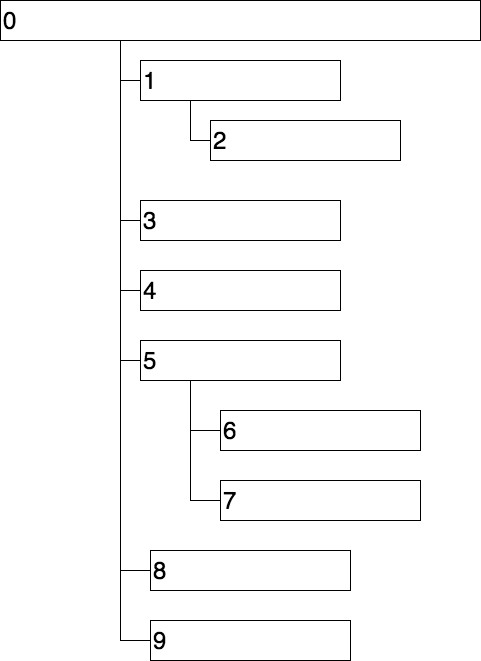
\includegraphics[width=0.5\textwidth]{../images/2.Related_Work/COLLAGREE_thread.png}
  \caption{COLLAGREEのスレッドの例}
  \label{Fig:thread1}
  \vspace{-10pt}
 \end{center}
\end{figure}

しかし,スレッドや返信は必ずしも正しく使われるとは限らず,単なるチャットと同様に扱われてしまいスレッドが乱立してしまうこともある.%今回の実験データをカウントする
図\ref{Fig:collagreeDiscuss}にCOLLAGREEでの実際の議論画面を示す.
\begin{figure}[htbp]
 \begin{center}
 \caption{COLLAGREEの議論画面}
  
\includegraphics[width=\textwidth]{../images/2.Related_Work/COLLAGREE_Discuss-min.png}
  %\caption{COLLAGREEの議論画面}
  \label{Fig:collagreeDiscuss}
  \vspace{-10pt}
 \end{center}
\end{figure}

図\ref{Fig:collagreeDiscuss}の上部の投稿フォームより,参加者は意見を自由に投稿することができる.投稿された意見は図\ref{Fig:collagreeDiscuss}の下部に表示され,参加者は各意見に対して返信や賛同を行うことができる.返信を繰り返すことでスレッドが構成され,図\ref{Fig:collagreeDiscuss}では3層のスレッドが構成されている.
%
COLLAGREE上での議論を支援する先行研究として,Itoら\cite{discSupport1-1}はCOLLAGREE上インセンティブとして参加者の活動の活発化や,重要投稿の把握の支援を目的に議論ポイントと呼ばれるシステムを導入した.システムでは参加者の投稿や投稿に対する返信や賛同に沿ってポイントを参加者に付与する.
また,高橋ら\cite{discSupport1-2}は質の高い投稿を促すために,議論ポイントを発展させて投稿された意見の質を評価する手法を提案した.投稿された意見中の名詞と以前に出現したキーワードとの一致度を計算し,一致していれば議論を収束させるものとして,一致していなければ議論を発散させるものとしてポイントを与える.
他に議論の可視化支援として,仙石ら\cite{argTree}は議論内容把握支援,合意形成支援,およびファシリテーション支援を目的として議論ツリーの実装を行った.ツリー図をCOLLAGREE に応用したものを仙石らが呼んだもので,ツリー図とはファシリテーターが参加者に議論のポイントと各意見の関係を一致させるために,参加者の意見を文字や図形を用いて分かりやすく描く図の1つである.図\ref{Fig:argTree1}に議論ツリーの例を示す.
\begin{figure}[htbp]
 \begin{center}
  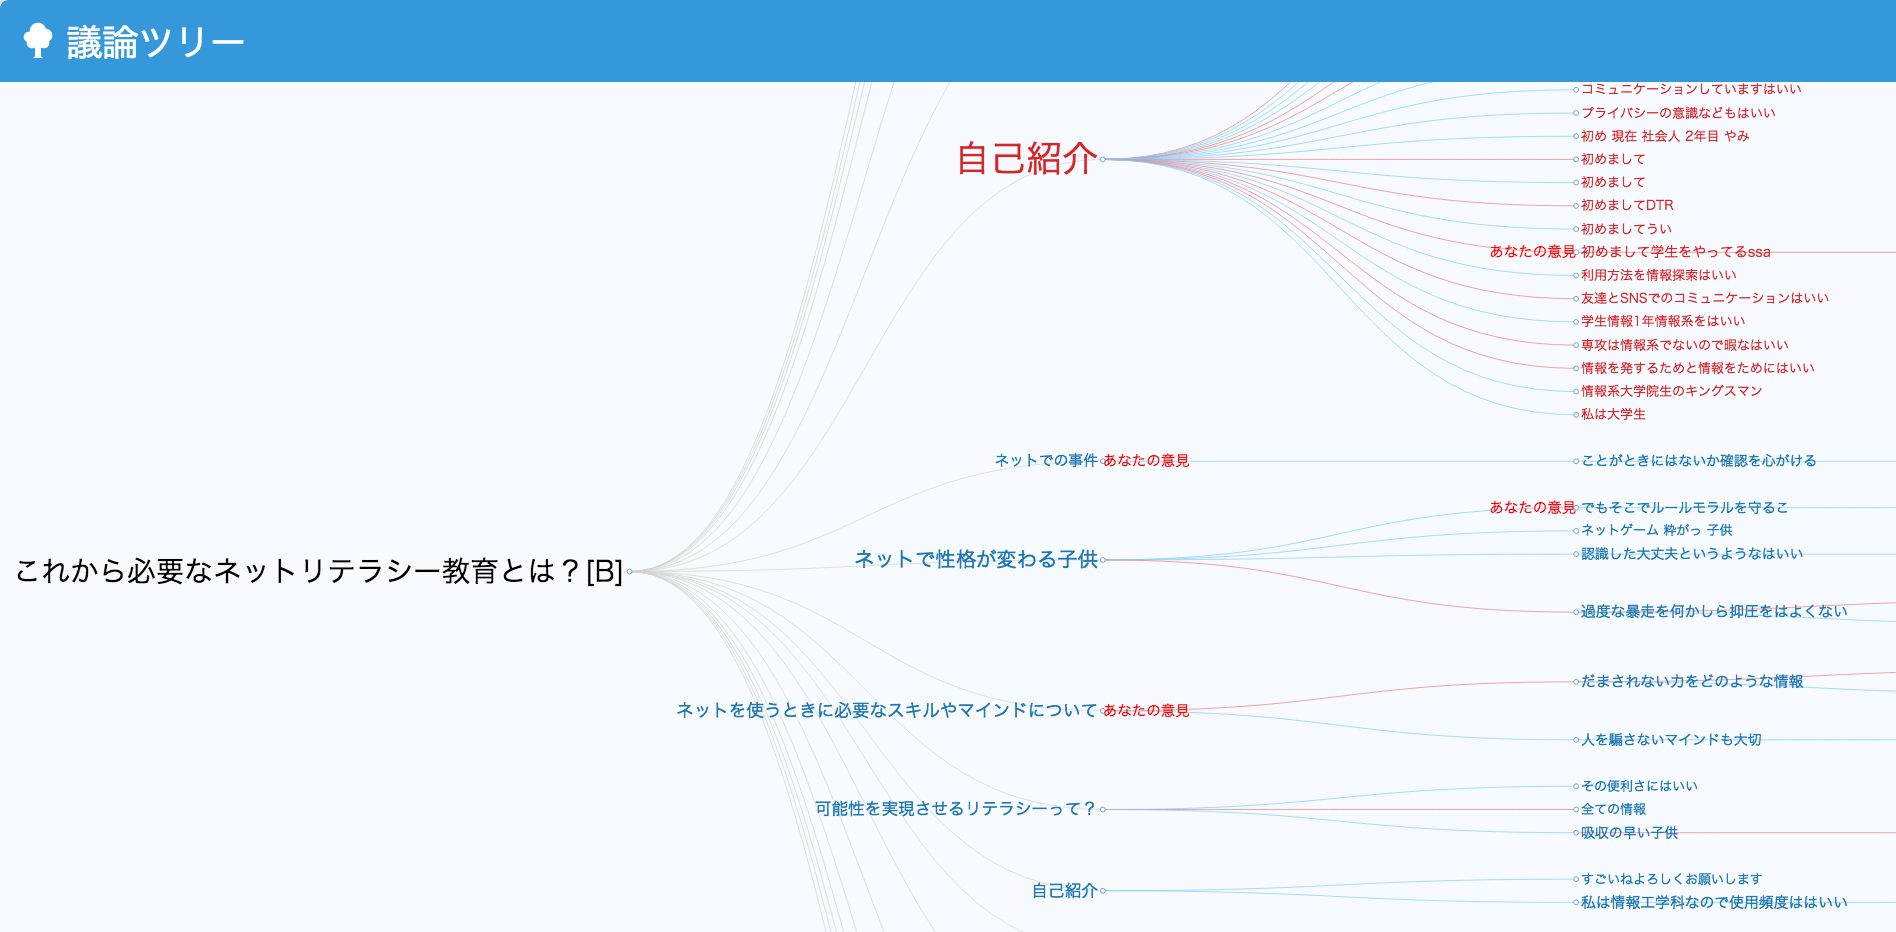
\includegraphics[width=\textwidth]{../images/2.Related_Work/argTree1.png}
  \caption{議論ツリー}
  \label{Fig:argTree1}
  \vspace{-10pt}
 \end{center}
\end{figure}
議論ツリーは投稿をノードとし,エッジは基本的に投稿間の返信関係を基に自動的に作られる.そして,より正確な議論ツリーを作成するためにファシリテーターが手動で議論ツリー編集するというハイブリッド方式が導入されている.

\subsection{ファシリテーター}
COLLAGREEではファシリテーターと呼ばれる人物が議論のマネジメントを行っている.
ファシリテーターは"促進者"を意味し,議論そのものには参加せず、あくまで中立的な立場から活動の支援を行うようにし,自分の意見を述べたり自ら意思決定をすることはない.
ファシリテーターの基本的な役割として"議論の内容の整理","議論の脱線防止","意見の促し"等が挙げられる.
%伊藤ら\cite{facilitation}によってファシリテーターの存在や手腕が合意形成に強く影響を与えることが示されている.
伊藤ら\cite{facilitation}や伊美ら\cite{collagree_Experiment}によってファシリテーターが様々な論点に対して発言を促し議論を発散させることで十分な議論が行われ,ファシリテーターの存在や手腕が合意形成に強く影響を与えることやWeb上での議論においてファシリテーターが有用であることが示されている.

%ファシリテーターの意見の促しが投稿数に繋がる.様々な論点に対して発言を促すことでそれぞれの論点に対する投稿に繋がる%(P5,6,7)
%@@@@@@@@@@@@@@@@@@@@@@@@@@@@@@@@@@@@
\section{議論支援}
\label{rel:argSupport}
\ref{rel:collagree:bg}節で述べたように近年大人数による議論には注目が集まっており,COLLAGREE以外でも議論内容の把握支援を行い,議論の進行を支援するための研究が行われている.
小谷ら\cite{discSupport2}は好意的発言影響度を取り入れた議論支援システムを開発した.システムは議論中の発言の意図や内容に加えて,発言に対するリアクション(同意、非同意、意見)などから議論進行をモニタリングしている.モニタリングの結果を基にして議論の活性化や深化に対して参加者が果たしている役割を"好意的発言影響度"として定量化して表示する.
以上を踏まえて,本研究と小谷らの開発した議論支援システムとの関連性と相違点について述べる.
両研究とも発言が議論に与える影響を扱っている点で関連している.しかし,小谷らは一般参加者や学習者の議論活性化及び収束に向けた支援を目的としているが,本研究はファシリテーターに対する支援を目的としている点で異なる.
%@@@@@@@@@@@@@@@@@@@@@@@@@@@@@@@@@@@@@
\section{話題遷移検出}
\label{rel:topic}
話題に関連する研究は1960年代に「会話分析」という学問から始まったとされる.
会話分析は会話を始めとする相互行為の組織(構造)を明らかにしようとする社会学の研究分野であり,相互行為の分析法を取り扱う.1960年代に Harvey Sacks と Emanuel A.schegloff によって創案された\cite{convAnalysis}.
%
話題は本来流れの一時点で簡単に区切ることのできるものではない.しかし,筒井\cite{zatsudan}は会話内容を分析する上で,連鎖組織及び言語形式との関連に基づいて分析を行っている.以下に筒井が立てた話題を区切る基準を1から5に示す.
\begin{enumerate}
  \item それまで話題となっていた対象や事態とは異なる,新しい対象や事態への言及\label{enum:zatsudan1}
  \item すでに言及された対象や事態の異なる側面への言及
  \item すでに言及された対象や事態の異なる時間における様相への言及
  \item すでに言及された対象や事態について,それと同種の対象や事態への言及
  \item すでに言及された個別の対象や事態の一般化\label{enum:zatsudan5}
\end{enumerate}
本研究では上記の基準を参考に話題変化の判定の評価の基準を設けている.

話題の遷移に基づいた文章の分割は人間によるテキスト全体の内容の把握の容易化や複数のテキストに対する自動分類や検索の精度向上のために研究されている.以下では話題の遷移に関する関連研究について述べる.
\subsection{テキストセグメンテーション}
テキストセグメンテーションは複数のトピックが混合的に書かれている非構造的である文書をトピックに応じて分割する手法である.
\paragraph{TextTiling}\ \\
Hearstら\cite{texttiling}は複数の単語を連結した2つのブロックをテキストの初めから末尾まで動かしていきブロック間の類似度を計算する手法(TextTiling,Hearst法とも呼ばれる)を提案した.類似度はブロック間で共通して使われる単語数などで計算する.図\ref{Fig:textTilingFigure}に手法の簡単な流れを示す.
\begin{figure}[htbp]
 \begin{center}
  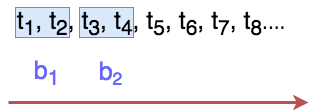
\includegraphics[width=\textwidth]{../images/2.Related_Work/textTiling-figure.png}
  \caption{TextTilingの流れ}
  \label{Fig:textTilingFigure}
  \vspace{-10pt}
 \end{center}
\end{figure}

計算された類似度をグラフにすると図\ref{Fig:textTilingGraph}のようになる.縦軸はブロック間の類似度,横軸はブロック間の番号を表し,グラフ中の番号は段落番号,垂直線は選出された文の境界位置を表す.グラフは各ブロック間の類似度を繋いだものと,更に平滑化したものの2つが描かれている.
グラフの谷のような場所は左右のブロック間の類似度が下がる場所を表している.類似度が下がることは使われる単語が変わったこと,すなわちトピックが変わったことを意味しており,谷の付近に境界を設けることで文書をトピックごとに区切ることを可能としている.
\begin{figure}[htbp]
 \begin{center}
  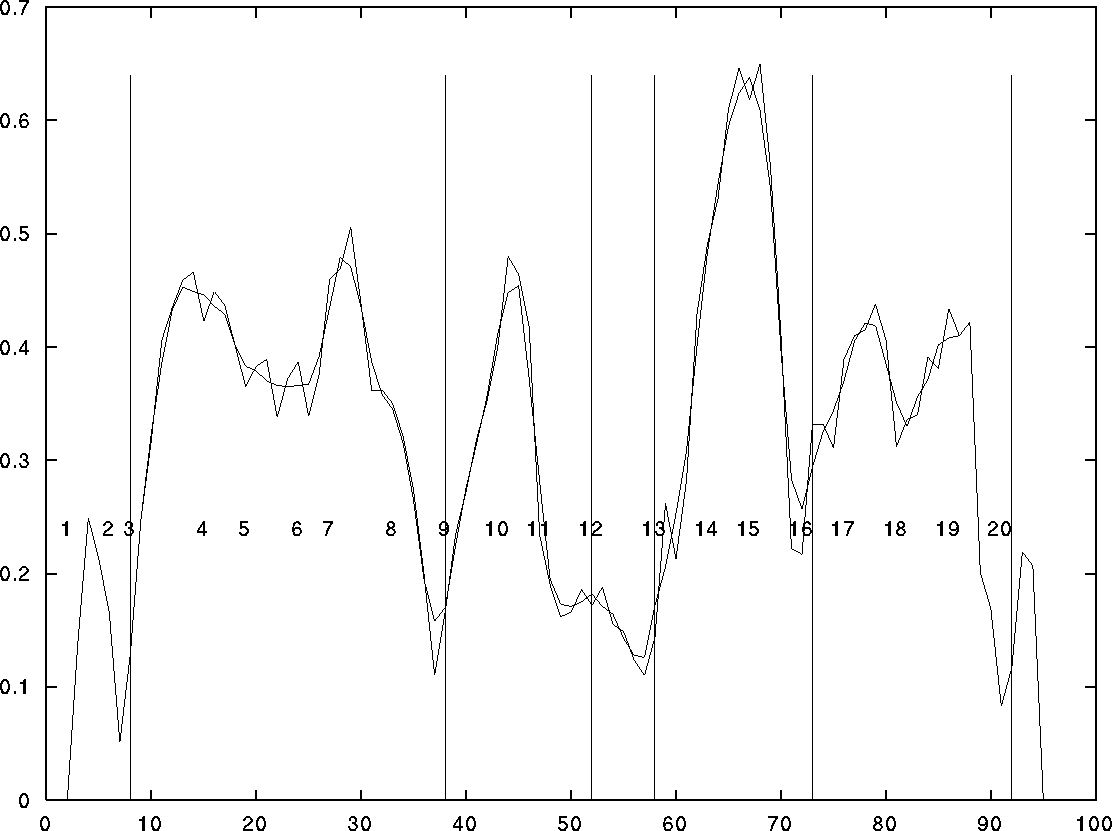
\includegraphics[width=\textwidth]{../images/2.Related_Work/textTiling-graph.png}
  \caption{TextTilingのグラフ}
  \label{Fig:textTilingGraph}
  \vspace{-10pt}
 \end{center}
\end{figure}

\paragraph{テキストセグメンテーションを使用した関連研究}\ \\
別所\cite{textSegmentation1}は単語の共起頻度行列を特異値分解で次元を削減して作成した単語の概念ベクトルを用いて,連結された新聞記事を元の形になるように分割をする実験を行っている.TextTilingを用いてブロック間の類似度を計算する際にブロック中の単語の中で自立語にのみ概念ベクトルを付与し,左右のブロックの和ベクトル(または重心ベクトル)の余弦測度を求め,類似度(または結束度)としている.

以上を踏まえて,本研究とテキストセグメンテーションを用いた研究との相違点について述べる.
テキストセグメンテーションは基本的にある地点$A$で話題に沿って分割をするか考える際に,地点$A$より先の情報を使うことができる.すなわち,ある程度の文章が現れてから話題が変わったかどうかの判定をしており,リアルタイムでの動作を想定していない.
本研究はリアルタイムでの動作を想定し,ある発言$B$が話題の変化を起こすかどうか判定する際に$B$より先の情報を使うことなく判定している点で異なる.
%
\subsection{トピックモデル}
トピックモデル\cite{topicModel}は確率モデルの一種にあたり,文章中の「単語が出現する確率」を推定している.単語が出現する確率をうまく推定することができれば,似たような単語が出てくる文章が把握できる.
すなわち,トピックモデルとは「文書における単語の出現確率」を推定するモデルといえる.
\paragraph{ユニグラムモデル}\ \\
%図は四角の箱が文書を表し,中身の色がトピックを表す.
%ユニグラムモデルは,すべてのボックスが同じ青色である.全ての文書の単語は,一つのトピックから生成されたものと仮定するモデルである.
ユニグラムモデルは,全ての文書の単語は,一つのトピックから生成されたものと仮定するモデルである.
以下の図\ref{Fig:unigram},図\ref{Fig:mixUnigram},図\ref{Fig:LDA}は四角の箱が文章を表し,中身の色がトピックを表しているとしてユニグラムモデルについて述べる.図\ref{Fig:unigram}で示されているユニグラムモデルは文章であるすべてのボックスが同じ色の状況を示している.すなわち,全ての文書の単語は1つのトピックから生成されたと仮定するモデルである.
\begin{figure}[htbp]
 \begin{center}
  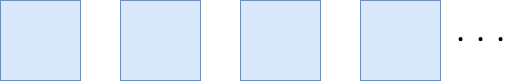
\includegraphics[width=\textwidth]{../images/2.Related_Work/topicModel-unigram.png}
  \caption{ユニグラムモデル}
  \label{Fig:unigram}
  \vspace{-10pt}
 \end{center}
\end{figure}
\paragraph{混合ユニグラムモデル}\ \\
図\ref{Fig:mixUnigram}で示されている,混合ユニグラムモデルは各ボックスの色が異なっている.つまり,各文書に一つのトピックがあり,該当するトピックから文書の単語が生成されると仮定するモデルである.
\begin{figure}[htbp]
 \begin{center}
  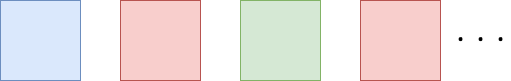
\includegraphics[width=\textwidth]{../images/2.Related_Work/topicModel-mixUnigram.png}
  \caption{混合ユニグラムモデル}
  \label{Fig:mixUnigram}
  \vspace{-10pt}
 \end{center}
\end{figure}
\paragraph{LDA}\ \\
図\ref{Fig:LDA}で示されている,LDA(Latent Dirichlet Allocation)\cite{LDA2003}では,ボックスの中で色が異なっている.つまり,各文書は複数のトピックで構成されていて,各トピックの単語分布を合算した形で単語が生成されていると仮定を行うモデルである.
\begin{figure}[htbp]
 \begin{center}
  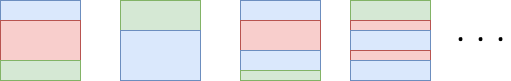
\includegraphics[width=\textwidth]{../images/2.Related_Work/topicModel-LDA.png}
  \caption{LDA}
  \label{Fig:LDA}
  \vspace{-10pt}
 \end{center}
\end{figure}

LDAでは文書$d$中のトピック$t$の単語の割合$p(t|d)$とトピック$t$で単語$w$が生成される確率$p(w|t)$を学習データとの誤差が小さくなるように学習していく.

\paragraph{トピックモデルを使用した関連研究}\ \\
中村ら\cite{topicLDAshift}は連結された新聞記事をLDAを用いてトピック変化点を検出して分割する実験を行った.
中村らが行ったトピック変化点を検出する手順を図\ref{Fig:LDA-topicFlow}に示す.
\begin{figure}[htbp]
 \begin{center}
  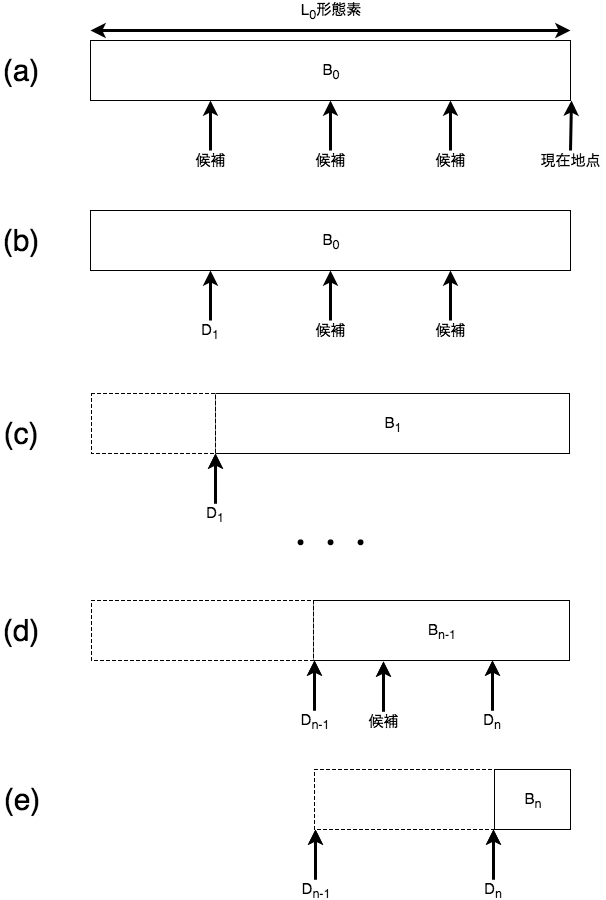
\includegraphics[width=\textwidth]{../images/2.Related_Work/LDA-topicFlow.png}
  \caption{トピック変化点検出手順}
  \label{Fig:LDA-topicFlow}
  \vspace{-10pt}
 \end{center}
\end{figure}

\begin{enumerate}
  \item 現在地点より前の$L_0$個の形態素を処理対象範囲$B_0$とし($L_0>L;L=文章長の下限$),$B_0$から複数のトピック変化点候補箇所を抽出する.図\ref{Fig:LDA-topicFlow}(a)に該当する.
  \item $B_0$を各トピック変化点候補箇所で2ブロックに分割し,2ブロック間の類似度を計算する.そして類似度が最も小さくなるトピック変化点候補箇所$D_1$とその類似度$S_1$を求める.文書ブロック間の類似度はLDAによって求められるブロックのトピック混合比ベクトルを用いて算出する.図\ref{Fig:LDA-topicFlow}(b)に該当する.
  \item $B_0$を$D_1$で分割し,現在地点に近い側のブロックを$B_1$とする.図\ref{Fig:LDA-topicFlow}(c)に該当する.
  \\
  以降は以下4.と5.の処理を繰り返す($n\geq2$).
  \item ブロック$B_{n-1}$に対し2.と同様の手順でトピック変化点候補箇所$D_n$とその類似度$S_n$を求める.図\ref{Fig:LDA-topicFlow}(d)に該当する.
  \item $S_n \geq S_{n-1}$の場合,$D_{n-1}$をトピック変化点として処理を終了する.$S_n <  S_{n-1}$の場合,$B_{n-1}$を$D_n$で分割し現在地点に近い側のブロックを$B_n$として,処理を継続する.図\ref{Fig:LDA-topicFlow}(e)に該当する.
\end{enumerate}
なお,上記1.におけるトピック変化点候補は1文中でトピックが変化することは考えにくいことと計算コストを考慮し,文境界(句点出現位置)をトピック変化点候補としている.

以上を踏まえて,本研究とトピックモデルを用いた研究との相違点について述べる.
トピックモデルはトピックに基づいて学習を行っていて,基本的に学習の際にトピックの数を指定する必要があり,指定に伴いトピック数が制限されてしまう.また,教師なし学習であるので必ずしも話題を捉えた学習がされるとは限らない.すなわち,トピックの数によっては変化に対応できない話題が存在することがあり得る.本研究はトピックの指定が必要なLDAによるトピックモデルとは違い,トピックに関係なく単語の共起頻度を学習するfastTextを用いている点で異なる.
更に,本研究は中村らの研究とは話題の変化点を判定する際に複数候補から類似度が最小である点を選ぶのではなく,候補を逐一調べ閾値を下回るかどうかで変化点を判定している点でも異なる.
%@@@@@@@@@@@@@@@@@@@@@@@@@@@@@@@@@@@@@@@@
\section{重み付け}
\label{rel:part:weight}
重み付けは情報検索を主とする分野で使われる方法で,蓄積された情報中の語の索引語,すなわち特定の情報の特徴を表し検索の手掛かりとなる語,としての重要度を数値的に表現し,それぞれの語の重要度に応じて重みを付け,集計して総合評価を出す手法である.出された総合評価はスコア等と呼ばれる.一般的に語の重要度は整数または実数値で与えられる.自動的な重み付けにおいては語の出現頻度情報や出現位置を利用して数値を与える.
本研究で行う重み付けは下記の2種類の重み付けを基にしている.
\subsection{Okapi BM25}
Okapi BM25\cite{okapiBM25} は出現頻度情報を用いる重み付け手法の代表の1つである.Okapi BM25 ではTF(Term Frequency 単語の出現頻度)\cite{tf},IDF(Inverse Document Frequency 逆文書頻度)\cite{idf},DL(Document Length 文書長)の3つを用いて重要度の計算を行う.
各用語について説明を行う.
\paragraph{TF}\ \\
TFは単語の出現頻度を表し,文書中において出現頻度の高い単語は重要であるという考え方に基づく.ある単語$t_i$の文書$D_j$中における出現頻度重み$tf_{i,j}$は式(\ref{eq:tf})のようにして求められる.
\begin{equation}
\begin{aligned}
\label{eq:tf}
tf_{i,j} & = \frac{n_{ij}}{ \sum_{k} n_{kj} }
\end{aligned}
\end{equation}
ここで$n_{ij}$は文書$d_{j}$における単語$t_{i}$の出現回数,$\sum _{k} n_{kj} $は文書$d_{j}$におけるすべての単語の出現回数の和である.
\paragraph{IDF}\ \\
IDFは逆文書頻度を表し,多くの文書において出現頻度の高い単語は重要ではないという考え方に基づく.IDFは多くの文書に出現する語,すなわち一般的な語の重要度を下げ,特定の文書にしか出現しない単語の重要度を上げる役割を果たす.ある単語$t_i$の逆文書頻度重み$idf_{i}$は式(\ref{eq:idf})のようにして求められる.
\begin{equation}
\begin{aligned}
\label{eq:idf}
idf_{i} & = \log{ \frac{ |D| }{ | \{ d: d \ni t_i \}  |} } %+1は本研究ではしない
\end{aligned}
\end{equation}
ここで$|D|$は総文書数,$| \{ d: d \ni t_i \}  |$は単語$t_i$を含む文書数である.
\paragraph{DL}\ \\
DLは文書長を表し,ある単語の出現回数が同じ2つの文書について,総単語数の少ない文書と多い文書では,前者のほうがより価値があるという考え方に基づく.
ある文書$d_j$の文書長重み$ndl_j$は式(\ref{eq:dl})のようにして求められる.
\begin{equation}
\begin{aligned}
\label{eq:dl}
ndl_{j} & = \frac{dl_j}{ave(dl)}
\end{aligned}
\end{equation}
ここで$dl_j$は文書$d_j$の総単語数,$ave(dl)$はすべての文書の平均$dl$を表す.
%Okapi BM25
\\
上記の3つの重みを用いてOkapi BM25は(\ref{eq:bm25})のように単語$t_i$の文書$D_j$中における統合重み$cw_{ij}$を求める.
\begin{equation}
\begin{aligned}
\label{eq:bm25}
cw_{ij} & = \frac{tf_{i,j} \cdot idf_{i} \cdot (k_1+ 1)}{k_1 \cdot (1 - b + b \cdot ndl_{j}  ) + tf_{i,j}  }
\end{aligned}
\end{equation}
ここで定数$k_1$と$b$について説明する.2つの定数はどちらもチューニングの役割を果すもので$k_1$は単語の出現頻度による影響を,$b$は文書の長さによる影響を調節する.
\subsection{LexRank}
Erkanら\cite{lexRank}によって考案されたLexRankはGoogleのPageRank\cite{pageRank1999}を使用した文章要約アルゴリズムで,文の類似度を計算して次の2つの基準に基いて文の重要度を計算する.
\begin{enumerate}
  \item 多くの文に類似する文は重要な文である.
  \item 重要な文に類似する文は重要な文である.
\end{enumerate}
LexRankでいう類似度は簡単にいえば2文がどれだけ共通の単語を持つかということを表し,文をTF-IDFを用いてベクトル化してCosineを求めることで類似度としており,式\ref{eq:cosine}に沿ってベクトル$x$と$y$のCosineが計算される.
\begin{equation}
\begin{aligned}
\label{eq:cosine}
{\rm idf-modified-cosine}(x,y) & = \frac{\sum_{w \in x,y} tf_{w,x} tf_{w,y} (idf_w)^2} {\sqrt{ \sum_{x_i \in x} ( tf_{x_i,x} idf_{x_i} )^2  } \times \sqrt{ \sum_{y_i \in y} ( tf_{y_i,y} idf_{y_i} )^2  }}
\end{aligned}
\end{equation}

文の間のCosine類似度をグラフとして可視化すると図\ref{Fig:lexGraph1}のようになる.各エッジは文の間のCosine類似度を表し,$dXsY$は文書XのY番目の文を示す.
\begin{figure}[htbp]
 \begin{center}
  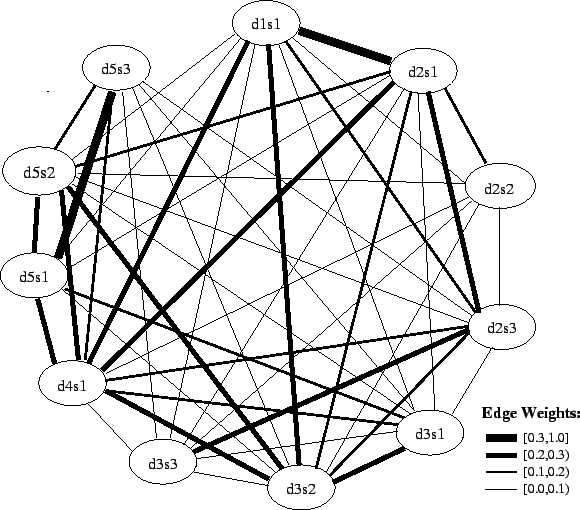
\includegraphics[width=\textwidth]{../images/2.Related_Work/lexRank-graph.png}
  \caption{類似度グラフの例}
  \label{Fig:lexGraph1}
  \vspace{-10pt}
 \end{center}
\end{figure}

その後,Cosine類似度が閾値を超えたかどうかを基に隣接行列が作成される.隣接行列はグラフを表現するために用いられる行列で,あるノード$v$と$w$の間にエッジの有無が行列の$(v,w)$成分に割り当てられる.
隣接行列の各要素を類似している文の数で割り,確率行列に変換した後,\textbf{Algorithm\ref{algo:powMethod}}に従って行列の固有ベクトル$\bm{p}$が計算される.求められた固有ベクトルがLexRankスコアとなる.
\begin{algorithm}
\caption{べき乗法の計算アルゴリズム} \label{algo:powMethod}
\begin{algorithmic}[1]
\State Input : 確率的かつ既約かつ非周期的な行列$\bm{M}$
\State Input : 行列サイズ $N$, 誤差許容値$~ \epsilon$
\State Output: 固有ベクトル $\bm{p}$
\Procedure{powerMethod}{$M,N,\epsilon$} 
	\State $\bm{p}_{0}=  \frac{1}{N} \bm{1};$
	\State $t=0;$
	\Repeat
		\State $t=t+1;$
		\State $\bm{p}_{t} = \bm{M}^{\mathrm{T}} \bm{p}_{t-1};$
		\State $\delta = \| \bm{p}_{t} - \bm{p}_{t-1} \| ;$
	\Until $ \delta < \epsilon$
	\State \textbf{return} $\bm{p}_{t};$
\EndProcedure
\end{algorithmic}
\end{algorithm}

LexRankスコアを計算する一連のアルゴリズムを\textbf{Algorithm\ref{algo:lexRank}}に示す.
\begin{algorithm}
\caption{LexRankスコアの計算アルゴリズム} \label{algo:lexRank}
\begin{algorithmic}[1]
\State $Input: n 個の文からなる配列 S, コサイン類似度の閾値 threshold$
\State $Output: 各文のLexRankスコアを格納した配列L$
\State $Array ~~ CosineMatrix[n][n];$
\State $Array ~~ Degree[n];$
\State $Array ~~ L[n];$
\Procedure{LexRank}{$S,t$} 
	 \For{$i \gets 1 ~  to  ~ n $}\label{algo:lexRank:for1-b}
	 	\For{$j \gets 1 ~ to ~ n $}\label{algo:lexRank:for2-b}
			\State $CosineMatrix[i][j]$ = idf-modified-cosine$(S[i], S[j]);$\label{algo:lexRank:cos}
			\If{$CosineMatrix[i][j] > threshold $}
				\State $CosineMatrix[i][j] = 1;$
				\State $Degree[i]++;$
			\Else
			 	\State $CosineMatrix[i][j] = 0;$
			\EndIf
		\EndFor\label{algo:lexRank:for2-e}
	 \EndFor\label{algo:lexRank:for1-e}
        \For{$i \gets 1 ~ to ~ n$}\label{algo:lexRank:for3-b}
    		\For{$j \gets 1 ~ to ~ n$}\label{algo:lexRank:for4-b}
         		\State $CosineMatrix[i][j] = CosineMatrix[i][j] / Degree[i];$
    		\EndFor\label{for4}\label{algo:lexRank:for4-e}
	\EndFor\label{for3}\label{algo:lexRank:for3-e}
	\State L = PowerMethod$(CosineMatrix, n, ε);$\label{algo:lexRank:pw}
	\State \textbf{return} L
\EndProcedure
\end{algorithmic}
\end{algorithm}

\ref{algo:lexRank:for1-b}$\sim$\ref{algo:lexRank:for1-e}行目では隣接行列が作成されており,\ref{algo:lexRank:for3-b}$\sim$\ref{algo:lexRank:pw}行目ではLexRankが計算されている.
%また,LexRankには Continuous LexRank が存在し,9行目の閾値がない
%@@@@@@@@@@@@@@@@@@@@@@@@@@@@@@@@@@@@@@@
\section{分散表現}
\label{rel:part:vec}
自然言語処理では単語を低次元または高次元の実数ベクトルで表現する技術でHarris\cite{firth1957hypothesis}が提唱した"分布仮説"("同じ文脈で出現する単語は類似した意味を持つ傾向があり,単語はその単語とともに出現する単語等によって特徴づけられる."という考え方)に基づいている.
\subsection{単語文脈行列}
\label{rel:wordEmbed:WordParagraphMat}
単語文脈行列は分散表現の最も基本的な形式で図\ref{Fig:WordParagraphMat}のような形の行列で表される.
\begin{figure}[htbp]
 \begin{center}
  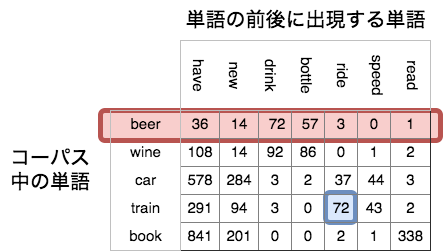
\includegraphics[width=\textwidth]{../images/2.Related_Work/WordParagraphMatrix2.png}
  \caption{単語文脈行列( https://www.slideshare.net/naoakiokazaki/20150530-jsai2015 の表を筆者修正)}
  \label{Fig:WordParagraphMat}
  \vspace{-10pt}
 \end{center}
\end{figure}

行列中の各要素$M_{ij}$は単語$i$と文脈$j$の共起頻度を表しており,例として青い四角はtrainとrideが72回共起したことを表している.各行$M_i$は単語$i$の意味ベクトルを表し,例として赤い四角は"beer"の単語ベクトルを表している.
また,単語の類似度を式\ref{eq:cosineSim}のように単語の意味ベクトルのコサイン類似度で求めることができる.
\begin{equation}
\begin{aligned}
\label{eq:cosineSim}
cos \theta & = \frac{M_i \cdot M_j}{ | M_i | | M_j |}
\end{aligned}
\end{equation}

式\ref{eq:cosineSim}を図\ref{Fig:WordParagraphMat}の行列に適応させるとbeerとwineのコサイン類似度は約$0.941$,beerとtrainのコサイン類似度は約$0.387$となり,trainよりもwineの方がbeerに類似していることが分かる.
%また後述のword2vecやfastTextでは他の数学的処理が可能となるが,分散表現は問題点として類義語と対義語を区別できないことが挙げられる.
\subsection{word2vec}
\ref{rel:wordEmbed:WordParagraphMat}節で説明した単語文脈行列から得られる単語ベクトルは単語の類似度を求めることは出来たが,他の数学的処理には対応していなかった.
%word2vecは単語文脈行列とは異なり予測することで学習する
Mikolovら\cite{word2vec}が開発したword2vecはニューラルネットワークを用いて分散表現の生成を行う手法で,文脈または単語を予測するようにニューラルネットワークで学習を行い,隠れ層をベクトルとする.
具体的にはword2vecで使用される学習方法にはCBOWとskip-gramの2種類が存在する.図\ref{Fig:CBOW},図\ref{Fig:skip-gram}はそれぞれCBOWとskip-gramの構造を表す.
\begin{figure}[htbp]
	\begin{center}
	\begin{tabular}{c}
      	% 1
      		\begin{minipage}{0.5\textwidth}
       		 \begin{center}
 	 		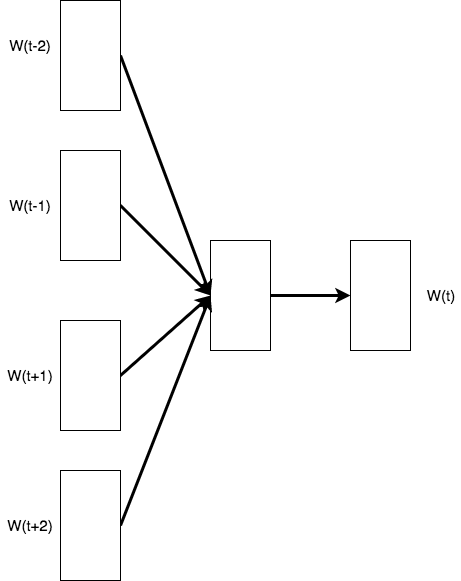
\includegraphics[width=\hsize]{../images/2.Related_Work/CBOW.png}
  			\caption{CBOW}
 	 		\label{Fig:CBOW}
 		 	\vspace{-10pt}
 		\end{center}
		\end{minipage}
	% 2
      		\begin{minipage}{0.5\textwidth}
       		 \begin{center}
 	 		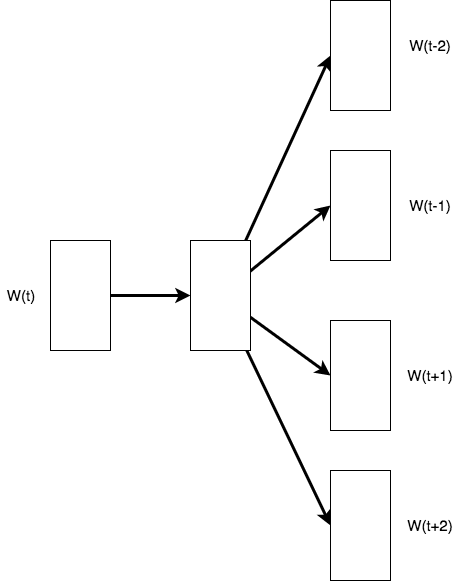
\includegraphics[width=\hsize]{../images/2.Related_Work/skip-gram.png}
  			\caption{skip-gram}
 	 		\label{Fig:skip-gram}
 		 	\vspace{-10pt}
 		\end{center}
		\end{minipage}
	\end{tabular}
	 \end{center}
\end{figure}

CBOWは周辺の単語$W(t-2) \cdots  W(t+2)$を入力として,現在の単語$W(t)$を予測することを目指して学習する.逆にskip-gramは現在の単語を入力として,周辺の単語を予測することを目指して学習する.どちらの手法でも中間層と単語の変換処理が行われており,学習によって得られる単語と中間層での数値が対応した行列が単語の分散表現モデルとなる.

word2vecが従来の手法と比べて大きく異なる点は ニューラルネットによる学習で単語の類似度の計算に加えて,ベクトルの加減算が単語の意味の加減算に対応しているということである.また,従来の手法を用いた単語ベクトルよりも類推精度が高いことがLevyら\cite{levy2014neural}によって示されている.
例えば,$X=vector("biggest") - vector("big") + vector("small")$として計算されたベクトル$X$に最も類似したベクトルを探すことでbiggestがbigに類似しているのと同じ意味でsmallに類似している単語smallestを見つけることができる.ただし,分散表現モデルが十分に訓練されていることが前提である.

\subsection{fastText}
fastText\cite{fastText}\cite{fastText2}はword2vecを発展させた手法でより大きな語彙や多くの稀な単語に対応することができ,学習の速度を上昇させることにも成功している.

fastTextはskip-gramモデルを採用しており,学習の際に単語だけでなく部分語(単語を構成する文字のまとまり)についても考慮する.以下に単語$w_t$が与えられた時に予測した文脈単語$w_c$の間のスコア関数を示す.
\begin{equation}
\begin{aligned}
\label{eq:para_scoreF_1}
s(w_t , w_c) & = \bm{ u }^{\mathrm{T}}_{w_t} \bm{v}_{w_c}
\end{aligned}
\end{equation}

\begin{equation}
\begin{aligned}
\label{eq:para_scoreF_2}
s(w_t , w_c) & =  \sum_{g \in \mathcal{G}_w} \bm{ z }^{\mathrm{T}}_{g} \bm{v}_{w_c}
\end{aligned}
\end{equation}

式\ref{eq:para_scoreF_1}はfastText以前の手法でのスコア関数を表し,式\ref{eq:para_scoreF_2}はfastTextでのスコア関数を表す.$\bm{u}_{w_{t}}$,$\bm{v}_{w_c}$はそれぞれ単語$w_t$,$w_c$を実数ベクトルで表したもので,式\ref{eq:para_scoreF_2}において$\mathcal{G}_w$,$\bm{z}_{g}$はそれぞれ単語$w$のn-gramの集合とn-gram $g$を実数ベクトルで表現したものを表す.
式\ref{eq:para_scoreF_1}では単語と文脈単語の間のスカラー積をスコアとしているが,式\ref{eq:para_scoreF_2}では単語のn-gramと文脈単語の間のスカラー積の合計をスコアとしている.
式\ref{eq:para_scoreF_2}の手法を用いることで従来のモデルでは考慮されていなかった"活用形"を考慮できるようになった.例として,単語 goとgoesとgoingは全てgoの活用形であるが字面は異なるので従来のモデルでは異なる単語として学習されていたが,fastTextでは部分語である"go"を3つ全てで学習することで意味の近しい単語として学習することが可能となることが挙げられる.

本研究では分散表現の手法としてfastTextを使用している.
\subsection{分散表現を使用した話題関連研究}
分散表現は関連語を導出できることから分散表現を話題関連に用いる研究が行われている.
中野ら\cite{embedTopic1}は分散表現を用いて雑談対話システムでのシステム側の応答生成を行っている.
図\ref{Fig:embedTopic1}に話題展開システムの構造を示す.
\begin{figure}[htbp]
 \begin{center}
  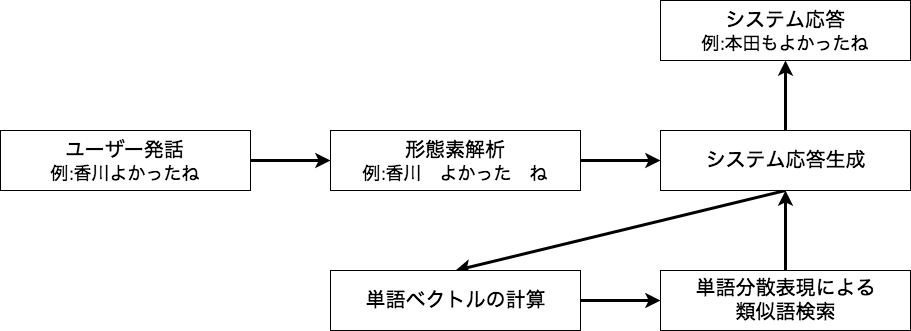
\includegraphics[width=\textwidth]{../images/2.Related_Work/embedTopic1.png}
  \caption{話題展開システムの構造}
  \label{Fig:embedTopic1}
  \vspace{-10pt}
 \end{center}
\end{figure}

システムではユーザ発話を形態素解析して検出された単語を単語分散表現による類似語検索から得られた結果と入れ替えることでシステム応答の生成を行っている.

また,Liら\cite{embedTopic2}は分散表現を用いてTwitterのツイートをトピックカテゴリに分類する分類器 TweetSift を提案している.
図\ref{Fig:embedTopic1}にトピックカテゴリの予測のワークフローを示す.
\begin{figure}[htbp]
 \begin{center}
  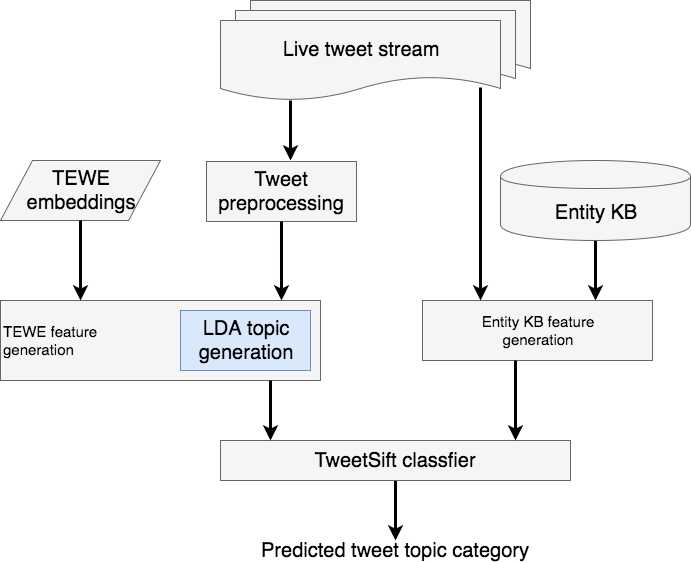
\includegraphics[width=\textwidth]{../images/2.Related_Work/TweetSift.png}
  \caption{TweetSiftによるトピック予測のワークフロー}
  \label{Fig:tweetSift}
  \vspace{-10pt}
 \end{center}
\end{figure}

図\ref{Fig:embedTopic1}の右のフローではツイートデータとスクレイピングで作成された知識ベースを用いて知識ベース特徴を生成している.
図\ref{Fig:embedTopic1}の左のフローでは前処理を行ったツイートと作成済み分散表現モデルを用いて分散表現特徴を生成している.
2つの特徴を用いてSMO(Sequential Minimal Optimization)\cite{SMO}によってトピックが予測されている.
Liらの研究で用いられる分散表現は学習の際に単語だけでなく,LDAを用いて予測した単語のトピックも使用されている.

以上を踏まえて,本研究と分散表現を用いた研究との相違点について述べる.
本研究はWeb上での議論を対象としており,対話やSNSを対象としていない点で異なる.また,中野らの研究とは文の生成を行わない点でも異なり,Liらの研究とは分散表現の学習の際にトピックを用いていない点でも異なる.

\section{結言}
\label{rel:conclusion}
本章では,COLLAGREEの開発の背景及び概要とCOLLAGREE上で既存の議論支援について説明し,本研究で支援することを目的とするファシリテーターについても説明した.
次に,既存の議論支援研究を紹介して本研究との相違点を説明した.
また,話題に関連する研究の概要と話題遷移を研究している点で本研究と関連している研究についても述べ,本研究との相違点を説明した.
そして,本研究での重要な要素である重み付けと分散表現についてと,分散表現を使用した関連研究について説明し,本研究との相違点を説明した.

 %-------------------------------------------------------------------------------
 \expandafter\ifx\csname MasterFile\endcsname\relax
	\def\BibFile{hoge}
	\expandafter\ifx\csname MasterFile\endcsname\relax
\def\SubFile{hoge}
\documentclass[a4j,12pt,twoside,openany]{jreport}
%\nofiles %tocファイルを更新させない
%\documentclass[12pt,a4j,twoside,openany]{jsbook}
\usepackage[dvipdfmx]{graphicx}
\usepackage{../dspc} % ベースラインスキップの指定
\usepackage{../slashbox} % 表に斜線を入れる
%\usepackage{../mediabb}
\usepackage{fancyvrb} % Verbatim環境
\usepackage{fancyhdr} % Headerの下線付き章見出し
\usepackage{here} % float[H]
\usepackage{multirow}
\usepackage{hhline} % 表の罫線の角を美しくする
\usepackage{amsmath} %コレがないとcasesが動かない
\usepackage{amsfonts} % 数学用フォント
\usepackage{bm} % 数式環境での bold
\usepackage{algorithm}
\usepackage{algorithmicx}
\usepackage[noend]{algpseudocode}%\procedureはここに含まれる
\usepackage[flushleft]{threeparttable} % 脚注付きテーブル
\usepackage{enumitem}
\usepackage{comment}
\usepackage{fancybox}
%\usepackage{csvsimple,booktabs,siunitx}
%\usepackage{filecontents}
\usepackage{ulinej}


\setlength{\evensidemargin}{5pt}
\setlength{\oddsidemargin}{40pt}
%\setlength{\headheight}{16.5pt}
%%\setlength{\headheight}{30pt}
\setcounter{secnumdepth}{3}
\setlist[description]{leftmargin=2\parindent,labelindent=\parindent}

\makeatletter
\def\@makechapterhead#1{%
	\vspace*{50\p@}%
	{
		\parindent \z@ \raggedright \normalfont
		\ifnum \c@secnumdepth >\m@ne
		% \if@mainmatter
			\huge\bfseries\@chapapp\thechapter\@chappos
			\par\nobreak
			\vskip 20\p@
		% \fi
		\fi
		\interlinepenalty\@M
		\Huge\bfseries #1\par\nobreak
		\vskip 40\p@
	}
}

%新しいコマンド定義
\newcounter{linenumber}
\newenvironment{listing}{%
  \begin{list}{%
    \small\arabic{linenumber}:}{%
      \usecounter{linenumber}%
      \setlength{\baselineskip}{18pt}%
      \setlength{\itemsep}{0pt}%
      \setlength{\parsep}{0pt}}}%
 {\end{list}}
\newcommand{\figcaption}[1]{\def\@captype{figure}\caption{#1}}
\newcommand{\tblcaption}[1]{\def\@captype{table}\caption{#1}}
\newcommand{\norm}[1]{\left\| #1 \right\|}
\newcommand{\cc}[1]{\multicolumn{1}{|c|}{#1}}
\newcommand{\circled}[1]{\raisebox{.5pt}{\textcircled{\raisebox{-.9pt} {#1}}}}
\newcommand{\specialcell}[2][c]{%
  \begin{tabular}[#1]{@{}c@{}}#2\end{tabular}}
\makeatother
%===============================================================================
\expandafter\ifx\csname SubFile\endcsname\relax
\begin{document}
\def\MasterFile{hoge}
%-------------------------------------------------------------------------------
%\maketitle
\thispagestyle{empty}
\documentclass[a4j,12pt]{jarticle}
% 外表紙

% 題名
\def\title{降水量予測のための\\Sequence-to-Sequenceモデルに基づく\\マルチモーダル学習}
% 著者
\def\author{林 政行}
% 入学年度(平成)
\def\year{24}
% 学籍番号
\def\number{24115113}
% 指導教官
\def\kyoukan{伊藤孝行}
% 指導教官役職
\def\kyoukanrank{教授}
% 提出日
\def\teisyutubi{平成28年2月8日}

\begin{document}
\pagestyle{empty}
\baselineskip=18pt

\begin{center}

\vspace*{2cm}

{\huge \textbf{卒業論文}}

\vspace*{3cm}

%\vrule width 10cm height 1pt depth 0pt



%(題目)
%\vspace{5pt}
%\hrule height 3pt
%\vspace{1zh}

\vrule width 6.25cm height 6pt depth -2pt
\makebox[1.5cm]{(題目)}
\vrule width 6.25cm height 6pt depth -2pt

{\LARGE {\title}}

\vspace{1zh}
%{\large {\subtitle}}
%\hrule height 3pt
\vrule width 14cm height 4pt depth 0pt

\vspace*{1cm}

指導教員 {\large {\kyoukan}} {\kyoukanrank}

%\vspace*{5cm}
\vfill

{\large 名古屋工業大学 情報工学科}

{\large 平成{\year}年度 入学 ({\number})}

\vspace*{1cm}

%{\huge\mc {\author}}

\underline{(氏名)\hspace{3zw}{\huge\mc {\author}}\hspace{3zw}}

\vspace*{1cm}

({\teisyutubi}提出)

\vspace{2cm}
\end{center}

\end{document}
\begin{titlepage}

% 題名
\def\title{分散表現を用いた\\話題変化判定}
% 補助題名
\def\subtitle{卒業論文}
% 著者
\def\author{芳野 魁}
% 入学年度(平成)
\def\year{29}
% 学籍番号
\def\number{26115162}
% 指導教官
\def\kyoukan{伊藤 孝行}
% 指導教官役職
\def\kyoukanrank{教授}
% 提出日
\def\teisyutubi{平成29年9月19日}

\pagestyle{empty}

\begin{center}

\vspace*{20mm}
{\Large\mc 平成29年度 \hspace{7mm} 卒 業 論 文}
\vspace{15mm}

%\setlength{\unitlength}{1mm}
\begin{picture}(100,60)
  \put(0,0){\makebox(100,60){\huge\bf\shortstack{\title}}}
\end{picture}
\\
%\begin{picture}(100,5)
%  \put(0,0){\makebox(100,5){\Large\bf\shortstack{\subtitle}}}
%\end{picture}
\end{center}
\vspace{10mm}
\begin{flushright}
\begin{tabular}{ll}
{\large 提出日} & {\large {\teisyutubi}} \\
{\large 所属}  & {\large 名古屋工業大学 情報工学科} \\
{\large 指導教員} & {\large {\kyoukan} {\kyoukanrank}} \\
 & \\
{\large 入学年度} & {\large 平成{\year}年度入学}\\
{\large 学籍番号} &{\large {\number}} \\
 & \\
%{\large 氏名} & {\huge {\author}}
{\large 氏名} & {\huge\mc {\author}}
\end{tabular}
\end{flushright}

\end{titlepage}

%\addcontentsline{toc}{chapter}{表紙}
\thispagestyle{empty}
\mbox{}\newpage
%===============================================================================
%\frontmatter
%===============================================================================
%\mainmatter
%-------------------------------------------------------------------------------
\pagenumbering{arabic}
\cleardoublepage
\expandafter\ifx\csname MasterFile\endcsname\relax
\def\SubFile{hoge}
\input{../thesis/thesis}
\begin{document}
\fi
%-------------------------------------------------------------------------------
\cleardoublepage
\chapter*{論文要旨}\addcontentsline{toc}{chapter}{論文要旨}
近年,Web上での大規模な議論活動が活発になっているが,現在一般的に使われている "2ちゃんねる" や "Twitter" といったシステムでは整理や収束を行うことが困難である.困難である原因として,議論の管理を行う者がいないことが挙げられる.
議論を収束させるには議論のマネジメントを行う人物が必要である.
%
大規模意見集約システムCOLLAGREEではファシリテーターと呼ばれる人物が議論のマネジメントを行っている.
しかし,ファシリテーターは人間であり,長時間に渡って大人数での議論の動向をマネジメントし続けるのは困難である.
%
COLLAGREEで大規模な議論を収束させるためには,ファシリテーターが必要な時にだけ画面を見るようにして画面に向き合う時間を減らす工夫があることが望ましい.ファシリテーターが画面を見るべきタイミングは議論の話題が変化したときである.以前の議論の内容から外れた発言がされた時,ファシリテーターが適切に発言することで,脱線や炎上を避けて議論を収束させることができる.
すなわち,ファシリテーターの代わりに自動的に議論中の話題の変化を事前に判定することが求められている.
%
現在,COLLAGREE上で使用されている議論支援システムは投稿支援システムと議論可視化システムの2つに大別できる.
投稿支援システムはポイント機能やファシリテーションフレーズ簡易投稿機能のように,ユーザーが投稿をする際に何らかの補助やリアクションを行う.現行の機能では選択肢の提示に留まっており,作業量を減らすことには繋がりにくい。
一方,議論可視化システムは議論ツリーやキーワード抽出のように,ユーザーにスレッドとは異なる議論の見方を提供する.現行の機能では議論を見やすくすることに重点が置かれており,議論の把握の助けにはなるが画面に向き合う時間を減らすことにはなりにくい.むしろ,作業量を増やすことになり得る機能もある.
\begin{comment}
ポイント機能(ユーザの議論行動を活性化)-1
ファシリテーションフレーズ簡易投稿機能-1
議論ツリー-2
1文の要約,スレッドの要約,クラスタリング,返信意見の極性判定-2
ファシリテーションスタンプ-1
キーワード抽出-2
いいね機能-1
いいねランキング-2
投票機能-1
議論フェーズ機能-2
1-意見を出す、投稿をする際に補助や選択肢、リアクションを与える
2-議論の別の見方を提供する
\end{comment}
%
近年,自然言語処理の分野において分散表現が多くの研究で使われており,機械翻訳を始めとする単語の意味が重要となる分野で精度の向上が確認されている.分散表現を用いることで,人間に近い精度で話題の変化を観測することが可能となる.
%
以上のような背景を踏まえて,分散表現を用いて,話題の変化を観測し,話題の変化が確認された時にファシリテーターに伝えることが望ましい.
話題の変化の観測は,発言中に現れる単語の関連度合いの計算と見なすことができる.
分散表現を用いることで単語間の類似度を求めることができる,値が大きいほど単語がそれぞれ類似した実数ベクトルであることを表す.単語Aと単語Bの実数ベクトルが類似しているとは,単語Aと共に使われることの多い単語と単語Bと共に使われることの多い単語が多く共通していることを示す.故に,分散表現を使って単語の関連度を計算することができる.
%
発言文から単語を選ぶ際には自動要約を用いる.発言文から重要でない単語を取り除くことで関連度の計算の精度を高めることが可能となる.
%
本論文では,分散表現を用いて議論中での発言に含まれる単語の関連度を計算し,話題の変化を観測する手法を提案する.
%
提案手法は,既存の抽出的要約手法を用いて選ばれた単語の関連度を計算する手法,Seq2Seqによる生成的要約を用いて生成された単語の関連度を計算する手法,オントロジーを用いて求められた単語の関連度を計算する手法の3つである.
提案した3つの手法により,議論中の話題の変化の観測の評価実験を行い,各手法の評価を行う.
評価実験によって,提案手法を用いることで人間の代わりに自動的に話題の変化を観測できることを確認する.
%
 \begin{comment}
大規模な議論では意見を共有することは可能であるが,議論を整理させることや収束させることは難しい.以上から大規模意見集約システムCOLLAGREEが開発された.本システムではWeb上で適切に大規模な議論を行うことができるように議論をマネジメントするファシリテーターを導入した.
過去の実験ではファシリテーターの存在が議論の集約に大きな役割を果たしていることが認識されており,大規模な議論のためにファシリテータは必要である.しかし,議論の規模に伴って議論時間が長くなる傾向があり,同時にファシリテーターは常に議論の動向を見続ける必要がある.故に,議論の規模が大きくなればなるほどファシリテーターは長時間かつ大規模な議論の動向の監視によって大きな負担がかかる.大規模な議論が増加する傾向を踏まえるとファシリテーターにかかる負担を軽減する支援が必要となることは明白である.
また,近年自然言語処理の分野において分散表現が多くの研究で使われており,機械翻訳を始めとする複数の分野で精度の向上が確認されている.まだ適応されていない分野でも結果の向上が期待できる.
従って,本研究では負担軽減の1つとして分散表現を用いて議論中での話題の変化を人間の代わりに検知することでファシリテーターの負担を軽減することを目指す.
-----------------

\end{comment}
%-------------------------------------------------------------------------------
\expandafter\ifx\csname MasterFile\endcsname\relax
\end{document}
\fi

%-------------------------------------------------------------------------------
\clearpage
\addcontentsline{toc}{chapter}{目次}
\tableofcontents

\clearpage
\addcontentsline{toc}{chapter}{図目次}
\listoffigures

\clearpage
\addcontentsline{toc}{chapter}{表目次}
\listoftables

%-------------------------------------------------------------------------------

%=====================
\pagestyle{fancy} % Headerをつける
\renewcommand{\sectionmark}[1]{\markright{\thesection\ \ \ #1}}
\renewcommand{\chaptermark}[1]{\markboth{#1}{}}
\lhead{}
\chead{}
\lfoot{}
\rfoot{}%-------------------------------------------------------------------------------
\expandafter\ifx\csname MasterFile\endcsname\relax
\def\SubFile{hoge}
\input{../thesis/thesis}
\begin{document}
\fi
%-------------------------------------------------------------------------------
\cleardoublepage
\chapter*{論文要旨}\addcontentsline{toc}{chapter}{論文要旨}
近年,Web上での大規模な議論活動が活発になっているが,現在一般的に使われている "2ちゃんねる" や "Twitter" といったシステムでは整理や収束を行うことが困難である.困難である原因として,議論の管理を行う者がいないことが挙げられる.
議論を収束させるには議論のマネジメントを行う人物が必要である.
%
大規模意見集約システムCOLLAGREEではファシリテーターと呼ばれる人物が議論のマネジメントを行っている.
しかし,ファシリテーターは人間であり,長時間に渡って大人数での議論の動向をマネジメントし続けるのは困難である.
%
COLLAGREEで大規模な議論を収束させるためには,ファシリテーターが必要な時にだけ画面を見るようにして画面に向き合う時間を減らす工夫があることが望ましい.ファシリテーターが画面を見るべきタイミングは議論の話題が変化したときである.以前の議論の内容から外れた発言がされた時,ファシリテーターが適切に発言することで,脱線や炎上を避けて議論を収束させることができる.
すなわち,ファシリテーターの代わりに自動的に議論中の話題の変化を事前に判定することが求められている.
%
現在,COLLAGREE上で使用されている議論支援システムは投稿支援システムと議論可視化システムの2つに大別できる.
投稿支援システムはポイント機能やファシリテーションフレーズ簡易投稿機能のように,ユーザーが投稿をする際に何らかの補助やリアクションを行う.現行の機能では選択肢の提示に留まっており,作業量を減らすことには繋がりにくい。
一方,議論可視化システムは議論ツリーやキーワード抽出のように,ユーザーにスレッドとは異なる議論の見方を提供する.現行の機能では議論を見やすくすることに重点が置かれており,議論の把握の助けにはなるが画面に向き合う時間を減らすことにはなりにくい.むしろ,作業量を増やすことになり得る機能もある.
\begin{comment}
ポイント機能(ユーザの議論行動を活性化)-1
ファシリテーションフレーズ簡易投稿機能-1
議論ツリー-2
1文の要約,スレッドの要約,クラスタリング,返信意見の極性判定-2
ファシリテーションスタンプ-1
キーワード抽出-2
いいね機能-1
いいねランキング-2
投票機能-1
議論フェーズ機能-2
1-意見を出す、投稿をする際に補助や選択肢、リアクションを与える
2-議論の別の見方を提供する
\end{comment}
%
近年,自然言語処理の分野において分散表現が多くの研究で使われており,機械翻訳を始めとする単語の意味が重要となる分野で精度の向上が確認されている.分散表現を用いることで,人間に近い精度で話題の変化を観測することが可能となる.
%
以上のような背景を踏まえて,分散表現を用いて,話題の変化を観測し,話題の変化が確認された時にファシリテーターに伝えることが望ましい.
話題の変化の観測は,発言中に現れる単語の関連度合いの計算と見なすことができる.
分散表現を用いることで単語間の類似度を求めることができる,値が大きいほど単語がそれぞれ類似した実数ベクトルであることを表す.単語Aと単語Bの実数ベクトルが類似しているとは,単語Aと共に使われることの多い単語と単語Bと共に使われることの多い単語が多く共通していることを示す.故に,分散表現を使って単語の関連度を計算することができる.
%
発言文から単語を選ぶ際には自動要約を用いる.発言文から重要でない単語を取り除くことで関連度の計算の精度を高めることが可能となる.
%
本論文では,分散表現を用いて議論中での発言に含まれる単語の関連度を計算し,話題の変化を観測する手法を提案する.
%
提案手法は,既存の抽出的要約手法を用いて選ばれた単語の関連度を計算する手法,Seq2Seqによる生成的要約を用いて生成された単語の関連度を計算する手法,オントロジーを用いて求められた単語の関連度を計算する手法の3つである.
提案した3つの手法により,議論中の話題の変化の観測の評価実験を行い,各手法の評価を行う.
評価実験によって,提案手法を用いることで人間の代わりに自動的に話題の変化を観測できることを確認する.
%
 \begin{comment}
大規模な議論では意見を共有することは可能であるが,議論を整理させることや収束させることは難しい.以上から大規模意見集約システムCOLLAGREEが開発された.本システムではWeb上で適切に大規模な議論を行うことができるように議論をマネジメントするファシリテーターを導入した.
過去の実験ではファシリテーターの存在が議論の集約に大きな役割を果たしていることが認識されており,大規模な議論のためにファシリテータは必要である.しかし,議論の規模に伴って議論時間が長くなる傾向があり,同時にファシリテーターは常に議論の動向を見続ける必要がある.故に,議論の規模が大きくなればなるほどファシリテーターは長時間かつ大規模な議論の動向の監視によって大きな負担がかかる.大規模な議論が増加する傾向を踏まえるとファシリテーターにかかる負担を軽減する支援が必要となることは明白である.
また,近年自然言語処理の分野において分散表現が多くの研究で使われており,機械翻訳を始めとする複数の分野で精度の向上が確認されている.まだ適応されていない分野でも結果の向上が期待できる.
従って,本研究では負担軽減の1つとして分散表現を用いて議論中での話題の変化を人間の代わりに検知することでファシリテーターの負担を軽減することを目指す.
-----------------

\end{comment}
%-------------------------------------------------------------------------------
\expandafter\ifx\csname MasterFile\endcsname\relax
\end{document}
\fi

%-------------------------------------------------------------------------------
\expandafter\ifx\csname MasterFile\endcsname\relax
\def\SubFile{hoge}
\input{../thesis/thesis}
\begin{document}
\fi
%-------------------------------------------------------------------------------
\cleardoublepage
\chapter*{論文要旨}\addcontentsline{toc}{chapter}{論文要旨}
近年,Web上での大規模な議論活動が活発になっているが,現在一般的に使われている "2ちゃんねる" や "Twitter" といったシステムでは整理や収束を行うことが困難である.困難である原因として,議論の管理を行う者がいないことが挙げられる.
議論を収束させるには議論のマネジメントを行う人物が必要である.
%
大規模意見集約システムCOLLAGREEではファシリテーターと呼ばれる人物が議論のマネジメントを行っている.
しかし,ファシリテーターは人間であり,長時間に渡って大人数での議論の動向をマネジメントし続けるのは困難である.
%
COLLAGREEで大規模な議論を収束させるためには,ファシリテーターが必要な時にだけ画面を見るようにして画面に向き合う時間を減らす工夫があることが望ましい.ファシリテーターが画面を見るべきタイミングは議論の話題が変化したときである.以前の議論の内容から外れた発言がされた時,ファシリテーターが適切に発言することで,脱線や炎上を避けて議論を収束させることができる.
すなわち,ファシリテーターの代わりに自動的に議論中の話題の変化を事前に判定することが求められている.
%
現在,COLLAGREE上で使用されている議論支援システムは投稿支援システムと議論可視化システムの2つに大別できる.
投稿支援システムはポイント機能やファシリテーションフレーズ簡易投稿機能のように,ユーザーが投稿をする際に何らかの補助やリアクションを行う.現行の機能では選択肢の提示に留まっており,作業量を減らすことには繋がりにくい。
一方,議論可視化システムは議論ツリーやキーワード抽出のように,ユーザーにスレッドとは異なる議論の見方を提供する.現行の機能では議論を見やすくすることに重点が置かれており,議論の把握の助けにはなるが画面に向き合う時間を減らすことにはなりにくい.むしろ,作業量を増やすことになり得る機能もある.
\begin{comment}
ポイント機能(ユーザの議論行動を活性化)-1
ファシリテーションフレーズ簡易投稿機能-1
議論ツリー-2
1文の要約,スレッドの要約,クラスタリング,返信意見の極性判定-2
ファシリテーションスタンプ-1
キーワード抽出-2
いいね機能-1
いいねランキング-2
投票機能-1
議論フェーズ機能-2
1-意見を出す、投稿をする際に補助や選択肢、リアクションを与える
2-議論の別の見方を提供する
\end{comment}
%
近年,自然言語処理の分野において分散表現が多くの研究で使われており,機械翻訳を始めとする単語の意味が重要となる分野で精度の向上が確認されている.分散表現を用いることで,人間に近い精度で話題の変化を観測することが可能となる.
%
以上のような背景を踏まえて,分散表現を用いて,話題の変化を観測し,話題の変化が確認された時にファシリテーターに伝えることが望ましい.
話題の変化の観測は,発言中に現れる単語の関連度合いの計算と見なすことができる.
分散表現を用いることで単語間の類似度を求めることができる,値が大きいほど単語がそれぞれ類似した実数ベクトルであることを表す.単語Aと単語Bの実数ベクトルが類似しているとは,単語Aと共に使われることの多い単語と単語Bと共に使われることの多い単語が多く共通していることを示す.故に,分散表現を使って単語の関連度を計算することができる.
%
発言文から単語を選ぶ際には自動要約を用いる.発言文から重要でない単語を取り除くことで関連度の計算の精度を高めることが可能となる.
%
本論文では,分散表現を用いて議論中での発言に含まれる単語の関連度を計算し,話題の変化を観測する手法を提案する.
%
提案手法は,既存の抽出的要約手法を用いて選ばれた単語の関連度を計算する手法,Seq2Seqによる生成的要約を用いて生成された単語の関連度を計算する手法,オントロジーを用いて求められた単語の関連度を計算する手法の3つである.
提案した3つの手法により,議論中の話題の変化の観測の評価実験を行い,各手法の評価を行う.
評価実験によって,提案手法を用いることで人間の代わりに自動的に話題の変化を観測できることを確認する.
%
 \begin{comment}
大規模な議論では意見を共有することは可能であるが,議論を整理させることや収束させることは難しい.以上から大規模意見集約システムCOLLAGREEが開発された.本システムではWeb上で適切に大規模な議論を行うことができるように議論をマネジメントするファシリテーターを導入した.
過去の実験ではファシリテーターの存在が議論の集約に大きな役割を果たしていることが認識されており,大規模な議論のためにファシリテータは必要である.しかし,議論の規模に伴って議論時間が長くなる傾向があり,同時にファシリテーターは常に議論の動向を見続ける必要がある.故に,議論の規模が大きくなればなるほどファシリテーターは長時間かつ大規模な議論の動向の監視によって大きな負担がかかる.大規模な議論が増加する傾向を踏まえるとファシリテーターにかかる負担を軽減する支援が必要となることは明白である.
また,近年自然言語処理の分野において分散表現が多くの研究で使われており,機械翻訳を始めとする複数の分野で精度の向上が確認されている.まだ適応されていない分野でも結果の向上が期待できる.
従って,本研究では負担軽減の1つとして分散表現を用いて議論中での話題の変化を人間の代わりに検知することでファシリテーターの負担を軽減することを目指す.
-----------------

\end{comment}
%-------------------------------------------------------------------------------
\expandafter\ifx\csname MasterFile\endcsname\relax
\end{document}
\fi

%-------------------------------------------------------------------------------
\expandafter\ifx\csname MasterFile\endcsname\relax
\def\SubFile{hoge}
\input{../thesis/thesis}
\begin{document}
\fi
%-------------------------------------------------------------------------------
\cleardoublepage
\chapter*{論文要旨}\addcontentsline{toc}{chapter}{論文要旨}
近年,Web上での大規模な議論活動が活発になっているが,現在一般的に使われている "2ちゃんねる" や "Twitter" といったシステムでは整理や収束を行うことが困難である.困難である原因として,議論の管理を行う者がいないことが挙げられる.
議論を収束させるには議論のマネジメントを行う人物が必要である.
%
大規模意見集約システムCOLLAGREEではファシリテーターと呼ばれる人物が議論のマネジメントを行っている.
しかし,ファシリテーターは人間であり,長時間に渡って大人数での議論の動向をマネジメントし続けるのは困難である.
%
COLLAGREEで大規模な議論を収束させるためには,ファシリテーターが必要な時にだけ画面を見るようにして画面に向き合う時間を減らす工夫があることが望ましい.ファシリテーターが画面を見るべきタイミングは議論の話題が変化したときである.以前の議論の内容から外れた発言がされた時,ファシリテーターが適切に発言することで,脱線や炎上を避けて議論を収束させることができる.
すなわち,ファシリテーターの代わりに自動的に議論中の話題の変化を事前に判定することが求められている.
%
現在,COLLAGREE上で使用されている議論支援システムは投稿支援システムと議論可視化システムの2つに大別できる.
投稿支援システムはポイント機能やファシリテーションフレーズ簡易投稿機能のように,ユーザーが投稿をする際に何らかの補助やリアクションを行う.現行の機能では選択肢の提示に留まっており,作業量を減らすことには繋がりにくい。
一方,議論可視化システムは議論ツリーやキーワード抽出のように,ユーザーにスレッドとは異なる議論の見方を提供する.現行の機能では議論を見やすくすることに重点が置かれており,議論の把握の助けにはなるが画面に向き合う時間を減らすことにはなりにくい.むしろ,作業量を増やすことになり得る機能もある.
\begin{comment}
ポイント機能(ユーザの議論行動を活性化)-1
ファシリテーションフレーズ簡易投稿機能-1
議論ツリー-2
1文の要約,スレッドの要約,クラスタリング,返信意見の極性判定-2
ファシリテーションスタンプ-1
キーワード抽出-2
いいね機能-1
いいねランキング-2
投票機能-1
議論フェーズ機能-2
1-意見を出す、投稿をする際に補助や選択肢、リアクションを与える
2-議論の別の見方を提供する
\end{comment}
%
近年,自然言語処理の分野において分散表現が多くの研究で使われており,機械翻訳を始めとする単語の意味が重要となる分野で精度の向上が確認されている.分散表現を用いることで,人間に近い精度で話題の変化を観測することが可能となる.
%
以上のような背景を踏まえて,分散表現を用いて,話題の変化を観測し,話題の変化が確認された時にファシリテーターに伝えることが望ましい.
話題の変化の観測は,発言中に現れる単語の関連度合いの計算と見なすことができる.
分散表現を用いることで単語間の類似度を求めることができる,値が大きいほど単語がそれぞれ類似した実数ベクトルであることを表す.単語Aと単語Bの実数ベクトルが類似しているとは,単語Aと共に使われることの多い単語と単語Bと共に使われることの多い単語が多く共通していることを示す.故に,分散表現を使って単語の関連度を計算することができる.
%
発言文から単語を選ぶ際には自動要約を用いる.発言文から重要でない単語を取り除くことで関連度の計算の精度を高めることが可能となる.
%
本論文では,分散表現を用いて議論中での発言に含まれる単語の関連度を計算し,話題の変化を観測する手法を提案する.
%
提案手法は,既存の抽出的要約手法を用いて選ばれた単語の関連度を計算する手法,Seq2Seqによる生成的要約を用いて生成された単語の関連度を計算する手法,オントロジーを用いて求められた単語の関連度を計算する手法の3つである.
提案した3つの手法により,議論中の話題の変化の観測の評価実験を行い,各手法の評価を行う.
評価実験によって,提案手法を用いることで人間の代わりに自動的に話題の変化を観測できることを確認する.
%
 \begin{comment}
大規模な議論では意見を共有することは可能であるが,議論を整理させることや収束させることは難しい.以上から大規模意見集約システムCOLLAGREEが開発された.本システムではWeb上で適切に大規模な議論を行うことができるように議論をマネジメントするファシリテーターを導入した.
過去の実験ではファシリテーターの存在が議論の集約に大きな役割を果たしていることが認識されており,大規模な議論のためにファシリテータは必要である.しかし,議論の規模に伴って議論時間が長くなる傾向があり,同時にファシリテーターは常に議論の動向を見続ける必要がある.故に,議論の規模が大きくなればなるほどファシリテーターは長時間かつ大規模な議論の動向の監視によって大きな負担がかかる.大規模な議論が増加する傾向を踏まえるとファシリテーターにかかる負担を軽減する支援が必要となることは明白である.
また,近年自然言語処理の分野において分散表現が多くの研究で使われており,機械翻訳を始めとする複数の分野で精度の向上が確認されている.まだ適応されていない分野でも結果の向上が期待できる.
従って,本研究では負担軽減の1つとして分散表現を用いて議論中での話題の変化を人間の代わりに検知することでファシリテーターの負担を軽減することを目指す.
-----------------

\end{comment}
%-------------------------------------------------------------------------------
\expandafter\ifx\csname MasterFile\endcsname\relax
\end{document}
\fi

%-------------------------------------------------------------------------------
\expandafter\ifx\csname MasterFile\endcsname\relax
\def\SubFile{hoge}
\input{../thesis/thesis}
\begin{document}
\fi
%-------------------------------------------------------------------------------
\cleardoublepage
\chapter*{論文要旨}\addcontentsline{toc}{chapter}{論文要旨}
近年,Web上での大規模な議論活動が活発になっているが,現在一般的に使われている "2ちゃんねる" や "Twitter" といったシステムでは整理や収束を行うことが困難である.困難である原因として,議論の管理を行う者がいないことが挙げられる.
議論を収束させるには議論のマネジメントを行う人物が必要である.
%
大規模意見集約システムCOLLAGREEではファシリテーターと呼ばれる人物が議論のマネジメントを行っている.
しかし,ファシリテーターは人間であり,長時間に渡って大人数での議論の動向をマネジメントし続けるのは困難である.
%
COLLAGREEで大規模な議論を収束させるためには,ファシリテーターが必要な時にだけ画面を見るようにして画面に向き合う時間を減らす工夫があることが望ましい.ファシリテーターが画面を見るべきタイミングは議論の話題が変化したときである.以前の議論の内容から外れた発言がされた時,ファシリテーターが適切に発言することで,脱線や炎上を避けて議論を収束させることができる.
すなわち,ファシリテーターの代わりに自動的に議論中の話題の変化を事前に判定することが求められている.
%
現在,COLLAGREE上で使用されている議論支援システムは投稿支援システムと議論可視化システムの2つに大別できる.
投稿支援システムはポイント機能やファシリテーションフレーズ簡易投稿機能のように,ユーザーが投稿をする際に何らかの補助やリアクションを行う.現行の機能では選択肢の提示に留まっており,作業量を減らすことには繋がりにくい。
一方,議論可視化システムは議論ツリーやキーワード抽出のように,ユーザーにスレッドとは異なる議論の見方を提供する.現行の機能では議論を見やすくすることに重点が置かれており,議論の把握の助けにはなるが画面に向き合う時間を減らすことにはなりにくい.むしろ,作業量を増やすことになり得る機能もある.
\begin{comment}
ポイント機能(ユーザの議論行動を活性化)-1
ファシリテーションフレーズ簡易投稿機能-1
議論ツリー-2
1文の要約,スレッドの要約,クラスタリング,返信意見の極性判定-2
ファシリテーションスタンプ-1
キーワード抽出-2
いいね機能-1
いいねランキング-2
投票機能-1
議論フェーズ機能-2
1-意見を出す、投稿をする際に補助や選択肢、リアクションを与える
2-議論の別の見方を提供する
\end{comment}
%
近年,自然言語処理の分野において分散表現が多くの研究で使われており,機械翻訳を始めとする単語の意味が重要となる分野で精度の向上が確認されている.分散表現を用いることで,人間に近い精度で話題の変化を観測することが可能となる.
%
以上のような背景を踏まえて,分散表現を用いて,話題の変化を観測し,話題の変化が確認された時にファシリテーターに伝えることが望ましい.
話題の変化の観測は,発言中に現れる単語の関連度合いの計算と見なすことができる.
分散表現を用いることで単語間の類似度を求めることができる,値が大きいほど単語がそれぞれ類似した実数ベクトルであることを表す.単語Aと単語Bの実数ベクトルが類似しているとは,単語Aと共に使われることの多い単語と単語Bと共に使われることの多い単語が多く共通していることを示す.故に,分散表現を使って単語の関連度を計算することができる.
%
発言文から単語を選ぶ際には自動要約を用いる.発言文から重要でない単語を取り除くことで関連度の計算の精度を高めることが可能となる.
%
本論文では,分散表現を用いて議論中での発言に含まれる単語の関連度を計算し,話題の変化を観測する手法を提案する.
%
提案手法は,既存の抽出的要約手法を用いて選ばれた単語の関連度を計算する手法,Seq2Seqによる生成的要約を用いて生成された単語の関連度を計算する手法,オントロジーを用いて求められた単語の関連度を計算する手法の3つである.
提案した3つの手法により,議論中の話題の変化の観測の評価実験を行い,各手法の評価を行う.
評価実験によって,提案手法を用いることで人間の代わりに自動的に話題の変化を観測できることを確認する.
%
 \begin{comment}
大規模な議論では意見を共有することは可能であるが,議論を整理させることや収束させることは難しい.以上から大規模意見集約システムCOLLAGREEが開発された.本システムではWeb上で適切に大規模な議論を行うことができるように議論をマネジメントするファシリテーターを導入した.
過去の実験ではファシリテーターの存在が議論の集約に大きな役割を果たしていることが認識されており,大規模な議論のためにファシリテータは必要である.しかし,議論の規模に伴って議論時間が長くなる傾向があり,同時にファシリテーターは常に議論の動向を見続ける必要がある.故に,議論の規模が大きくなればなるほどファシリテーターは長時間かつ大規模な議論の動向の監視によって大きな負担がかかる.大規模な議論が増加する傾向を踏まえるとファシリテーターにかかる負担を軽減する支援が必要となることは明白である.
また,近年自然言語処理の分野において分散表現が多くの研究で使われており,機械翻訳を始めとする複数の分野で精度の向上が確認されている.まだ適応されていない分野でも結果の向上が期待できる.
従って,本研究では負担軽減の1つとして分散表現を用いて議論中での話題の変化を人間の代わりに検知することでファシリテーターの負担を軽減することを目指す.
-----------------

\end{comment}
%-------------------------------------------------------------------------------
\expandafter\ifx\csname MasterFile\endcsname\relax
\end{document}
\fi

%-------------------------------------------------------------------------------
\expandafter\ifx\csname MasterFile\endcsname\relax
\def\SubFile{hoge}
\input{../thesis/thesis}
\begin{document}
\fi
%-------------------------------------------------------------------------------
\cleardoublepage
\chapter*{論文要旨}\addcontentsline{toc}{chapter}{論文要旨}
近年,Web上での大規模な議論活動が活発になっているが,現在一般的に使われている "2ちゃんねる" や "Twitter" といったシステムでは整理や収束を行うことが困難である.困難である原因として,議論の管理を行う者がいないことが挙げられる.
議論を収束させるには議論のマネジメントを行う人物が必要である.
%
大規模意見集約システムCOLLAGREEではファシリテーターと呼ばれる人物が議論のマネジメントを行っている.
しかし,ファシリテーターは人間であり,長時間に渡って大人数での議論の動向をマネジメントし続けるのは困難である.
%
COLLAGREEで大規模な議論を収束させるためには,ファシリテーターが必要な時にだけ画面を見るようにして画面に向き合う時間を減らす工夫があることが望ましい.ファシリテーターが画面を見るべきタイミングは議論の話題が変化したときである.以前の議論の内容から外れた発言がされた時,ファシリテーターが適切に発言することで,脱線や炎上を避けて議論を収束させることができる.
すなわち,ファシリテーターの代わりに自動的に議論中の話題の変化を事前に判定することが求められている.
%
現在,COLLAGREE上で使用されている議論支援システムは投稿支援システムと議論可視化システムの2つに大別できる.
投稿支援システムはポイント機能やファシリテーションフレーズ簡易投稿機能のように,ユーザーが投稿をする際に何らかの補助やリアクションを行う.現行の機能では選択肢の提示に留まっており,作業量を減らすことには繋がりにくい。
一方,議論可視化システムは議論ツリーやキーワード抽出のように,ユーザーにスレッドとは異なる議論の見方を提供する.現行の機能では議論を見やすくすることに重点が置かれており,議論の把握の助けにはなるが画面に向き合う時間を減らすことにはなりにくい.むしろ,作業量を増やすことになり得る機能もある.
\begin{comment}
ポイント機能(ユーザの議論行動を活性化)-1
ファシリテーションフレーズ簡易投稿機能-1
議論ツリー-2
1文の要約,スレッドの要約,クラスタリング,返信意見の極性判定-2
ファシリテーションスタンプ-1
キーワード抽出-2
いいね機能-1
いいねランキング-2
投票機能-1
議論フェーズ機能-2
1-意見を出す、投稿をする際に補助や選択肢、リアクションを与える
2-議論の別の見方を提供する
\end{comment}
%
近年,自然言語処理の分野において分散表現が多くの研究で使われており,機械翻訳を始めとする単語の意味が重要となる分野で精度の向上が確認されている.分散表現を用いることで,人間に近い精度で話題の変化を観測することが可能となる.
%
以上のような背景を踏まえて,分散表現を用いて,話題の変化を観測し,話題の変化が確認された時にファシリテーターに伝えることが望ましい.
話題の変化の観測は,発言中に現れる単語の関連度合いの計算と見なすことができる.
分散表現を用いることで単語間の類似度を求めることができる,値が大きいほど単語がそれぞれ類似した実数ベクトルであることを表す.単語Aと単語Bの実数ベクトルが類似しているとは,単語Aと共に使われることの多い単語と単語Bと共に使われることの多い単語が多く共通していることを示す.故に,分散表現を使って単語の関連度を計算することができる.
%
発言文から単語を選ぶ際には自動要約を用いる.発言文から重要でない単語を取り除くことで関連度の計算の精度を高めることが可能となる.
%
本論文では,分散表現を用いて議論中での発言に含まれる単語の関連度を計算し,話題の変化を観測する手法を提案する.
%
提案手法は,既存の抽出的要約手法を用いて選ばれた単語の関連度を計算する手法,Seq2Seqによる生成的要約を用いて生成された単語の関連度を計算する手法,オントロジーを用いて求められた単語の関連度を計算する手法の3つである.
提案した3つの手法により,議論中の話題の変化の観測の評価実験を行い,各手法の評価を行う.
評価実験によって,提案手法を用いることで人間の代わりに自動的に話題の変化を観測できることを確認する.
%
 \begin{comment}
大規模な議論では意見を共有することは可能であるが,議論を整理させることや収束させることは難しい.以上から大規模意見集約システムCOLLAGREEが開発された.本システムではWeb上で適切に大規模な議論を行うことができるように議論をマネジメントするファシリテーターを導入した.
過去の実験ではファシリテーターの存在が議論の集約に大きな役割を果たしていることが認識されており,大規模な議論のためにファシリテータは必要である.しかし,議論の規模に伴って議論時間が長くなる傾向があり,同時にファシリテーターは常に議論の動向を見続ける必要がある.故に,議論の規模が大きくなればなるほどファシリテーターは長時間かつ大規模な議論の動向の監視によって大きな負担がかかる.大規模な議論が増加する傾向を踏まえるとファシリテーターにかかる負担を軽減する支援が必要となることは明白である.
また,近年自然言語処理の分野において分散表現が多くの研究で使われており,機械翻訳を始めとする複数の分野で精度の向上が確認されている.まだ適応されていない分野でも結果の向上が期待できる.
従って,本研究では負担軽減の1つとして分散表現を用いて議論中での話題の変化を人間の代わりに検知することでファシリテーターの負担を軽減することを目指す.
-----------------

\end{comment}
%-------------------------------------------------------------------------------
\expandafter\ifx\csname MasterFile\endcsname\relax
\end{document}
\fi

%-------------------------------------------------------------------------------
\expandafter\ifx\csname MasterFile\endcsname\relax
\def\SubFile{hoge}
\input{../thesis/thesis}
\begin{document}
\fi
%-------------------------------------------------------------------------------
\cleardoublepage
\chapter*{論文要旨}\addcontentsline{toc}{chapter}{論文要旨}
近年,Web上での大規模な議論活動が活発になっているが,現在一般的に使われている "2ちゃんねる" や "Twitter" といったシステムでは整理や収束を行うことが困難である.困難である原因として,議論の管理を行う者がいないことが挙げられる.
議論を収束させるには議論のマネジメントを行う人物が必要である.
%
大規模意見集約システムCOLLAGREEではファシリテーターと呼ばれる人物が議論のマネジメントを行っている.
しかし,ファシリテーターは人間であり,長時間に渡って大人数での議論の動向をマネジメントし続けるのは困難である.
%
COLLAGREEで大規模な議論を収束させるためには,ファシリテーターが必要な時にだけ画面を見るようにして画面に向き合う時間を減らす工夫があることが望ましい.ファシリテーターが画面を見るべきタイミングは議論の話題が変化したときである.以前の議論の内容から外れた発言がされた時,ファシリテーターが適切に発言することで,脱線や炎上を避けて議論を収束させることができる.
すなわち,ファシリテーターの代わりに自動的に議論中の話題の変化を事前に判定することが求められている.
%
現在,COLLAGREE上で使用されている議論支援システムは投稿支援システムと議論可視化システムの2つに大別できる.
投稿支援システムはポイント機能やファシリテーションフレーズ簡易投稿機能のように,ユーザーが投稿をする際に何らかの補助やリアクションを行う.現行の機能では選択肢の提示に留まっており,作業量を減らすことには繋がりにくい。
一方,議論可視化システムは議論ツリーやキーワード抽出のように,ユーザーにスレッドとは異なる議論の見方を提供する.現行の機能では議論を見やすくすることに重点が置かれており,議論の把握の助けにはなるが画面に向き合う時間を減らすことにはなりにくい.むしろ,作業量を増やすことになり得る機能もある.
\begin{comment}
ポイント機能(ユーザの議論行動を活性化)-1
ファシリテーションフレーズ簡易投稿機能-1
議論ツリー-2
1文の要約,スレッドの要約,クラスタリング,返信意見の極性判定-2
ファシリテーションスタンプ-1
キーワード抽出-2
いいね機能-1
いいねランキング-2
投票機能-1
議論フェーズ機能-2
1-意見を出す、投稿をする際に補助や選択肢、リアクションを与える
2-議論の別の見方を提供する
\end{comment}
%
近年,自然言語処理の分野において分散表現が多くの研究で使われており,機械翻訳を始めとする単語の意味が重要となる分野で精度の向上が確認されている.分散表現を用いることで,人間に近い精度で話題の変化を観測することが可能となる.
%
以上のような背景を踏まえて,分散表現を用いて,話題の変化を観測し,話題の変化が確認された時にファシリテーターに伝えることが望ましい.
話題の変化の観測は,発言中に現れる単語の関連度合いの計算と見なすことができる.
分散表現を用いることで単語間の類似度を求めることができる,値が大きいほど単語がそれぞれ類似した実数ベクトルであることを表す.単語Aと単語Bの実数ベクトルが類似しているとは,単語Aと共に使われることの多い単語と単語Bと共に使われることの多い単語が多く共通していることを示す.故に,分散表現を使って単語の関連度を計算することができる.
%
発言文から単語を選ぶ際には自動要約を用いる.発言文から重要でない単語を取り除くことで関連度の計算の精度を高めることが可能となる.
%
本論文では,分散表現を用いて議論中での発言に含まれる単語の関連度を計算し,話題の変化を観測する手法を提案する.
%
提案手法は,既存の抽出的要約手法を用いて選ばれた単語の関連度を計算する手法,Seq2Seqによる生成的要約を用いて生成された単語の関連度を計算する手法,オントロジーを用いて求められた単語の関連度を計算する手法の3つである.
提案した3つの手法により,議論中の話題の変化の観測の評価実験を行い,各手法の評価を行う.
評価実験によって,提案手法を用いることで人間の代わりに自動的に話題の変化を観測できることを確認する.
%
 \begin{comment}
大規模な議論では意見を共有することは可能であるが,議論を整理させることや収束させることは難しい.以上から大規模意見集約システムCOLLAGREEが開発された.本システムではWeb上で適切に大規模な議論を行うことができるように議論をマネジメントするファシリテーターを導入した.
過去の実験ではファシリテーターの存在が議論の集約に大きな役割を果たしていることが認識されており,大規模な議論のためにファシリテータは必要である.しかし,議論の規模に伴って議論時間が長くなる傾向があり,同時にファシリテーターは常に議論の動向を見続ける必要がある.故に,議論の規模が大きくなればなるほどファシリテーターは長時間かつ大規模な議論の動向の監視によって大きな負担がかかる.大規模な議論が増加する傾向を踏まえるとファシリテーターにかかる負担を軽減する支援が必要となることは明白である.
また,近年自然言語処理の分野において分散表現が多くの研究で使われており,機械翻訳を始めとする複数の分野で精度の向上が確認されている.まだ適応されていない分野でも結果の向上が期待できる.
従って,本研究では負担軽減の1つとして分散表現を用いて議論中での話題の変化を人間の代わりに検知することでファシリテーターの負担を軽減することを目指す.
-----------------

\end{comment}
%-------------------------------------------------------------------------------
\expandafter\ifx\csname MasterFile\endcsname\relax
\end{document}
\fi


%===============================================================================
\pagestyle{plain}
%-------------------------------------------------------------------------------
\expandafter\ifx\csname MasterFile\endcsname\relax
\def\SubFile{hoge}
\input{../thesis/thesis}
\begin{document}
\fi
%-------------------------------------------------------------------------------
\cleardoublepage
\chapter*{論文要旨}\addcontentsline{toc}{chapter}{論文要旨}
近年,Web上での大規模な議論活動が活発になっているが,現在一般的に使われている "2ちゃんねる" や "Twitter" といったシステムでは整理や収束を行うことが困難である.困難である原因として,議論の管理を行う者がいないことが挙げられる.
議論を収束させるには議論のマネジメントを行う人物が必要である.
%
大規模意見集約システムCOLLAGREEではファシリテーターと呼ばれる人物が議論のマネジメントを行っている.
しかし,ファシリテーターは人間であり,長時間に渡って大人数での議論の動向をマネジメントし続けるのは困難である.
%
COLLAGREEで大規模な議論を収束させるためには,ファシリテーターが必要な時にだけ画面を見るようにして画面に向き合う時間を減らす工夫があることが望ましい.ファシリテーターが画面を見るべきタイミングは議論の話題が変化したときである.以前の議論の内容から外れた発言がされた時,ファシリテーターが適切に発言することで,脱線や炎上を避けて議論を収束させることができる.
すなわち,ファシリテーターの代わりに自動的に議論中の話題の変化を事前に判定することが求められている.
%
現在,COLLAGREE上で使用されている議論支援システムは投稿支援システムと議論可視化システムの2つに大別できる.
投稿支援システムはポイント機能やファシリテーションフレーズ簡易投稿機能のように,ユーザーが投稿をする際に何らかの補助やリアクションを行う.現行の機能では選択肢の提示に留まっており,作業量を減らすことには繋がりにくい。
一方,議論可視化システムは議論ツリーやキーワード抽出のように,ユーザーにスレッドとは異なる議論の見方を提供する.現行の機能では議論を見やすくすることに重点が置かれており,議論の把握の助けにはなるが画面に向き合う時間を減らすことにはなりにくい.むしろ,作業量を増やすことになり得る機能もある.
\begin{comment}
ポイント機能(ユーザの議論行動を活性化)-1
ファシリテーションフレーズ簡易投稿機能-1
議論ツリー-2
1文の要約,スレッドの要約,クラスタリング,返信意見の極性判定-2
ファシリテーションスタンプ-1
キーワード抽出-2
いいね機能-1
いいねランキング-2
投票機能-1
議論フェーズ機能-2
1-意見を出す、投稿をする際に補助や選択肢、リアクションを与える
2-議論の別の見方を提供する
\end{comment}
%
近年,自然言語処理の分野において分散表現が多くの研究で使われており,機械翻訳を始めとする単語の意味が重要となる分野で精度の向上が確認されている.分散表現を用いることで,人間に近い精度で話題の変化を観測することが可能となる.
%
以上のような背景を踏まえて,分散表現を用いて,話題の変化を観測し,話題の変化が確認された時にファシリテーターに伝えることが望ましい.
話題の変化の観測は,発言中に現れる単語の関連度合いの計算と見なすことができる.
分散表現を用いることで単語間の類似度を求めることができる,値が大きいほど単語がそれぞれ類似した実数ベクトルであることを表す.単語Aと単語Bの実数ベクトルが類似しているとは,単語Aと共に使われることの多い単語と単語Bと共に使われることの多い単語が多く共通していることを示す.故に,分散表現を使って単語の関連度を計算することができる.
%
発言文から単語を選ぶ際には自動要約を用いる.発言文から重要でない単語を取り除くことで関連度の計算の精度を高めることが可能となる.
%
本論文では,分散表現を用いて議論中での発言に含まれる単語の関連度を計算し,話題の変化を観測する手法を提案する.
%
提案手法は,既存の抽出的要約手法を用いて選ばれた単語の関連度を計算する手法,Seq2Seqによる生成的要約を用いて生成された単語の関連度を計算する手法,オントロジーを用いて求められた単語の関連度を計算する手法の3つである.
提案した3つの手法により,議論中の話題の変化の観測の評価実験を行い,各手法の評価を行う.
評価実験によって,提案手法を用いることで人間の代わりに自動的に話題の変化を観測できることを確認する.
%
 \begin{comment}
大規模な議論では意見を共有することは可能であるが,議論を整理させることや収束させることは難しい.以上から大規模意見集約システムCOLLAGREEが開発された.本システムではWeb上で適切に大規模な議論を行うことができるように議論をマネジメントするファシリテーターを導入した.
過去の実験ではファシリテーターの存在が議論の集約に大きな役割を果たしていることが認識されており,大規模な議論のためにファシリテータは必要である.しかし,議論の規模に伴って議論時間が長くなる傾向があり,同時にファシリテーターは常に議論の動向を見続ける必要がある.故に,議論の規模が大きくなればなるほどファシリテーターは長時間かつ大規模な議論の動向の監視によって大きな負担がかかる.大規模な議論が増加する傾向を踏まえるとファシリテーターにかかる負担を軽減する支援が必要となることは明白である.
また,近年自然言語処理の分野において分散表現が多くの研究で使われており,機械翻訳を始めとする複数の分野で精度の向上が確認されている.まだ適応されていない分野でも結果の向上が期待できる.
従って,本研究では負担軽減の1つとして分散表現を用いて議論中での話題の変化を人間の代わりに検知することでファシリテーターの負担を軽減することを目指す.
-----------------

\end{comment}
%-------------------------------------------------------------------------------
\expandafter\ifx\csname MasterFile\endcsname\relax
\end{document}
\fi
 %謝辞
%-------------------------------------------------------------------------------
\def\BibFile{../Bibliograhoy/database2}
\expandafter\ifx\csname MasterFile\endcsname\relax
\def\SubFile{hoge}
\input{../thesis/thesis}
\begin{document}
\fi
%-------------------------------------------------------------------------------
\cleardoublepage
\chapter*{論文要旨}\addcontentsline{toc}{chapter}{論文要旨}
近年,Web上での大規模な議論活動が活発になっているが,現在一般的に使われている "2ちゃんねる" や "Twitter" といったシステムでは整理や収束を行うことが困難である.困難である原因として,議論の管理を行う者がいないことが挙げられる.
議論を収束させるには議論のマネジメントを行う人物が必要である.
%
大規模意見集約システムCOLLAGREEではファシリテーターと呼ばれる人物が議論のマネジメントを行っている.
しかし,ファシリテーターは人間であり,長時間に渡って大人数での議論の動向をマネジメントし続けるのは困難である.
%
COLLAGREEで大規模な議論を収束させるためには,ファシリテーターが必要な時にだけ画面を見るようにして画面に向き合う時間を減らす工夫があることが望ましい.ファシリテーターが画面を見るべきタイミングは議論の話題が変化したときである.以前の議論の内容から外れた発言がされた時,ファシリテーターが適切に発言することで,脱線や炎上を避けて議論を収束させることができる.
すなわち,ファシリテーターの代わりに自動的に議論中の話題の変化を事前に判定することが求められている.
%
現在,COLLAGREE上で使用されている議論支援システムは投稿支援システムと議論可視化システムの2つに大別できる.
投稿支援システムはポイント機能やファシリテーションフレーズ簡易投稿機能のように,ユーザーが投稿をする際に何らかの補助やリアクションを行う.現行の機能では選択肢の提示に留まっており,作業量を減らすことには繋がりにくい。
一方,議論可視化システムは議論ツリーやキーワード抽出のように,ユーザーにスレッドとは異なる議論の見方を提供する.現行の機能では議論を見やすくすることに重点が置かれており,議論の把握の助けにはなるが画面に向き合う時間を減らすことにはなりにくい.むしろ,作業量を増やすことになり得る機能もある.
\begin{comment}
ポイント機能(ユーザの議論行動を活性化)-1
ファシリテーションフレーズ簡易投稿機能-1
議論ツリー-2
1文の要約,スレッドの要約,クラスタリング,返信意見の極性判定-2
ファシリテーションスタンプ-1
キーワード抽出-2
いいね機能-1
いいねランキング-2
投票機能-1
議論フェーズ機能-2
1-意見を出す、投稿をする際に補助や選択肢、リアクションを与える
2-議論の別の見方を提供する
\end{comment}
%
近年,自然言語処理の分野において分散表現が多くの研究で使われており,機械翻訳を始めとする単語の意味が重要となる分野で精度の向上が確認されている.分散表現を用いることで,人間に近い精度で話題の変化を観測することが可能となる.
%
以上のような背景を踏まえて,分散表現を用いて,話題の変化を観測し,話題の変化が確認された時にファシリテーターに伝えることが望ましい.
話題の変化の観測は,発言中に現れる単語の関連度合いの計算と見なすことができる.
分散表現を用いることで単語間の類似度を求めることができる,値が大きいほど単語がそれぞれ類似した実数ベクトルであることを表す.単語Aと単語Bの実数ベクトルが類似しているとは,単語Aと共に使われることの多い単語と単語Bと共に使われることの多い単語が多く共通していることを示す.故に,分散表現を使って単語の関連度を計算することができる.
%
発言文から単語を選ぶ際には自動要約を用いる.発言文から重要でない単語を取り除くことで関連度の計算の精度を高めることが可能となる.
%
本論文では,分散表現を用いて議論中での発言に含まれる単語の関連度を計算し,話題の変化を観測する手法を提案する.
%
提案手法は,既存の抽出的要約手法を用いて選ばれた単語の関連度を計算する手法,Seq2Seqによる生成的要約を用いて生成された単語の関連度を計算する手法,オントロジーを用いて求められた単語の関連度を計算する手法の3つである.
提案した3つの手法により,議論中の話題の変化の観測の評価実験を行い,各手法の評価を行う.
評価実験によって,提案手法を用いることで人間の代わりに自動的に話題の変化を観測できることを確認する.
%
 \begin{comment}
大規模な議論では意見を共有することは可能であるが,議論を整理させることや収束させることは難しい.以上から大規模意見集約システムCOLLAGREEが開発された.本システムではWeb上で適切に大規模な議論を行うことができるように議論をマネジメントするファシリテーターを導入した.
過去の実験ではファシリテーターの存在が議論の集約に大きな役割を果たしていることが認識されており,大規模な議論のためにファシリテータは必要である.しかし,議論の規模に伴って議論時間が長くなる傾向があり,同時にファシリテーターは常に議論の動向を見続ける必要がある.故に,議論の規模が大きくなればなるほどファシリテーターは長時間かつ大規模な議論の動向の監視によって大きな負担がかかる.大規模な議論が増加する傾向を踏まえるとファシリテーターにかかる負担を軽減する支援が必要となることは明白である.
また,近年自然言語処理の分野において分散表現が多くの研究で使われており,機械翻訳を始めとする複数の分野で精度の向上が確認されている.まだ適応されていない分野でも結果の向上が期待できる.
従って,本研究では負担軽減の1つとして分散表現を用いて議論中での話題の変化を人間の代わりに検知することでファシリテーターの負担を軽減することを目指す.
-----------------

\end{comment}
%-------------------------------------------------------------------------------
\expandafter\ifx\csname MasterFile\endcsname\relax
\end{document}
\fi
 %参考文献
% %===============================================================================
\appendix
\expandafter\ifx\csname MasterFile\endcsname\relax
\def\SubFile{hoge}
\input{../thesis/thesis}
\begin{document}
\fi
%-------------------------------------------------------------------------------
\cleardoublepage
\chapter*{論文要旨}\addcontentsline{toc}{chapter}{論文要旨}
近年,Web上での大規模な議論活動が活発になっているが,現在一般的に使われている "2ちゃんねる" や "Twitter" といったシステムでは整理や収束を行うことが困難である.困難である原因として,議論の管理を行う者がいないことが挙げられる.
議論を収束させるには議論のマネジメントを行う人物が必要である.
%
大規模意見集約システムCOLLAGREEではファシリテーターと呼ばれる人物が議論のマネジメントを行っている.
しかし,ファシリテーターは人間であり,長時間に渡って大人数での議論の動向をマネジメントし続けるのは困難である.
%
COLLAGREEで大規模な議論を収束させるためには,ファシリテーターが必要な時にだけ画面を見るようにして画面に向き合う時間を減らす工夫があることが望ましい.ファシリテーターが画面を見るべきタイミングは議論の話題が変化したときである.以前の議論の内容から外れた発言がされた時,ファシリテーターが適切に発言することで,脱線や炎上を避けて議論を収束させることができる.
すなわち,ファシリテーターの代わりに自動的に議論中の話題の変化を事前に判定することが求められている.
%
現在,COLLAGREE上で使用されている議論支援システムは投稿支援システムと議論可視化システムの2つに大別できる.
投稿支援システムはポイント機能やファシリテーションフレーズ簡易投稿機能のように,ユーザーが投稿をする際に何らかの補助やリアクションを行う.現行の機能では選択肢の提示に留まっており,作業量を減らすことには繋がりにくい。
一方,議論可視化システムは議論ツリーやキーワード抽出のように,ユーザーにスレッドとは異なる議論の見方を提供する.現行の機能では議論を見やすくすることに重点が置かれており,議論の把握の助けにはなるが画面に向き合う時間を減らすことにはなりにくい.むしろ,作業量を増やすことになり得る機能もある.
\begin{comment}
ポイント機能(ユーザの議論行動を活性化)-1
ファシリテーションフレーズ簡易投稿機能-1
議論ツリー-2
1文の要約,スレッドの要約,クラスタリング,返信意見の極性判定-2
ファシリテーションスタンプ-1
キーワード抽出-2
いいね機能-1
いいねランキング-2
投票機能-1
議論フェーズ機能-2
1-意見を出す、投稿をする際に補助や選択肢、リアクションを与える
2-議論の別の見方を提供する
\end{comment}
%
近年,自然言語処理の分野において分散表現が多くの研究で使われており,機械翻訳を始めとする単語の意味が重要となる分野で精度の向上が確認されている.分散表現を用いることで,人間に近い精度で話題の変化を観測することが可能となる.
%
以上のような背景を踏まえて,分散表現を用いて,話題の変化を観測し,話題の変化が確認された時にファシリテーターに伝えることが望ましい.
話題の変化の観測は,発言中に現れる単語の関連度合いの計算と見なすことができる.
分散表現を用いることで単語間の類似度を求めることができる,値が大きいほど単語がそれぞれ類似した実数ベクトルであることを表す.単語Aと単語Bの実数ベクトルが類似しているとは,単語Aと共に使われることの多い単語と単語Bと共に使われることの多い単語が多く共通していることを示す.故に,分散表現を使って単語の関連度を計算することができる.
%
発言文から単語を選ぶ際には自動要約を用いる.発言文から重要でない単語を取り除くことで関連度の計算の精度を高めることが可能となる.
%
本論文では,分散表現を用いて議論中での発言に含まれる単語の関連度を計算し,話題の変化を観測する手法を提案する.
%
提案手法は,既存の抽出的要約手法を用いて選ばれた単語の関連度を計算する手法,Seq2Seqによる生成的要約を用いて生成された単語の関連度を計算する手法,オントロジーを用いて求められた単語の関連度を計算する手法の3つである.
提案した3つの手法により,議論中の話題の変化の観測の評価実験を行い,各手法の評価を行う.
評価実験によって,提案手法を用いることで人間の代わりに自動的に話題の変化を観測できることを確認する.
%
 \begin{comment}
大規模な議論では意見を共有することは可能であるが,議論を整理させることや収束させることは難しい.以上から大規模意見集約システムCOLLAGREEが開発された.本システムではWeb上で適切に大規模な議論を行うことができるように議論をマネジメントするファシリテーターを導入した.
過去の実験ではファシリテーターの存在が議論の集約に大きな役割を果たしていることが認識されており,大規模な議論のためにファシリテータは必要である.しかし,議論の規模に伴って議論時間が長くなる傾向があり,同時にファシリテーターは常に議論の動向を見続ける必要がある.故に,議論の規模が大きくなればなるほどファシリテーターは長時間かつ大規模な議論の動向の監視によって大きな負担がかかる.大規模な議論が増加する傾向を踏まえるとファシリテーターにかかる負担を軽減する支援が必要となることは明白である.
また,近年自然言語処理の分野において分散表現が多くの研究で使われており,機械翻訳を始めとする複数の分野で精度の向上が確認されている.まだ適応されていない分野でも結果の向上が期待できる.
従って,本研究では負担軽減の1つとして分散表現を用いて議論中での話題の変化を人間の代わりに検知することでファシリテーターの負担を軽減することを目指す.
-----------------

\end{comment}
%-------------------------------------------------------------------------------
\expandafter\ifx\csname MasterFile\endcsname\relax
\end{document}
\fi
 % 投稿論文リスト
\expandafter\ifx\csname MasterFile\endcsname\relax
\def\SubFile{hoge}
\input{../thesis/thesis}
\begin{document}
\fi
%-------------------------------------------------------------------------------
\cleardoublepage
\chapter*{論文要旨}\addcontentsline{toc}{chapter}{論文要旨}
近年,Web上での大規模な議論活動が活発になっているが,現在一般的に使われている "2ちゃんねる" や "Twitter" といったシステムでは整理や収束を行うことが困難である.困難である原因として,議論の管理を行う者がいないことが挙げられる.
議論を収束させるには議論のマネジメントを行う人物が必要である.
%
大規模意見集約システムCOLLAGREEではファシリテーターと呼ばれる人物が議論のマネジメントを行っている.
しかし,ファシリテーターは人間であり,長時間に渡って大人数での議論の動向をマネジメントし続けるのは困難である.
%
COLLAGREEで大規模な議論を収束させるためには,ファシリテーターが必要な時にだけ画面を見るようにして画面に向き合う時間を減らす工夫があることが望ましい.ファシリテーターが画面を見るべきタイミングは議論の話題が変化したときである.以前の議論の内容から外れた発言がされた時,ファシリテーターが適切に発言することで,脱線や炎上を避けて議論を収束させることができる.
すなわち,ファシリテーターの代わりに自動的に議論中の話題の変化を事前に判定することが求められている.
%
現在,COLLAGREE上で使用されている議論支援システムは投稿支援システムと議論可視化システムの2つに大別できる.
投稿支援システムはポイント機能やファシリテーションフレーズ簡易投稿機能のように,ユーザーが投稿をする際に何らかの補助やリアクションを行う.現行の機能では選択肢の提示に留まっており,作業量を減らすことには繋がりにくい。
一方,議論可視化システムは議論ツリーやキーワード抽出のように,ユーザーにスレッドとは異なる議論の見方を提供する.現行の機能では議論を見やすくすることに重点が置かれており,議論の把握の助けにはなるが画面に向き合う時間を減らすことにはなりにくい.むしろ,作業量を増やすことになり得る機能もある.
\begin{comment}
ポイント機能(ユーザの議論行動を活性化)-1
ファシリテーションフレーズ簡易投稿機能-1
議論ツリー-2
1文の要約,スレッドの要約,クラスタリング,返信意見の極性判定-2
ファシリテーションスタンプ-1
キーワード抽出-2
いいね機能-1
いいねランキング-2
投票機能-1
議論フェーズ機能-2
1-意見を出す、投稿をする際に補助や選択肢、リアクションを与える
2-議論の別の見方を提供する
\end{comment}
%
近年,自然言語処理の分野において分散表現が多くの研究で使われており,機械翻訳を始めとする単語の意味が重要となる分野で精度の向上が確認されている.分散表現を用いることで,人間に近い精度で話題の変化を観測することが可能となる.
%
以上のような背景を踏まえて,分散表現を用いて,話題の変化を観測し,話題の変化が確認された時にファシリテーターに伝えることが望ましい.
話題の変化の観測は,発言中に現れる単語の関連度合いの計算と見なすことができる.
分散表現を用いることで単語間の類似度を求めることができる,値が大きいほど単語がそれぞれ類似した実数ベクトルであることを表す.単語Aと単語Bの実数ベクトルが類似しているとは,単語Aと共に使われることの多い単語と単語Bと共に使われることの多い単語が多く共通していることを示す.故に,分散表現を使って単語の関連度を計算することができる.
%
発言文から単語を選ぶ際には自動要約を用いる.発言文から重要でない単語を取り除くことで関連度の計算の精度を高めることが可能となる.
%
本論文では,分散表現を用いて議論中での発言に含まれる単語の関連度を計算し,話題の変化を観測する手法を提案する.
%
提案手法は,既存の抽出的要約手法を用いて選ばれた単語の関連度を計算する手法,Seq2Seqによる生成的要約を用いて生成された単語の関連度を計算する手法,オントロジーを用いて求められた単語の関連度を計算する手法の3つである.
提案した3つの手法により,議論中の話題の変化の観測の評価実験を行い,各手法の評価を行う.
評価実験によって,提案手法を用いることで人間の代わりに自動的に話題の変化を観測できることを確認する.
%
 \begin{comment}
大規模な議論では意見を共有することは可能であるが,議論を整理させることや収束させることは難しい.以上から大規模意見集約システムCOLLAGREEが開発された.本システムではWeb上で適切に大規模な議論を行うことができるように議論をマネジメントするファシリテーターを導入した.
過去の実験ではファシリテーターの存在が議論の集約に大きな役割を果たしていることが認識されており,大規模な議論のためにファシリテータは必要である.しかし,議論の規模に伴って議論時間が長くなる傾向があり,同時にファシリテーターは常に議論の動向を見続ける必要がある.故に,議論の規模が大きくなればなるほどファシリテーターは長時間かつ大規模な議論の動向の監視によって大きな負担がかかる.大規模な議論が増加する傾向を踏まえるとファシリテーターにかかる負担を軽減する支援が必要となることは明白である.
また,近年自然言語処理の分野において分散表現が多くの研究で使われており,機械翻訳を始めとする複数の分野で精度の向上が確認されている.まだ適応されていない分野でも結果の向上が期待できる.
従って,本研究では負担軽減の1つとして分散表現を用いて議論中での話題の変化を人間の代わりに検知することでファシリテーターの負担を軽減することを目指す.
-----------------

\end{comment}
%-------------------------------------------------------------------------------
\expandafter\ifx\csname MasterFile\endcsname\relax
\end{document}
\fi
 %
\expandafter\ifx\csname MasterFile\endcsname\relax
\def\SubFile{hoge}
\input{../thesis/thesis}
\begin{document}
\fi
%-------------------------------------------------------------------------------
\cleardoublepage
\chapter*{論文要旨}\addcontentsline{toc}{chapter}{論文要旨}
近年,Web上での大規模な議論活動が活発になっているが,現在一般的に使われている "2ちゃんねる" や "Twitter" といったシステムでは整理や収束を行うことが困難である.困難である原因として,議論の管理を行う者がいないことが挙げられる.
議論を収束させるには議論のマネジメントを行う人物が必要である.
%
大規模意見集約システムCOLLAGREEではファシリテーターと呼ばれる人物が議論のマネジメントを行っている.
しかし,ファシリテーターは人間であり,長時間に渡って大人数での議論の動向をマネジメントし続けるのは困難である.
%
COLLAGREEで大規模な議論を収束させるためには,ファシリテーターが必要な時にだけ画面を見るようにして画面に向き合う時間を減らす工夫があることが望ましい.ファシリテーターが画面を見るべきタイミングは議論の話題が変化したときである.以前の議論の内容から外れた発言がされた時,ファシリテーターが適切に発言することで,脱線や炎上を避けて議論を収束させることができる.
すなわち,ファシリテーターの代わりに自動的に議論中の話題の変化を事前に判定することが求められている.
%
現在,COLLAGREE上で使用されている議論支援システムは投稿支援システムと議論可視化システムの2つに大別できる.
投稿支援システムはポイント機能やファシリテーションフレーズ簡易投稿機能のように,ユーザーが投稿をする際に何らかの補助やリアクションを行う.現行の機能では選択肢の提示に留まっており,作業量を減らすことには繋がりにくい。
一方,議論可視化システムは議論ツリーやキーワード抽出のように,ユーザーにスレッドとは異なる議論の見方を提供する.現行の機能では議論を見やすくすることに重点が置かれており,議論の把握の助けにはなるが画面に向き合う時間を減らすことにはなりにくい.むしろ,作業量を増やすことになり得る機能もある.
\begin{comment}
ポイント機能(ユーザの議論行動を活性化)-1
ファシリテーションフレーズ簡易投稿機能-1
議論ツリー-2
1文の要約,スレッドの要約,クラスタリング,返信意見の極性判定-2
ファシリテーションスタンプ-1
キーワード抽出-2
いいね機能-1
いいねランキング-2
投票機能-1
議論フェーズ機能-2
1-意見を出す、投稿をする際に補助や選択肢、リアクションを与える
2-議論の別の見方を提供する
\end{comment}
%
近年,自然言語処理の分野において分散表現が多くの研究で使われており,機械翻訳を始めとする単語の意味が重要となる分野で精度の向上が確認されている.分散表現を用いることで,人間に近い精度で話題の変化を観測することが可能となる.
%
以上のような背景を踏まえて,分散表現を用いて,話題の変化を観測し,話題の変化が確認された時にファシリテーターに伝えることが望ましい.
話題の変化の観測は,発言中に現れる単語の関連度合いの計算と見なすことができる.
分散表現を用いることで単語間の類似度を求めることができる,値が大きいほど単語がそれぞれ類似した実数ベクトルであることを表す.単語Aと単語Bの実数ベクトルが類似しているとは,単語Aと共に使われることの多い単語と単語Bと共に使われることの多い単語が多く共通していることを示す.故に,分散表現を使って単語の関連度を計算することができる.
%
発言文から単語を選ぶ際には自動要約を用いる.発言文から重要でない単語を取り除くことで関連度の計算の精度を高めることが可能となる.
%
本論文では,分散表現を用いて議論中での発言に含まれる単語の関連度を計算し,話題の変化を観測する手法を提案する.
%
提案手法は,既存の抽出的要約手法を用いて選ばれた単語の関連度を計算する手法,Seq2Seqによる生成的要約を用いて生成された単語の関連度を計算する手法,オントロジーを用いて求められた単語の関連度を計算する手法の3つである.
提案した3つの手法により,議論中の話題の変化の観測の評価実験を行い,各手法の評価を行う.
評価実験によって,提案手法を用いることで人間の代わりに自動的に話題の変化を観測できることを確認する.
%
 \begin{comment}
大規模な議論では意見を共有することは可能であるが,議論を整理させることや収束させることは難しい.以上から大規模意見集約システムCOLLAGREEが開発された.本システムではWeb上で適切に大規模な議論を行うことができるように議論をマネジメントするファシリテーターを導入した.
過去の実験ではファシリテーターの存在が議論の集約に大きな役割を果たしていることが認識されており,大規模な議論のためにファシリテータは必要である.しかし,議論の規模に伴って議論時間が長くなる傾向があり,同時にファシリテーターは常に議論の動向を見続ける必要がある.故に,議論の規模が大きくなればなるほどファシリテーターは長時間かつ大規模な議論の動向の監視によって大きな負担がかかる.大規模な議論が増加する傾向を踏まえるとファシリテーターにかかる負担を軽減する支援が必要となることは明白である.
また,近年自然言語処理の分野において分散表現が多くの研究で使われており,機械翻訳を始めとする複数の分野で精度の向上が確認されている.まだ適応されていない分野でも結果の向上が期待できる.
従って,本研究では負担軽減の1つとして分散表現を用いて議論中での話題の変化を人間の代わりに検知することでファシリテーターの負担を軽減することを目指す.
-----------------

\end{comment}
%-------------------------------------------------------------------------------
\expandafter\ifx\csname MasterFile\endcsname\relax
\end{document}
\fi
 %
\expandafter\ifx\csname MasterFile\endcsname\relax
\def\SubFile{hoge}
\input{../thesis/thesis}
\begin{document}
\fi
%-------------------------------------------------------------------------------
\cleardoublepage
\chapter*{論文要旨}\addcontentsline{toc}{chapter}{論文要旨}
近年,Web上での大規模な議論活動が活発になっているが,現在一般的に使われている "2ちゃんねる" や "Twitter" といったシステムでは整理や収束を行うことが困難である.困難である原因として,議論の管理を行う者がいないことが挙げられる.
議論を収束させるには議論のマネジメントを行う人物が必要である.
%
大規模意見集約システムCOLLAGREEではファシリテーターと呼ばれる人物が議論のマネジメントを行っている.
しかし,ファシリテーターは人間であり,長時間に渡って大人数での議論の動向をマネジメントし続けるのは困難である.
%
COLLAGREEで大規模な議論を収束させるためには,ファシリテーターが必要な時にだけ画面を見るようにして画面に向き合う時間を減らす工夫があることが望ましい.ファシリテーターが画面を見るべきタイミングは議論の話題が変化したときである.以前の議論の内容から外れた発言がされた時,ファシリテーターが適切に発言することで,脱線や炎上を避けて議論を収束させることができる.
すなわち,ファシリテーターの代わりに自動的に議論中の話題の変化を事前に判定することが求められている.
%
現在,COLLAGREE上で使用されている議論支援システムは投稿支援システムと議論可視化システムの2つに大別できる.
投稿支援システムはポイント機能やファシリテーションフレーズ簡易投稿機能のように,ユーザーが投稿をする際に何らかの補助やリアクションを行う.現行の機能では選択肢の提示に留まっており,作業量を減らすことには繋がりにくい。
一方,議論可視化システムは議論ツリーやキーワード抽出のように,ユーザーにスレッドとは異なる議論の見方を提供する.現行の機能では議論を見やすくすることに重点が置かれており,議論の把握の助けにはなるが画面に向き合う時間を減らすことにはなりにくい.むしろ,作業量を増やすことになり得る機能もある.
\begin{comment}
ポイント機能(ユーザの議論行動を活性化)-1
ファシリテーションフレーズ簡易投稿機能-1
議論ツリー-2
1文の要約,スレッドの要約,クラスタリング,返信意見の極性判定-2
ファシリテーションスタンプ-1
キーワード抽出-2
いいね機能-1
いいねランキング-2
投票機能-1
議論フェーズ機能-2
1-意見を出す、投稿をする際に補助や選択肢、リアクションを与える
2-議論の別の見方を提供する
\end{comment}
%
近年,自然言語処理の分野において分散表現が多くの研究で使われており,機械翻訳を始めとする単語の意味が重要となる分野で精度の向上が確認されている.分散表現を用いることで,人間に近い精度で話題の変化を観測することが可能となる.
%
以上のような背景を踏まえて,分散表現を用いて,話題の変化を観測し,話題の変化が確認された時にファシリテーターに伝えることが望ましい.
話題の変化の観測は,発言中に現れる単語の関連度合いの計算と見なすことができる.
分散表現を用いることで単語間の類似度を求めることができる,値が大きいほど単語がそれぞれ類似した実数ベクトルであることを表す.単語Aと単語Bの実数ベクトルが類似しているとは,単語Aと共に使われることの多い単語と単語Bと共に使われることの多い単語が多く共通していることを示す.故に,分散表現を使って単語の関連度を計算することができる.
%
発言文から単語を選ぶ際には自動要約を用いる.発言文から重要でない単語を取り除くことで関連度の計算の精度を高めることが可能となる.
%
本論文では,分散表現を用いて議論中での発言に含まれる単語の関連度を計算し,話題の変化を観測する手法を提案する.
%
提案手法は,既存の抽出的要約手法を用いて選ばれた単語の関連度を計算する手法,Seq2Seqによる生成的要約を用いて生成された単語の関連度を計算する手法,オントロジーを用いて求められた単語の関連度を計算する手法の3つである.
提案した3つの手法により,議論中の話題の変化の観測の評価実験を行い,各手法の評価を行う.
評価実験によって,提案手法を用いることで人間の代わりに自動的に話題の変化を観測できることを確認する.
%
 \begin{comment}
大規模な議論では意見を共有することは可能であるが,議論を整理させることや収束させることは難しい.以上から大規模意見集約システムCOLLAGREEが開発された.本システムではWeb上で適切に大規模な議論を行うことができるように議論をマネジメントするファシリテーターを導入した.
過去の実験ではファシリテーターの存在が議論の集約に大きな役割を果たしていることが認識されており,大規模な議論のためにファシリテータは必要である.しかし,議論の規模に伴って議論時間が長くなる傾向があり,同時にファシリテーターは常に議論の動向を見続ける必要がある.故に,議論の規模が大きくなればなるほどファシリテーターは長時間かつ大規模な議論の動向の監視によって大きな負担がかかる.大規模な議論が増加する傾向を踏まえるとファシリテーターにかかる負担を軽減する支援が必要となることは明白である.
また,近年自然言語処理の分野において分散表現が多くの研究で使われており,機械翻訳を始めとする複数の分野で精度の向上が確認されている.まだ適応されていない分野でも結果の向上が期待できる.
従って,本研究では負担軽減の1つとして分散表現を用いて議論中での話題の変化を人間の代わりに検知することでファシリテーターの負担を軽減することを目指す.
-----------------

\end{comment}
%-------------------------------------------------------------------------------
\expandafter\ifx\csname MasterFile\endcsname\relax
\end{document}
\fi
 %
%===============================================================================
\end{document}\input{../../../../../../../Downloads/2章.docx}

\fi

\begin{document}
\fi
%-------------------------------------------------------------------------------
\cleardoublepage
\chapter*{論文要旨}\addcontentsline{toc}{chapter}{論文要旨}
近年,Web上での大規模な議論活動が活発になっているが,現在一般的に使われている "2ちゃんねる" や "Twitter" といったシステムでは整理や収束を行うことが困難である.困難である原因として,議論の管理を行う者がいないことが挙げられる.
議論を収束させるには議論のマネジメントを行う人物が必要である.
%
大規模意見集約システムCOLLAGREEではファシリテーターと呼ばれる人物が議論のマネジメントを行っている.
しかし,ファシリテーターは人間であり,長時間に渡って大人数での議論の動向をマネジメントし続けるのは困難である.
%
COLLAGREEで大規模な議論を収束させるためには,ファシリテーターが必要な時にだけ画面を見るようにして画面に向き合う時間を減らす工夫があることが望ましい.ファシリテーターが画面を見るべきタイミングは議論の話題が変化したときである.以前の議論の内容から外れた発言がされた時,ファシリテーターが適切に発言することで,脱線や炎上を避けて議論を収束させることができる.
すなわち,ファシリテーターの代わりに自動的に議論中の話題の変化を事前に判定することが求められている.
%
現在,COLLAGREE上で使用されている議論支援システムは投稿支援システムと議論可視化システムの2つに大別できる.
投稿支援システムはポイント機能やファシリテーションフレーズ簡易投稿機能のように,ユーザーが投稿をする際に何らかの補助やリアクションを行う.現行の機能では選択肢の提示に留まっており,作業量を減らすことには繋がりにくい。
一方,議論可視化システムは議論ツリーやキーワード抽出のように,ユーザーにスレッドとは異なる議論の見方を提供する.現行の機能では議論を見やすくすることに重点が置かれており,議論の把握の助けにはなるが画面に向き合う時間を減らすことにはなりにくい.むしろ,作業量を増やすことになり得る機能もある.
\begin{comment}
ポイント機能(ユーザの議論行動を活性化)-1
ファシリテーションフレーズ簡易投稿機能-1
議論ツリー-2
1文の要約,スレッドの要約,クラスタリング,返信意見の極性判定-2
ファシリテーションスタンプ-1
キーワード抽出-2
いいね機能-1
いいねランキング-2
投票機能-1
議論フェーズ機能-2
1-意見を出す、投稿をする際に補助や選択肢、リアクションを与える
2-議論の別の見方を提供する
\end{comment}
%
近年,自然言語処理の分野において分散表現が多くの研究で使われており,機械翻訳を始めとする単語の意味が重要となる分野で精度の向上が確認されている.分散表現を用いることで,人間に近い精度で話題の変化を観測することが可能となる.
%
以上のような背景を踏まえて,分散表現を用いて,話題の変化を観測し,話題の変化が確認された時にファシリテーターに伝えることが望ましい.
話題の変化の観測は,発言中に現れる単語の関連度合いの計算と見なすことができる.
分散表現を用いることで単語間の類似度を求めることができる,値が大きいほど単語がそれぞれ類似した実数ベクトルであることを表す.単語Aと単語Bの実数ベクトルが類似しているとは,単語Aと共に使われることの多い単語と単語Bと共に使われることの多い単語が多く共通していることを示す.故に,分散表現を使って単語の関連度を計算することができる.
%
発言文から単語を選ぶ際には自動要約を用いる.発言文から重要でない単語を取り除くことで関連度の計算の精度を高めることが可能となる.
%
本論文では,分散表現を用いて議論中での発言に含まれる単語の関連度を計算し,話題の変化を観測する手法を提案する.
%
提案手法は,既存の抽出的要約手法を用いて選ばれた単語の関連度を計算する手法,Seq2Seqによる生成的要約を用いて生成された単語の関連度を計算する手法,オントロジーを用いて求められた単語の関連度を計算する手法の3つである.
提案した3つの手法により,議論中の話題の変化の観測の評価実験を行い,各手法の評価を行う.
評価実験によって,提案手法を用いることで人間の代わりに自動的に話題の変化を観測できることを確認する.
%
 \begin{comment}
大規模な議論では意見を共有することは可能であるが,議論を整理させることや収束させることは難しい.以上から大規模意見集約システムCOLLAGREEが開発された.本システムではWeb上で適切に大規模な議論を行うことができるように議論をマネジメントするファシリテーターを導入した.
過去の実験ではファシリテーターの存在が議論の集約に大きな役割を果たしていることが認識されており,大規模な議論のためにファシリテータは必要である.しかし,議論の規模に伴って議論時間が長くなる傾向があり,同時にファシリテーターは常に議論の動向を見続ける必要がある.故に,議論の規模が大きくなればなるほどファシリテーターは長時間かつ大規模な議論の動向の監視によって大きな負担がかかる.大規模な議論が増加する傾向を踏まえるとファシリテーターにかかる負担を軽減する支援が必要となることは明白である.
また,近年自然言語処理の分野において分散表現が多くの研究で使われており,機械翻訳を始めとする複数の分野で精度の向上が確認されている.まだ適応されていない分野でも結果の向上が期待できる.
従って,本研究では負担軽減の1つとして分散表現を用いて議論中での話題の変化を人間の代わりに検知することでファシリテーターの負担を軽減することを目指す.
-----------------

\end{comment}
%-------------------------------------------------------------------------------
\expandafter\ifx\csname MasterFile\endcsname\relax
\end{document}
\fi

  \fi
  %-------------------------------------------------------------------------------
  \expandafter\ifx\csname MasterFile\endcsname\relax
  \end{document}
  \fi
